        %%******************************************%%
        %%                                          %%
        %%        Modello di tesi di laurea         %%
        %%            di Andrea Giraldin            %%
        %%                                          %%
        %%             2 novembre 2012              %%
        %%                                          %%
        %%******************************************%%


% I seguenti commenti speciali impostano:
% 1. 
% 2. PDFLaTeX come motore di composizione;
% 3. tesi.tex come documento principale;
% 4. il controllo ortografico italiano per l'editor.

% !TEX encoding = UTF-8
% !TEX TS-program = pdflatex
% !TEX root = tesi.tex
% !TEX spellcheck = it-IT

\documentclass[10pt,                    % corpo del font principale
               a4paper,                 % carta A4
               twoside,                 % impagina per fronte-retro
               openright,               % inizio capitoli a destra
               english,                 
               english,                 
               ]{book}    

\usepackage[T1]{fontenc}                % codifica dei font:
% NOTA BENE! richiede una distribuzione *completa* di LaTeX

\usepackage[utf8]{inputenc}             % codifica di input; anche [latin1] va bene
                                        % NOTA BENE! va accordata con le preferenze dell'editor

%**************************************************************
% Importazione package
%************************************************************** 

%\usepackage{amsmath,amssymb,amsthm}    % matematica

\usepackage[english]{babel}    % per scrivere in italiano e in inglese;
                                        % l'ultima lingua (l'italiano) risulta predefinita

\usepackage{bookmark}                   % segnalibri

\usepackage{caption}                    % didascalie

\usepackage{chngpage,calc}              % centra il frontespizio

\usepackage{csquotes}                   % gestisce automaticamente i caratteri (")

\usepackage{emptypage}                  % pagine vuote senza testatina e piede di pagina

\usepackage{epigraph}					% per epigrafi

\usepackage{eurosym}                    % simbolo dell'euro



%\usepackage{indentfirst}               % rientra il primo paragrafo di ogni sezione

\usepackage{graphicx}                   % immagini

\usepackage{hyperref}                   % collegamenti ipertestuali

\usepackage[binding=5mm]{layaureo}      % margini ottimizzati per l'A4; rilegatura di 5 mm

\usepackage{listings, lstautogobble}                   % codici

\usepackage{microtype}                  % microtipografia

\usepackage{mparhack,fixltx2e,relsize}  % finezze tipografiche

\usepackage{nameref}                    % visualizza nome dei riferimenti                                      

\usepackage[font=small]{quoting}        % citazioni

\usepackage{subfig}                     % sottofigure, sottotabelle

\usepackage[english]{varioref}          % riferimenti completi della pagina

\usepackage[dvipsnames, table, x11names]{xcolor}         % colori

\usepackage{booktabs}                   % tabelle                                       
\usepackage{tabularx}                   % tabelle di larghezza prefissata                                    
\usepackage{longtable}                  % tabelle su più pagine                                        
%\usepackage{ltxtable}                   % tabelle su più pagine e adattabili in larghezza

\usepackage[toc, acronym]{glossaries}   % glossario
                                        % per includerlo nel documento bisogna:
                                        % 1. compilare una prima volta tesi.tex;
                                        % 2. eseguire: makeindex -s tesi.ist -t tesi.glg -o tesi.gls tesi.glo
                                        % 3. eseguire: makeindex -s tesi.ist -t tesi.alg -o tesi.acr tesi.acn
                                        % 4. compilare due volte tesi.tex.

\usepackage[backend=biber,style=ieee,hyperref]{biblatex}
                                        % eccellente pacchetto per la bibliografia; 
                                        % produce uno stile di citazione autore-anno; 
                                        % lo stile "numeric-comp" produce riferimenti numerici
                                        % per includerlo nel documento bisogna:
                                        % 1. compilare una prima volta tesi.tex;
                                        % 2. eseguire: biber tesi
                                        % 3. compilare ancora tesi.tex.

%**************************************************************
% Pacchetti  e comandi Jordan
%**************************************************************

\usepackage{float}
\usepackage{makecell}
\usepackage{enumitem}
\usepackage{tcolorbox}
\usepackage{booktabs}
%\usepackage[space]{grffile}

\usepackage{ltablex}
\usepackage{tabu}
\usepackage{amssymb}% http://ctan.org/pkg/amssymb
\usepackage{pifont}% http://ctan.org/pkg/pifont
\usepackage{algorithm} 
\usepackage{algpseudocode}

\raggedbottom


\definecolor{I}{HTML}{0172CE} %old:0076FF %CornflowerBlue!50
\definecolor{P}{HTML}{FFFFFF}
\definecolor{D}{HTML}{CCE6FF}
\newcolumntype{Y}{>{\centering\arraybackslash}X} % colonna X centrata per tabularx
\renewcommand{\tabularxcolumn}[1]{>{\small}m{#1}}
\newcommand\VRule[1][\arrayrulewidth]{\color{white} \vrule width 1pt}

\newcommand\green[1]{\textcolor{ForestGreen}{#1}} %colore testo 
\newcommand\red[1]{\textcolor{Red}{#1}}
\newcommand\super[0]{\green{S}}
\newcommand\nonsuper[0]{\red{NS}}
\newcommand\impl[0]{\green{I}}
\newcommand\nonimpl[0]{\red{NI}}

\newcommand\greencheck[0]{\green{\ding{51}}}
\newcommand\yellowcheck[0]{\textcolor{YellowOrange}{\ding{51}}}
\newcommand\redx[0]{\red{\ding{55}}}

\newcommand\imgref[1]{\hyperref[#1]{figure \ref{#1}}}
\newcommand\imgrefcap[1]{\hyperref[#1]{Figure \ref{#1}}}

%\lstset{% Add other global options here
%	%basicstyle=\small\sffamily,
%	escapechar=\&,	% char to escape out of listings and back to LaTeX
%	autogobble=true,
%	tabsize=4,
%	numbers=left, numberstyle=\tiny, stepnumber=2, numbersep=5pt
%}

\algnewcommand\algorithmicforeach{\textbf{for each}}
\algdef{S}[FOR]{ForEach}[1]{\algorithmicforeach\ #1\ \algorithmicdo}


%**************************************************************
% file contenente le impostazioni della tesi
%**************************************************************

%**************************************************************
% Frontespizio
%**************************************************************

% Autore
\newcommand{\myName}{Jordan Gottardo}                                    
\newcommand{\myTitle}{Fast Message Propagation Over IoV Scenarios}

% Tipo di tesi                   
\newcommand{\myDegree}{Tesi di laurea magistrale}

% Università             
\newcommand{\myUni}{Università degli Studi di Padova}

% Facoltà       
\newcommand{\myFaculty}{Corso di Laurea in Informatica}

% Dipartimento
\newcommand{\myDepartment}{Dipartimento di Matematica "Tullio Levi-Civita"}

% Titolo del relatore
\newcommand{\profTitle}{Prof. }

% Relatore
\newcommand{\myProf}{Claudio E. Palazzi Armir Bujari}

% Luogo
\newcommand{\myLocation}{Padova}

% Anno accademico
\newcommand{\myAA}{2018-2019}

% Data discussione
\newcommand{\myTime}{18/07/2019}


%**************************************************************
% Impostazioni di impaginazione
% see: http://wwwcdf.pd.infn.it/AppuntiLinux/a2547.htm
%**************************************************************

\setlength{\parindent}{14pt}   % larghezza rientro della prima riga
\setlength{\parskip}{0pt}   % distanza tra i paragrafi


%**************************************************************
% Impostazioni di biblatex
%**************************************************************
\bibliography{bibliografia} % database di biblatex 

\defbibheading{bibliography} {
    \cleardoublepage
    \phantomsection 
    \addcontentsline{toc}{chapter}{\bibname}
    \chapter*{\bibname\markboth{\bibname}{\bibname}}
}

\setlength\bibitemsep{1.5\itemsep} % spazio tra entry

\DeclareBibliographyCategory{opere}
\DeclareBibliographyCategory{web}

\addtocategory{opere}{womak:lean-thinking}
\addtocategory{web}{site:agile-manifesto}

\defbibheading{opere}{\section*{Riferimenti bibliografici}}
\defbibheading{web}{\section*{Siti Web consultati}}


%**************************************************************
% Impostazioni di caption
%**************************************************************
\captionsetup{
    tableposition=top,
    figureposition=bottom,
    font=small,
    format=hang,
    labelfont=bf
}

%**************************************************************
% Impostazioni di glossaries
%**************************************************************

%**************************************************************
% Acronimi
%**************************************************************
\renewcommand{\acronymname}{Acronimi e abbreviazioni}

%\newacronym[description={\glslink{rpma}{rpm}}]{rpma}{RPM}{Radio Propagation Model}
\newacronym{rpma}{RPM}{Radio Propagation Model}
\newacronym{vaneta}{VANET}{Vehicular Ad-Hoc Network}
\newacronym{losa}{LOS}{Line of sight}
\newacronym{nica}{NIC}{Network Interface Controller}
%\newacronym[description={Unified Modeling Language}}]
%{uml}{UML}{Unified Modeling Language}

%**************************************************************
% Glossario
%**************************************************************
%\renewcommand{\glossaryname}{Glossario}

%**************************************************************
% Termini Glossario Jordan
%**************************************************************

%\newglossaryentry{rpmg} {
%	name=\glslink{rpm}{RPM},
%	text=\mbox{JSR 170},
%	sort=rpm,
%	description={Descrizione rpm}
%}


%\newglossaryentry{jsr283} {
%	name=\glslink{jsr283}{JSR 283},
%	text=\mbox{JSR 283},
%	sort=jsr283,
%	description={Java Request Specification rilasciato il 25 settembre 2009. Rispetto a JSR 170, aggiunge (e in alcuni casi rimpiazza) alcune API e funzionalità. È conosciuto anche come \jquote{JCR v2.0 Specifications}}
%}
%
%\newglossaryentry{webapp} {
%	name=\glslink{webapp}{\textit{Web app}},
%	text=\textit{web app},
%	sort=webapp,
%	description={(ing. applicazione web). È un'applicazione fruibile tramite \textit{web browser}}
%}
%
%\newglossaryentry{framework} {
%	name=\glslink{framework}{Framework},
%	text=\textit{framework},
%	sort=framework,
%	description={È un'architettura logica di supporto (spesso un'implementazione logica di un particolare \textit{design pattern}) su cui un \textit{software} può essere progettato e realizzato, spesso facilitandone lo sviluppo da parte del programmatore}
%}
%
%\newglossaryentry{fidelity} {
%	name=\glslink{fidelity}{Fidelity},
%	text=\textit{fidelity},
%	sort=fidelity,
%	description={È un insieme di pratiche attuate da un'organizzazione commerciale per favorire la fidelizzazione della clientela attraverso premi, agevolazioni e altri incentivi all’acquisto come la classica raccolta punti}
%}
%
%\newglossaryentry{NCR} {
%	name=\glslink{NCR}{NCR},
%	text=NCR,
%	sort=NCR,
%	description={Sigla di National Cash Register. È un'azienda fondata nel 1884 che attualmente opera in gran parte del mondo con soluzioni \textit{retail} e \textit{financial}. Ha sede principale a Dayton (Ohio), U.S.A.; la sede italiana è situata a Milano. Produce principalmente ATM e registratori di cassa}
%}
%
%\newglossaryentry{POS} {
%	name=\glslink{POS}{POS},
%	text=POS,
%	sort=POS,
%	description={(ing. POS, \textit{Point of Sale}). È il dispositivo elettronico che permette di effettuare pagamenti mediante moneta elettronica, ovvero tramite carte di credito, di debito e prepagate}
%}
%
%\newglossaryentry{retail} {
%	name=\glslink{retail}{\textit{Retail}},
%	text=\textit{retail},
%	sort=retail,
%	description={(ing. vendita al dettaglio). È una locuzione utilizzata in ambito commerciale per indicare la vendita di prodotti al consumatore finale. È l'ultimo anello della catena di distribuzione, che inizia dal produttore e può passare per un certo numero di grossisti}
%}
%
%\newglossaryentry{GDO} {
%	name=\glslink{GDO}{GDO},
%	text=GDO,
%	sort=GDO,
%	description={Sigla di Grande Distribuzione Organizzata. Si riferisce al moderno sistema di vendita al dettaglio attraverso una rete di supermercati e ipermercati e di altre catene di intermediari di varia natura. Rappresenta l'evoluzione del supermercato singolo, che a sua volta costituisce lo sviluppo del negozio tradizionale}
%}
%
%\newglossaryentry{clickandcollect} {
%	name=\glslink{clickandcollect}{Click \& collect},
%	text=\textit{click \& collect},
%	sort=click\&collect,
%	description={(ing. prenota e ritira). Metodo di vendita al dettaglio che consiste nella prenotazione, solitamente via \textit{web}, del prodotto da parte del cliente e nel successivo ritiro quando viene segnalata la disponibilità della merce ordinata. La differenza con l'\textit{e-commerce} classico è che la spedizione (in questo caso il ritiro) viene effettuata direttamente dal cliente, senza l'ausilio di corrieri}
%}
%
%\newglossaryentry{pda} {
%	name=\glslink{pda}{PDA},
%	text=PDA,
%	sort=PDA,
%	description={Sigla di \textit{Personal Digital Assistant}. Indica un computer palmare, ovvero un computer di dimensioni talmente contenute da poter essere portato sul palmo di una mano. Lo schermo del PDA è tattile, in modo da permettere l'interazione con le dita o con un apposito pennino}
%}
%
%\newglossaryentry{backoffice} {
%	name=\glslink{backoffice}{\textit{Back office}},
%	text=\textit{back office},
%	sort=backoffice,
%	description={(ing. dietro ufficio, nel significato di retro-ufficio). Termine che indica la parte di azienda che comprende le attività di gestione operativa, amministrativa e tutte le attività che non riguardano direttamente il cliente}
%}
%
%\newglossaryentry{opensource} {
%	name=\glslink{opensource}{\textit{Open source}},
%	text=\textit{open source},
%	sort=opensource,
%	description={(ing. sorgente aperta). È un termine che indica un \textit{software} di cui i detentori dei diritti rendono pubblico il codice sorgente. Così facendo, altri programmatori possono studiare il codice e apportarvi liberamente modifiche ed estensioni}
%}
%
%\newglossaryentry{webservice} {
%	name=\glslink{webservice}{\textit{Web service}},
%	text=\textit{web service},
%	sort=webservice,
%	description={Tipo di architettura \textit{software} che si basa sulla comunicazione tra sistemi distribuiti. La comunicazione solitamente avviene solitamente utilizzando linguaggi come XML e JSON, con messaggi trasportati da protocolli \textit{web} (da cui il nome), come HTTP}
%}
%
%\newglossaryentry{proofofconcept} {
%	name=\glslink{proofofconcept}{\textit{Proof of concept}},
%	text=\textit{proof of concept},
%	sort=proofofconcept,
%	description={(ing. prova del concetto). Termine che indica un prototipo o un'incompleta realizzazione di un progetto, in modo da poterne dimostrare la sua fattibilità}
%}
%
%\newglossaryentry{jackrabbit} {
%	name=\glslink{jackrabbit}{Jackrabbit},
%	text=Jackrabbit,
%	sort=jackrabbit,
%	description={Apache Jackrabbit è una libreria Java open source che fornisce un'implementazione di un Java Content Repository, così come definito dagli standard JSR 170 e JSR 283}
%}
%
%\newglossaryentry{gui} {
%	name=\glslink{gui}{\textit{GUI}},
%	text=GUI,
%	sort=gui,
%	description={(ing. \textit{Graphical User Interface}, interfaccia grafica utente). Indica l'interfaccia con cui l'utente interagisce con un \textit{software} attraverso il controllo di oggetti grafici convenzionali}
%}
%
%\newglossaryentry{javaee} {
%	name=\glslink{javaee}{Java EE},
%	text=Java EE,
%	sort=javaee,
%	description={Java Platform, Enterprise Edition. È una specifica impiegata nello sviluppo di applicazioni \textit{web} in linguaggio Java. Inizialmente, la specifica puntava verso la creazione di applicazioni con architetture \textit{multi-tier}, ma grazie alle recenti evoluzioni permette anche di creare applicazioni basate su microservizi}
%}
%
%\newglossaryentry{swe} {
%	name=\glslink{swe}{Ingegneria del \textit{software}},
%	text=Ingegneria del \textit{software},
%	sort=ingegneriadelsoftware,
%	description={Corso della Laurea Triennale in Informatica di Padova che richiede lo sviluppo di un impegnativo progetto didattico di gruppo secondo canoni rigorosi di gestione del rapporto cliente-fornitore}
%}
%
%\newglossaryentry{fulltext} {
%	name=\glslink{fulltext}{\textit{Full-text}},
%	text=\textit{full-text},
%	sort=fulltext,
%	description={(ing. testo intero). Indica un tipo di ricerca testuale all'interno di un documento o di un \textit{database} in cui il motore di ricerca esamina tutte le parole memorizzate e tenta di trovare un riscontro secondo determinate parole fornite dall'utente}
%}
%
%\newglossaryentry{stakeholder} {
%	name=\glslink{stakeholder}{\textit{Stakeholder}},
%	text=\textit{stakeholder},
%	sort=stakeholder,
%	description={(ing. portatore di interessi). In economia, indica un soggetto che esercita influenza nei confronti di un'attività economica, come ad esempio un progetto}
%}
%
%\newglossaryentry{stub} {
%	name=\glslink{stub}{\textit{Stub}},
%	text=\textit{stub},
%	sort=stub,
%	description={(ing. abbozzo). Indica una porzione di codice utilizzata in sostituzione di altre funzionalità \textit{software}. È utilizzato sopratutto durante l'esecuzione dei \textit{test} per simulare il comportamento di codice su cui non si sta eseguendo il \textit{test}}
%}
%
%\newglossaryentry{statementcoverage} {
%	name=\glslink{statementcoverage}{\textit{Statement coverage}},
%	text=\textit{Statement coverage},
%	sort=statementcoverage,
%	description={(ing. copertura delle dichiarazioni). Indica il grado di codice sorgente che viene eseguito durante l'attuazione dei \textit{test}}
%}
%
%\newglossaryentry{branchcoverage} {
%	name=\glslink{branchcoverage}{\textit{Branch coverage}},
%	text=\textit{Branch coverage},
%	sort=branchcoverage,
%	description={(ing. copertura dei rami). Indica il grado di cammini logici all'interno di un programma coperti durante l'esecuzione dei \textit{test}}
%}
%
%\newglossaryentry{incrementi} {
%	name=\glslink{incrementi}{Incremento},
%	text=\textit{incrementi},
%	sort=incrementi,
%	description={Nel modello incrementale, un incremento è un aumento tangibile di valore del \textit{software} in fase di sviluppo. Il caso più comune di incremento è l'introduzione di nuove funzionalità. Un incremento, per essere tale, deve essere validato internamente}
%}
%
%%**************************************************************
%% Termini Glossario esempio
%%**************************************************************
%
%%\newglossaryentry{apig}
%%{
%%    name=\glslink{api}{API},
%%    text=Application Program Interface,
%%    sort=api,
%%    description={in informatica con il termine \emph{Application Programming Interface API} (ing. interfaccia di programmazione di un'applicazione) si indica ogni insieme di procedure disponibili al programmatore, di solito raggruppate a formare un set di strumenti specifici per l'espletamento di un determinato compito all'interno di un certo programma. La finalità è ottenere un'astrazione, di solito tra l'hardware e il programmatore o tra \textit{software} a basso e quello ad alto livello semplificando così il lavoro di programmazione}
%%}
%
%
%%\newglossaryentry{umlg}
%%{
%%    name=\glslink{uml}{UML},
%%    text=UML,
%%    sort=uml,
%%    description={in ingegneria del \textit{software} \emph{UML, Unified Modeling Language} (ing. linguaggio di modellazione unificato) è un linguaggio di modellazione e specifica basato sul paradigma object-oriented. L'\emph{UML} svolge un'importantissima funzione di ``lingua franca'' nella comunità della progettazione e programmazione a oggetti. Gran parte della letteratura di settore usa tale linguaggio per descrivere soluzioni analitiche e progettuali in modo sintetico e comprensibile a un vasto pubblico}
%%}
 % database di termini
\makeglossaries


%**************************************************************
% Impostazioni di graphicx
%**************************************************************
\graphicspath{{immagini/}} % cartella dove sono riposte le immagini


%**************************************************************
% Impostazioni di hyperref
%**************************************************************
\hypersetup{
    %hyperfootnotes=false,
    %pdfpagelabels,
    %draft,	% = elimina tutti i link (utile per stampe in bianco e nero)
    colorlinks=true,
    linktocpage=true,
    pdfstartpage=1,
    pdfstartview=FitV,
    % decommenta la riga seguente per avere link in nero (per esempio per la stampa in bianco e nero)
    %colorlinks=false, linktocpage=false, pdfborder={0 0 0}, pdfstartpage=1, pdfstartview=FitV,
    breaklinks=true,
    pdfpagemode=UseNone,
    pageanchor=true,
    pdfpagemode=UseOutlines,
    plainpages=false,
    bookmarksnumbered,
    bookmarksopen=true,
    bookmarksopenlevel=1,
    hypertexnames=true,
    pdfhighlight=/O,
    %nesting=true,
    %frenchlinks,
    urlcolor=webbrown,
    linkcolor=RoyalBlue,
    citecolor=webgreen,
    %pagecolor=RoyalBlue,
    %urlcolor=Black, linkcolor=Black, citecolor=Black, %pagecolor=Black,
    pdftitle={\myTitle},
    pdfauthor={\textcopyright\ \myName, \myUni, \myFaculty},
    pdfsubject={},
    pdfkeywords={},
    pdfcreator={pdfLaTeX},
    pdfproducer={LaTeX}
}

%**************************************************************
% Impostazioni di itemize
%**************************************************************
\renewcommand{\labelitemi}{$\ast$}

%\renewcommand{\labelitemi}{$\bullet$}
%\renewcommand{\labelitemii}{$\cdot$}
%\renewcommand{\labelitemiii}{$\diamond$}
%\renewcommand{\labelitemiv}{$\ast$}


%**************************************************************
% Impostazioni di listings
%**************************************************************
\lstset{
    language=[LaTeX]Tex,%C++,
    keywordstyle=\color{RoyalBlue}, %\bfseries,
    basicstyle=\small\ttfamily,
    %identifierstyle=\color{NavyBlue},
    commentstyle=\color{Green}\ttfamily,
    stringstyle=\rmfamily,
    numbers=none, %left,%
    numberstyle=\scriptsize, %\tiny
    stepnumber=5,
    numbersep=8pt,
    showstringspaces=false,
    breaklines=true,
    frameround=ftff,
    frame=single
} 


%**************************************************************
% Impostazioni di xcolor
%**************************************************************
\definecolor{webgreen}{rgb}{0,.5,0}
\definecolor{webbrown}{rgb}{.6,0,0}


%**************************************************************
% Altro
%**************************************************************

\newcommand{\omissis}{[\dots\negthinspace]} % produce [...]

% eccezioni all'algoritmo di sillabazione
\hyphenation
{
    ma-cro-istru-zio-ne
    gi-ral-din
}

\newcommand{\sectionname}{sezione}
\addto\captionsitalian{\renewcommand{\figurename}{Figura}
                       \renewcommand{\tablename}{Tabella}}

\newcommand{\glsfirstoccur}{\ap{{[g]}}}

\newcommand{\intro}[1]{\emph{\textsf{#1}}}

%**************************************************************
% Environment per ``rischi''
%**************************************************************
\newcounter{riskcounter}                % define a counter
\setcounter{riskcounter}{0}             % set the counter to some initial value

%%%% Parameters
% #1: Title
\newenvironment{risk}[1]{
    \refstepcounter{riskcounter}        % increment counter
    \par \noindent                      % start new paragraph
    \textbf{\arabic{riskcounter}. #1}   % display the title before the 
                                        % content of the environment is displayed 
}{
    \par\medskip
}

\newcommand{\riskname}{Rischio}

\newcommand{\riskdescription}[1]{\textbf{\\Descrizione:} #1.}

\newcommand{\risksolution}[1]{\textbf{\\Soluzione:} #1.}

%**************************************************************
% Environment per ``use case''
%**************************************************************
\newcounter{usecasecounter}             % define a counter
\setcounter{usecasecounter}{0}          % set the counter to some initial value

%%%% Parameters
% #1: ID
% #2: Nome
\newenvironment{usecase}[2]{
    \renewcommand{\theusecasecounter}{\usecasename #1}  % this is where the display of 
                                                        % the counter is overwritten/modified
    \refstepcounter{usecasecounter}             % increment counter
    \vspace{10pt}
    \par \noindent                              % start new paragraph
    {\large \textbf{\usecasename #1: #2}}       % display the title before the 
                                                % content of the environment is displayed 
    \medskip
}{
    \medskip
}

\newcommand{\usecasename}{UC}

\newcommand{\usecaseactors}[1]{\textbf{\\Attori Principali:} #1. \vspace{4pt}}
\newcommand{\usecasepre}[1]{\textbf{\\Precondizioni:} #1. \vspace{4pt}}
\newcommand{\usecasedesc}[1]{\textbf{\\Descrizione:} #1. \vspace{4pt}}
\newcommand{\usecasepost}[1]{\textbf{\\Postcondizioni:} #1. \vspace{4pt}}
\newcommand{\usecasealt}[1]{\textbf{\\Scenario Alternativo:} #1. \vspace{4pt}}

%**************************************************************
% Environment per ``namespace description''
%**************************************************************

\newenvironment{namespacedesc}{
    \vspace{10pt}
    \par \noindent                              % start new paragraph
    \begin{description} 
}{
    \end{description}
    \medskip
}

\newcommand{\classdesc}[2]{\item[\textbf{#1:}] #2}

%**************************************************************
% Comandi Jordan
%**************************************************************

\newcommand{\jquote}[1]{“#1”}                     % file con le impostazioni personali

\begin{document}
%**************************************************************
% Materiale iniziale
%**************************************************************
\frontmatter
%% !TEX encoding = UTF-8
% !TEX TS-program = pdflatex
% !TEX root = ../tesi.tex

%**************************************************************
% Frontespizio 
%**************************************************************
\begin{titlepage}

\begin{center}

\begin{LARGE}
\textbf{\myUni}\\
\end{LARGE}

\vspace{10pt}

\begin{Large}
\textsc{\myDepartment}\\
\end{Large}

\vspace{10pt}

\begin{large}
\textsc{\myFaculty}\\
\end{large}

\vspace{30pt}
\begin{figure}[htbp]
\begin{center}

\includegraphics[height=6cm]{logo-unipd}
\end{center}
\end{figure}
\vspace{30pt} 

\begin{LARGE}
\begin{center}
\textbf{\myTitle}\\
\end{center}
\end{LARGE}

\vspace{10pt} 

\begin{large}
\textsl{\myDegree}\\
\end{large}

\vspace{40pt} 

\begin{large}
\begin{flushleft}
\textit{Relatore}\\ 
\vspace{5pt} 
\profTitle \myProf
\end{flushleft}

\vspace{0pt} 

\begin{flushright}
\textit{Laureando}\\ 
\vspace{5pt} 
\myName
\end{flushright}
\end{large}

\vspace{40pt}

\line(1, 0){338} \\
\begin{normalsize}
\textsc{Anno Accademico \myAA}
\end{normalsize}

\end{center}
\end{titlepage} 
%% !TEX encoding = UTF-8
% !TEX TS-program = pdflatex
% !TEX root = ../tesi.tex

%**************************************************************
% Colophon
%**************************************************************
\clearpage
\phantomsection
\thispagestyle{empty}

\hfill

\vfill

\noindent\myName: \textit{\myTitle,}
\myDegree,
\textcopyright\ \myTime.
%% !TEX encoding = UTF-8
% !TEX TS-program = pdflatex
% !TEX root = ../tesi.tex

%**************************************************************
% Dedica
%**************************************************************
\cleardoublepage
\phantomsection
\thispagestyle{empty}
\pdfbookmark{Dedica}{Dedica}

\vspace*{3cm}

\begin{center}
Lorem ipsum dolor sit amet, consectetuer adipiscing elit. \\ \medskip
--- Oscar Wilde    
\end{center}

\medskip

\begin{center}
Dedicato a ...
\end{center}

%% !TEX encoding = UTF-8
% !TEX TS-program = pdflatex
% !TEX root = ../tesi.tex

%**************************************************************
% Sommario
%**************************************************************
\cleardoublepage
\phantomsection
\pdfbookmark{Abstract}{Abstract}
\begingroup
\let\clearpage\relax
\let\cleardoublepage\relax
\let\cleardoublepage\relax

\chapter*{Abstract}

The increasingly pervasive use of technology in the automotive industry and urban environment requires the development of broadcasting algorithms to deliver messages across vehicular ad-hoc networks (VANETs). These kinds of networks are created spontaneously and rely on vehicle-to-vehicle communication, without the need of any infrastructure or prior network topology knowledge by nodes. It is foreseeable that, in the near future, VANETs could be exploited in order to run heterogeneous applications, ranging from leisure-oriented functionalities such as video streaming and gaming, to more serious data exchanging services to monitor traffic congestion. One important application consists in emergency message distribution, where message delivery, timeliness and other life-safety related metrics are paramount. Whereas most of related work in this field is focused on one-dimensional topologies (i.e., car platooning in highways), this thesis consists in the reimplementation and redesign for two and three-dimensional scenarios of the RObust and Fast Forwarding algorithm (ROFF) and the Fast-Broadcast algorithm to compare them in various urban scenarios of increasing complexity. Considering urban scenarios, the Obstacle Model will be employed to take into account the shadowing effects of buildings on signal propagation. Moreover, this thesis proposes a Smart Junction extension for both algorithms, SJ-Fast-Broadcast and SJ-ROFF, which increase message delivery ratios by exploiting the presence of vehicles within road junctions in scenarios where the shadowing effects of obstacles is significant.

\endgroup			

\vfill


%% !TEX encoding = UTF-8
% !TEX TS-program = pdflatex
% !TEX root = ../tesi.tex

%**************************************************************
% Ringraziamenti
%**************************************************************
\cleardoublepage
\phantomsection
\pdfbookmark{Ringraziamenti}{ringraziamenti}

\begin{flushright}{
	\slshape    
	``Life is really simple, but we insist on making it complicated''} \\ 
	\medskip
    --- Confucius
\end{flushright}


\bigskip

\begingroup
\let\clearpage\relax
\let\cleardoublepage\relax
\let\cleardoublepage\relax

\chapter*{Ringraziamenti}

\noindent \textit{Innanzitutto, vorrei esprimere la mia gratitudine al Prof. NomeDelProfessore, relatore della mia tesi, per l'aiuto e il sostegno fornitomi durante la stesura del lavoro.}\\

\noindent \textit{Desidero ringraziare con affetto i miei genitori per il sostegno, il grande aiuto e per essermi stati vicini in ogni momento durante gli anni di studio.}\\

\noindent \textit{Ho desiderio di ringraziare poi i miei amici per tutti i bellissimi anni passati insieme e le mille avventure vissute.}\\
\bigskip

\noindent\textit{\myLocation, \myTime}
\hfill \myName

\endgroup


% !TEX encoding = UTF-8
% !TEX TS-program = pdflatex
% !TEX root = ../tesi.tex

%**************************************************************
% Indici
%**************************************************************
\cleardoublepage
\pdfbookmark{\contentsname}{tableofcontents}
\setcounter{tocdepth}{2}
\tableofcontents
%\markboth{\contentsname}{\contentsname} 
\clearpage

\begingroup 
    \let\clearpage\relax
    \let\cleardoublepage\relax
    \let\cleardoublepage\relax
    %*******************************************************
    % Elenco delle figure
    %*******************************************************    
    \phantomsection
    \pdfbookmark{\listfigurename}{lof}
    \listoffigures

    \vspace*{8ex}

    %*******************************************************
    % Elenco delle tabelle
    %*******************************************************
    \phantomsection
    \pdfbookmark{\listtablename}{lot}
    \listoftables
        
    \vspace*{8ex}
\endgroup

\cleardoublepage

\cleardoublepage

%**************************************************************
% Materiale principale
%**************************************************************
\mainmatter
% !TEX encoding = UTF-8
% !TEX TS-program = pdflatex
% !TEX root = ../tesi.tex

\chapter{Introduction}

	\section{Radio Propagation Models}
		A \gls{rpma} is an empirical mathematical formulation used to model the propagation of radio waves as a function of frequency, distance, transmission power and other variables. Over the years various RPMs have been developed, some aiming at modelling a general situation, and others more useful in specific scenarios. For example, implementations range from the more general free space model, where only distance and power are considered, to more complex models which account for shadowing, reflection, scattering, and other multipath losses. Moreover, it is important to keep into consideration the computational complexity and scalability of the model: some have poor accuracy but are scalable, while others have very good accuracy but can only work for small sets of nodes. As always, it is very important to find the right tradeoff between complexity and accuracy.
		
		
		The authors of \cite{6298165} classify the propagation models offered by the network simulator ns-3 in three different categories:
		\begin{itemize}
			\item \textbf{Abstract} propagation loss models, for example the Maximal Range model (also known as Unit Disk), which establishes that all transmissions within a certain range are received without any loss;
			\item \textbf{Deterministic} path loss models, such as the Friis propagation model, which models quadratic path loss as it occurs in free space, and Two Ray Ground, which assume propagation via two rays: a direct (\acrshort{losa}) one, and the one reflected by the ground;
			\item \textbf{Stochastic} fading models such as the Nakagami model, which uses stochastic distributions to model path loss.
		\end{itemize}
	
	
		These traditional models, especially the stochastic ones, work quite well to describe the wireless channel characteristics from a macroscopic point of view. However, given the probabilistic nature of the model, single transmissions are not affected by the mesoscopic and microscopic effects of the sorrounding environment. To keep these effects into consideration, researchers have utilized Ray-Tracing, a geometrical optics technique used to determine all possible signal paths between the transmitter and the receiver, considering reflection, diffraction and scattering of radio waves, suitable both for 2D and 3D scenarios \cite{245274} \cite{765022}.
		
		
		However, a Ray-Tracing based approach, while producing a fairly accurate model, is not very scalable due to its high computational complexity, especially in a real-time scenario. To overcome this problem, the authors of \cite{STEPANOV200861} have resorted to a fairly computationally expensive pre-processing, but this leads to the need of pre-processing every scenario (and also every change in the scenario).
		
		
	
	\section{Obstacle Shadowing propagation loss model}
		\label{sec:shadowing}
		The original thesis \cite{ROM2017}, after having analyzed various works concerning shadowing in urban scenarios \cite{Giordano:2010:CST:1860058.1860065} \cite{4020783} used a deterministic \gls{rpma} called Obstacle Shadowing propagation loss model presented in \cite{5720204} and implemented by the authors of \cite{Carpenter:2015:OMI:2756509.2756512}.  This propagation model calculates the loss in signal strength due to the shadowing effect of obstacles such as buildings. 
		
		
		The authors of \cite{5720204} designed the model as an extension of well-established fading models, which can be expressed by Equation \ref{eq:fading-models}, where:
		\begin{itemize}
			\item $P$ are the transmit or receive powers of the radios;
			\item $G$ are the antenna gains;
			\item $L$ indicate the terms capturing loss effects during transmission.
		\end{itemize}
		
		\begin{gather}
			P_r[dBm] = P_t[dBm] + G_t[dB] + G_r[dB] - \sum L_x[dB] 														\label{eq:fading-models}
		\end{gather}
	
		Common RPMs can be written as components L of \ref{eq:fading-models} and chained to obtain the compound attenuation. For example, Equation \ref{eq:tworayground-model} and \ref{eq:lognorm-model} represent respectively the Two-Ray Ground and Log-Normal models.

		\begin{gather}
			L_{TwoRayGround} = 10 \lg \left( \frac{d^4 L}{h^2_t h^2_t} \right)	\qquad [dB]		\label{eq:tworayground-model} \\
			L_{LogNorm} = 10 \lg \left( X_\sigma \right)	\qquad [dB]													\label{eq:lognorm-model}
		\end{gather}
		
		The authors extended the general model shown in \ref{eq:fading-models} adding a $L_{obs}$ term for each obstacle in the line of sight between sender and receiver. The term is described by Equation \ref{eq:osbtacle-model}, where:
		\begin{itemize}
			\item $n$ is the number of times that the line of sight intersects the borders of the obstacle;
			\item $d_m$ is the length of the obstacle's intersections;
			\item $\beta$ represents the attenuation due to the exterior wall of a building, in dB per wall;
			\item $\gamma$ represents an approximation of the internal structure of a building, in dB per meter.
		\end{itemize}
		
		
		Parameters $\beta$ and $\gamma$ can be fitted to represent different types of buildings. $\beta \approx$ 9.6 dB per wall and $\gamma \approx$ 0.4 dB/m are the values proposed by the authors for buildings in suburban areas.
		
		\begin{gather}\label{eq:osbtacle-model}
			L_{obs} = \beta n + \gamma d_m
		\end{gather}
	
		\imgrefcap{fig:sumo-obstacle} shows an example of transmission where the signal encounters $n =$ 4 walls. 
	
		\begin{figure}[H]
			\centering
			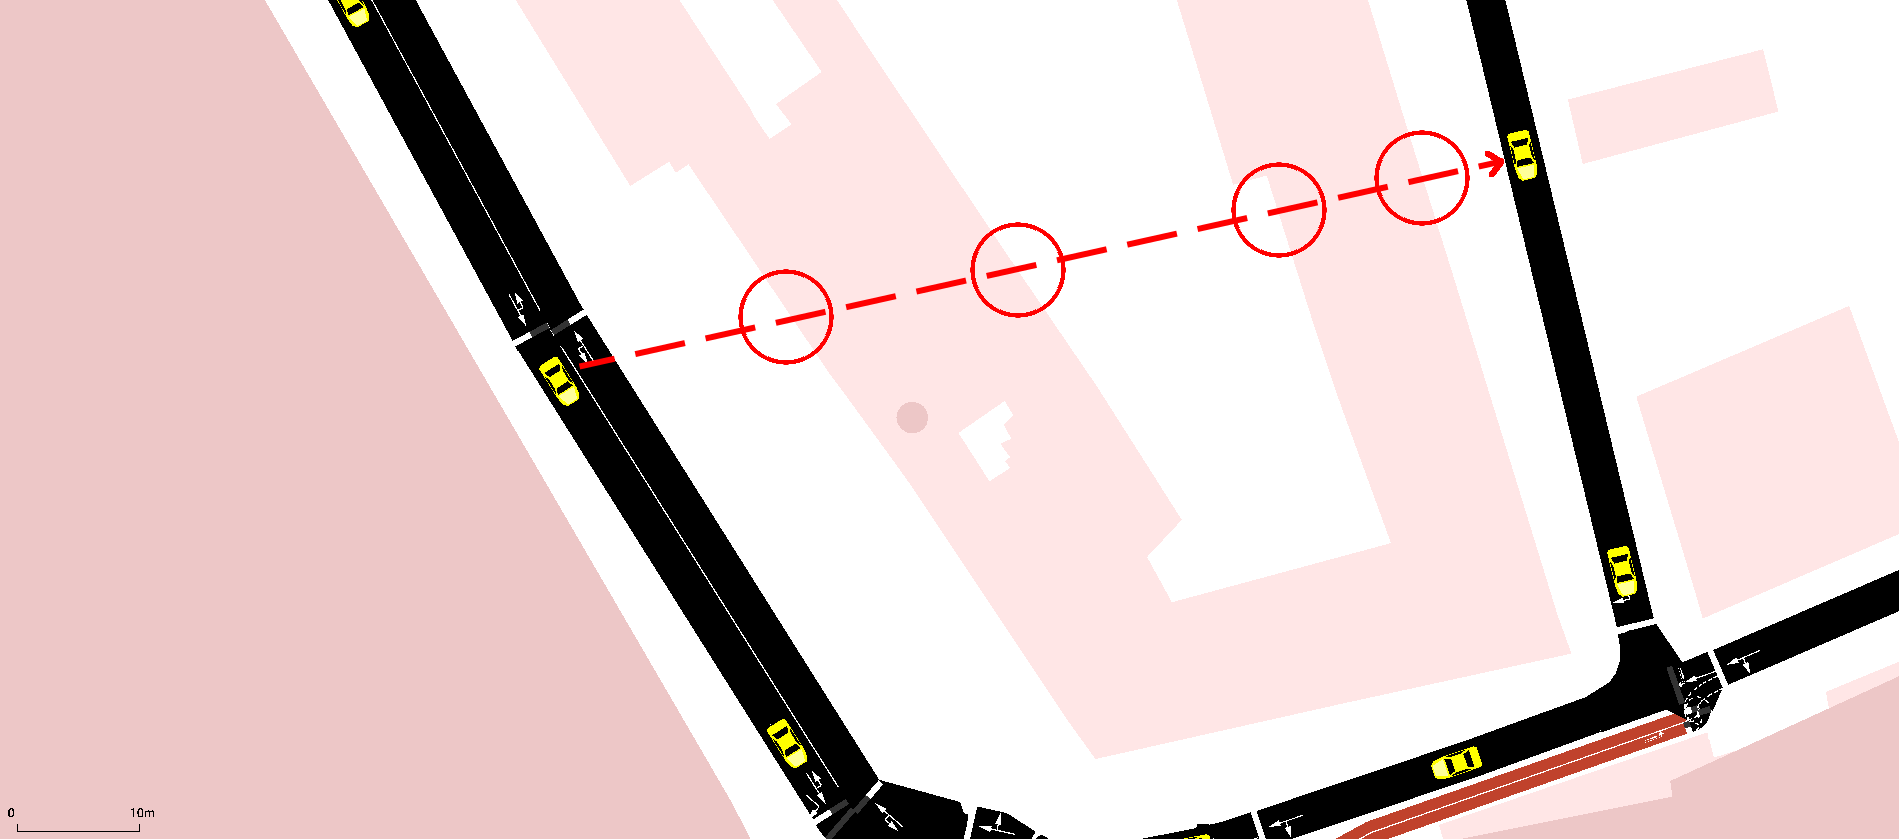
\includegraphics[width=\textwidth]{immagini/sumo-obstacle}
			\caption{Example of obstacle shadowing in vehicle-to-vehicle communication. Walls encountered by the signal are surrounded in red circles}
			\label{fig:sumo-obstacle}
		\end{figure}
	
	\section{Emergency Message Dissemination and broadcasting protocols}
		\label{sec:emd}
		Emergency Message Dissemination (EMD) is a fundamental application in \acrshort{vaneta} to prevent traffic accidents, thereby reducing death and injury rates. Such task can be execute by the VANET itself by turning it into an infrastructure-less self-organizing network, where the dissemination is carried out by specific protocols. 
		
		
		Since the traffic information, especially the emergency data, has a broadcast-oriented nature (i.e. it is of public interest), it is more appropriate to disseminate it using broadcasting routing scheme rather than unicast or multicast ones. \cite{5989903}
%		suddivisione broadcasting protocols
		
		This choice leads to some advantages, such as:
		\begin{itemize}
			\item the fact that vehicles do not need to know the destination address and how to calculate a route towards it;
			\item a greater coverage of vehicles interested in the information, useful also in lossy scenarios, especially when paired with controlled redundancy schemes;
			\item a greater efficiency in bandwidth usage.
		\end{itemize}
		
		The idea behind existing algorithms consists in designating the next forwarder in the multi-hop chain from the source of the alert to the target region where the sensitive data has to be delivered. Ideally, the farthest vehicle from a previous forwarder in the dissemination direction should be given priority when designating the next forwarder. However, due to unreliable wireless channel the designation of farthest vehicle can fail and interrupt the message dissemination. Due to this, next forwarder designation keeps into consideration vehicles (called potential forwarder candidates, PFCs) which have received an Alert Message. The PFCs participate in contention to elect the farthest forwarder candidate (FFC) who will continue disseminating the message.
		
		
		In order to carry out the forwarder designation process, the main idea consists in differentiating waiting times (WT) of PFCs. Each PFC should select a waiting time ranging from 0 to a predefined upper bound (PUB). To guarantee the correct designation of the farthest vehicle as forwarder, PFCs choose their waiting time inversely proportional to the distance between the PFC and the previous forwarder. This way other candidates can detect the transmission from the FFC and suppress their transmission.
		
		Advancements in research on Emergency Message Dissemination has lead to the development of a number of broadcasting protocols. However, as identified by Panichpapiboon et al.\cite{5989903}, most of them belong to one of two main categories:
		\begin{itemize}
			\item Multi-hop Broadcasting Protocols, in which packets are transmitted through the network via flooding by some of the neighbors of the source. It is of utmost importance to reduce the number of redundant transmission in order not to waste bandwidth.
			\item Single-hop Broadcasting Protocols, in which no flooding is employed. Instead, vehicles periodically select and broadcast only a subset of the packets it has received.
		\end{itemize}
		
		
		Multi-hop Broadcasting Protocols can be further subdivided into two categories:
		\begin{enumerate}
			\item Delay based protocols, which assign a different waiting time before rebroadcasting the message to each vehicle. This delay is usually inversely proportional to the distance between the source and the potential sender.
			Some examples are:
			\begin{itemize}
				\renewcommand\labelitemi{--}
				\item \textit{Urban Multi-hop Broadcast (UMB)} \cite{Korkmaz:2004:UMB:1023875.1023887}, designed to solve the broadcast redundancy, hidden node and reliability problems in multi-hop broadcasting using \textit{Request-to-Broadcast (RTB)} and \textit{Clear-To-Broadcast (CTB)} packets; 
				\item \textit{Smart Broadcast (SB)} \cite{4025102} and \textit{Efficient Directional Broadcast (EDB)} \cite{4340158}, which try to reduce the delay introduced by UMB and remove the RTB and CTB packets, respectively;
				\item \textit{Vehicle-density-based Emergency Broadcasting (VDEB)} \cite{5663803}, a slotted broadcasting protocol which keeps vehicle density into consideration when computing waiting time slots;
				\item \textit{Reliable Method for Disseminating Safety Information
				(RMDSI)} \cite{4591259}, which aims to offer better performances when the network becomes fragmented by making a forwarder keep a copy of the packet it has broadcasted until it hears a retransmission (or until the packet lifetime expires). If no retransmission is heard within a certain time limit, the forwarder tries to find the next node which can relay the message using a small control packet;
				\item \textit{Multi-hop Vehicular Broadcast (MHVB)} \cite{4068699}, a protocol that keeps traffic congestion into consideration by   checking whether the number of neighbors of a vehicle is greather than a certain threshold and its speed is less than another threshold. When a node detects congestion, it increases its broadcast interval in order to try to reduce the network load;
				\item \textit{Reliable Broadcasting of Life Safety Messages (RBLSM)} \cite{4458046}, whose main objective is reliability, and a higher priority is given to the vehicle nearest to the sender instead to the one furthest from it, due to the assumption that the closer the vehicle is, the more reliable it is considered since its received signal strength is higher.
			\end{itemize}
		
			\item Probabilistic-based Multi-hop Broadcasting Protocols
			The idea behind these kind of protocols is similar to the one behind Delay based protocols, but instead of assigning a different rebroadcast delay to each vehicle, a different rebroadcast probability is assigned. Each protocol differs in the function that assigns probabilities. Some examples of probabilistic-based protocols are:
			\begin{itemize}
				\renewcommand\labelitemi{--}
		 		\item \textit{Weighted p-Persistence} \cite{4407231}, in which every PFC computes its own rebroadcast probability based on distance between itself and the transmitter. The formula used is the following:
				\begin{gather}
		 			p_{ij} = \frac{D_{ij}}{R}
		 			\label{eq:weighted-p-persistence}
 				\end{gather}
 				where $D_{ij}$ is the distance between transmitter \textit{i} and PFC \textit{j} and R is the transmission range. Given this function, the probability to rebroadcast is proportional to the distance between the PFC and the transmitter. The abovementioned formula does not keep into account vehicle density and also assumes that the transmission range is fixed and known to all vehicles.
 				
 				\item \textit{Optimized Adaptive Probabilistic Broadcast (OAPB)\cite{1543865} and AutoCast (AC) \cite{4350058}}, which both keep the vehicle density into consideration when computing the forwarding probability by making vehicle periodically exchange Hello messages. Thanks to those messages, each vehicle can compute the number of neighbors and then use this information accordingly.
 				
 				\item \textit{Irresponsible Forwarding (IF)} \cite{4740277}\cite{5426212}, a protocol that considers vehicle density like OAPB and AC, but the formula used is not a simple linear function. In fact, the rebroadcast probability assignment function is the following:
 				\begin{gather}
 					p = e^{-\frac{\rho_s(z-d)}{c}}
 				\end{gather}
 				where $\rho_s$ is the vehicle density, $z$ is the transmission range, $d$ is the distance between the PFC and the transmitter and $c\geq1$ is a shaping parameter which influences rebroadcast probability. Irresponsible Forwarding aims to offer a solution that can scale with network density.
			\end{itemize}
		
%		\item Network Coding-Based Multi-hop Broadcasting. TODO? da fare?
		
		Vehicles employing Single-Hop Broadcasting protocols will not flood received packets immediately through the network. Instead, vehicles use information from packets to update their database and periodically rebroadcast only a fraction of that information. The two variables these kind of protocol can work on to aim for good network efficiency are:
		\begin{itemize}
			\item \textit{Broadcast Interval}, i.e. the amount of time between retransmissions, which should keep into consideration both freshness of information and potential redundancy in transmissions;
			\item \textit{Relevancy of information} to broadcast: as stated before, only relevant information (i.e. a subset of all the information) should be broadcast.
		\end{itemize}
		
		Single-Hop protocols can be further subdivided into two categories:
		\begin{enumerate}
			
			\item Fixed Broadcast Interval, which keep the Broadcast Interval fixed. Some exampels are:
			\begin{itemize}
				\renewcommand\labelitemi{--}
				
				\item \textit{TrafficInfo}\cite{4621303}, a protocol in which vehicles record, among other information, travel times on road segments (identified by an ID) and keep them on its on-board database. Vehicles periodically exchange information about the learned travel times based on the relevance of such information. The relevance is calculated using a ranking algorithm which uses the current position of the vehicle and the current time (i.e. relevance decreases with distance and time), broadcasting only the $k$  most important information. 
				
				\item \textit{TrafficView}\cite{1263039}, in which vehicles exchange information about speed and position and record it in their database. Data about different vehicles is then aggregated into a single record using one of two aggregation algorithms:
				\begin{itemize}
					\item the \textit{ratio-based} algorithm, which assigns an aggregation ratio to each portion of a road: the more important the road is, the higher the aggregation ratio will be, increasing the accuracy of the information of that area.
					\item the \textit{cost-based} algorithm, an algorithm which keeps into consideration the cost of aggregating different records. The aggregation cost is defined as the loss of accuracy the aggregation will bring about.
				\end{itemize} 
			\end{itemize}
			\item Adaptive Broadcast Interval, which adapt the Broadcast Interval based on dynamic information. Some examples are:
			\begin{itemize}
				\renewcommand\labelitemi{--}
				
				\item \textit{Collision Ratio Control Protocol (CRCP)}\cite{4357748}, a scheme according to which vehicles exchange information about location, speed and road ID. The Broadcast Interval is dynamically controlled based on the amount of detected collisions and bandwidth efficiency: the protocol tries to maintain the number of collisions under a certain threshold by doubling the Broadcast Interval every time the threshold is exceeded. Otherwise, the Broadcast Interval is decreased by one second when the bandwidth efficiency decreases too much.
				
				Moreover, the authors propose three different methods for selecting the data to be transmitted:
				\begin{itemize}
					\item \textit{Random Selection}: a vehicle selects a random information in its database and broadcasts it;
					\item \textit{Vicinity Priority Selection}: vehicles give priority to information of nearby areas;
					\item \textit{Vicinity Priority Selection with Queries}: similar to Vicinity Priority Selection, with the possibility of querying information for a certain area.
				\end{itemize}
				
				\item \textit{Abiding Geocast:}\cite{4531929}, which aims to deliver an Alert Message to a specific area where the warning is still relevant. Only vehicles that are travelling towards the effective area can participate in contention to broadcast the message. Moreover, broadcast is dynamically adjusted based on transmission range, speed, and distance between the potential forwarder and the destination area, increasing when such distance increases or the potential forwarder's speed decreases.
				
				\item \textit{Segment-oriented Data Abstraction and Dissemination
					(SODAD)}\cite{1402433}, a protocol according to which roads are divided into segments and each vehicle can both discover information itself and collect it from neighbor's transmissions. Whenever a vehicle receives a transmission from another vehicle, the information received will be classified as either one of two events:
					\begin{itemize}
						\item a \textit{provocation} event that will decrease the Broadcast Interval;
						\item a \textit{mollification} event that will increase the Broadcast Interval.
					\end{itemize}
					The classification is done via comparison of the newly received data with the information stored in the vehicle's on-board database. The vehicle assigns a higher weight if the difference between information coming from these two sources is high. The weight will be then compared against a threshold to establish whether a provocation of mollification event has taken place.
			\end{itemize}
		
		The authors of ROFF \cite{6906275}, a Multi-Hop delay based protocol, state that existing protocols are affected by two problems:
		\begin{itemize}
			\item the perfect suppression of redundant transmissions, by which potential forwarders which have lost the contention detect the transmission from the farthest vehicle and suppress their transmission. However this suppression can not always be guaranteed due to short difference between waiting times. In fact, if the timer of a potential forwarder expires before it has heard the transmission from the FFC, a redundant transmission will occur;
			\item the disuniformity and the costant change in spatial vehicle distribution in VANETs. Existing protocols which keep into consideration the distance between PFC and previous forwarder do not keep into consideration large empty spaces in the waiting time computation, leading to unnecessary wait.
		\end{itemize}
		ROFF's solutions to these problems and the implementation of the protocol will be analyzed in Chapter \ref{chapter:roff}
		
%		The previous thesis \cite{ROM2017} focused on the evaluation of Fast Broadcast \cite{4199282}, a Multi-Hop delay based protocol, through simulation in various scenarios. 
			
		\end{enumerate}
		
		\end{enumerate}  
% !TEX encoding = UTF-8
% !TEX TS-program = pdflatex
% !TEX root = ../tesi.tex

\chapter{Fast Broadcast}
	Fast Broadcast \cite{4199282} is a multi-hop routing protocol for vehicular communication. Its main feature consists in breaking the assumption that all vehicles should know, a priori, their fixed and constant transmission range. This assumption is often unreasonable, especially in \acrshort{vaneta}s and urban environments, where electromagnetic interferences and obstacles such as buildings heavily influence the transmission range.
	
	
	Fast Broadcast employs two different phases:
	\begin{enumerate}
		\item the \textbf{Estimation Phase}, during which cars estimate their frontward and backward transmission range;
		\item the \textbf{Broadcasts Phase}, during which a car sends an Alert Message and the other cars need to forward it in order to propagate the information.
	\end{enumerate}

	\section{Estimation Phase}
		During this phase, cars try to estimate their frontward and backward transmission range by the means of Hello Messages. These beacons are sent periodically via broadcast to all the neighbors of a vehicle.
		
		
		Time is divided into turns and, in order to keep estimations fresh, data collected during a certain turn is kept for the duration of the next turn, then discarded. The parameter \textit{turnSize} specifies the duration of a turn: the authors suggest a duration of one second. A bigger \textit{turnSize} could guarantee less collisions to the detriment of freshness of information. On the other hand, the effects of a smaller \textit{turnSize} are specular to those just presented. 
		
		
		Using this approach, vehicles can estimate two different values:
		\begin{itemize}
			\item \textit{Current-turn Maximum Front Range (CMFR)}, which estimates the maximum frontward distance from which another car can be heard by the considered one;
			\item \textit{Current-turn Maximum Back Range} (CMBR), which estimates the maximum backward distance at which the considered car can be heard.
		\end{itemize}
		When the turn expires, the value of these variables is stored in the LMFR and LMBR variables (\textit{Latest-turn Maximum Front Range} and \textit{Latest-turn Maximum Back Range}, respectively). The algorithm uses both last turn and current turn data because the former guarantees values calculated with a larger pool of Hello Messages, while the latter considers fresher information.
		
		When sending a Hello Message (Algorithm \ref{alg:hello-message-sending}), the vehicle initially waits for a random time between 0 and \textit{turnSize}. After this, if it has not heard another Hello Message or a collision, it proceeds to transmit a Hello Message containing the estimation of its frontward transmission range.
		
		
		When receiving a Hello Message (Algorithm \ref{alg:hello-message-receiving}), the vehicle retrieves its position and the sender's position, calculates the distance between these two positions and then updates the CMFR field if the message comes from ahead, otherwise CMBR is updated. The new value is obtained as the maximum between the old CMFR or CMBR value, the distance between the vehicle and the sender, and the sender's transmission range estimation included in the Hello Message.
		
		\begin{algorithm}[H]
			\begin{algorithmic}[1]
				\ForEach{turn}
					\State sendingTime $\gets$ random(turnSize)
					\State wait(sendingTime)
					\If{$\neg$ (heardHelloMsg() $\lor$ heardCollision())}
						\State helloMsg.declaredMaxRange $\gets$ max(LMFR, CMFR)
						\State transmit(helloMsg)
					\EndIf
				\EndFor
			\end{algorithmic}
			\caption{Hello message sending procedure}
			\label{alg:hello-message-sending}
		\end{algorithm}
		
		\begin{algorithm}[H]
			\begin{algorithmic}[1]
				\State mp $\gets$ myPosition()
				\State sp $\gets$ helloMsg.senderPosition
				\State drm $\gets$ helloMsg.declaredMaxRange
				\State d $\gets$ distance(mp, sp)
				\If{receivedFromFront(helloMsg)} 
				\State CMFR $\gets$ max(CMFR, d, drm)
				\Else
				\State CMBR $\gets$ max(CMBR, d, drm)
				\EndIf
			\end{algorithmic}
			\caption{Hello message receiving procedure}
			\label{alg:hello-message-receiving}
		\end{algorithm}
	
	\section{Broadcast Phase}
		This phase is activated once a car sends an Alert Message. The other cars can exploit the estimation of transmission ranges to reduce redundancy in message broadcast. Each vehicle can exploit this information to assign itself a forwarding priority inversely proportional to the relative distance: the higher the relative distance, the higher the priority.  
		
		
		When the Broadcast Phase is activated , a vehicle sends an Alert Message with application specific data. Broadcast specific data is also piggybacked on the Alert Message, such as:
		\begin{itemize}
			\item \textit{MaxRange:} the maximum range a transmission is expected to travel backward before the signal becomes too weak to be received. This value is utilized by following vehicles to rank their forwarding priority;
			\item \textit{SenderPosition}: the coordinates of the sender.
		\end{itemize}
		Upon reception, each vehicle waits for a random time called \textit{Contention Window} (\textit{CW}). This window ranges from a minimum value (\textit{CWMin}) and a maximum one (\textit{CWMax}) depending on sending/forwarding car distance (\textit{Distance}) and on the estimated transmission range (\textit{MaxRange}), according to formula \ref{eq:contention-window}. It is quite easy to see that the higher the sender/forwarder distance is, the lower the contention window is.
		\begin{gather}
			\left\lfloor \left( \frac{\text{MaxRange} - \text{Distance}}{\text{MaxRange}} \times (\text{CWMax} - \text{CWMin}) \right) + \text{CWmin}  \right\rfloor
			\label{eq:contention-window}
		\end{gather}
		If another forwarding of the same message coming from behind is heard during waiting time, the vehicle suppresses its transmission because the message has already been forwarded by another vehicle further back in the column. On the contrary, if the same message is heard coming from the front, the procedure is restarted using the new parameters. The vehicle can forward the message only if the waiting time expires without having received the same message.
		
		Algorithm \ref{alg:alert-message-generation} and \ref{alg:alert-message-forwarding} describe the logic behind the Broadcast Phase.
		
		\begin{algorithm}[H]
			\begin{algorithmic}[1]
				\State alertMessage.maxRange $\gets$ max(LMBR, CMBR)
				\State alertMessage.position $\gets$ retrievePosition()
				\State transmit(alertMessage) $\gets$ helloMsg.declaredMaxRange
			\end{algorithmic}
			\caption{Alert Message generation procedure}
			\label{alg:alert-message-generation}
		\end{algorithm}
	
		\begin{algorithm}[H]
			\begin{algorithmic}[1]
				\State cwnd $\gets$ computeCwnd()
				\State waitTime $\gets$ retrievePosition()
				\State wait(waitTime
				\If{sameBroadcastHeardFromBack()}
				\State exit()
				\ElsIf{sameBroadcastHeardFromFront()}
				\State restartBroadcastProcedure()
				\Else 
				\State maxRange $\gets$ max(LMBR, CMBR)
				\EndIf 
			\end{algorithmic}
			\caption{Alert Message generation procedure}
			\label{alg:alert-message-forwarding}
		\end{algorithm}
	
	\section{Two dimensions extension}
		The original work \cite{4199282} considered only a strip-shaped road, where it was easy to define directions and establish 	when a message came from the front or the back. In \cite{BAR2017} an extension considering two dimensions was proposed. 
		
		
		The modifications to the Fast Broadcast algorithm are the following:
		\begin{enumerate}
			\item Utilizing only one parameter between CMBR and CMFR (thus considering only CMR):
			\item Including the position of the vehicle which originally generated the Alert Message in addition to the position of the sender of the message.
		\end{enumerate}
		
		
		When a vehicle receives an Alert Message, the origin-vehicle distance is confronted with the origin-sender distance: the vehicle can forward the message only if the former is greater than or equal to the latter, otherwise it simply discards the message.
		
		\begin{figure}[H]
			\centering
			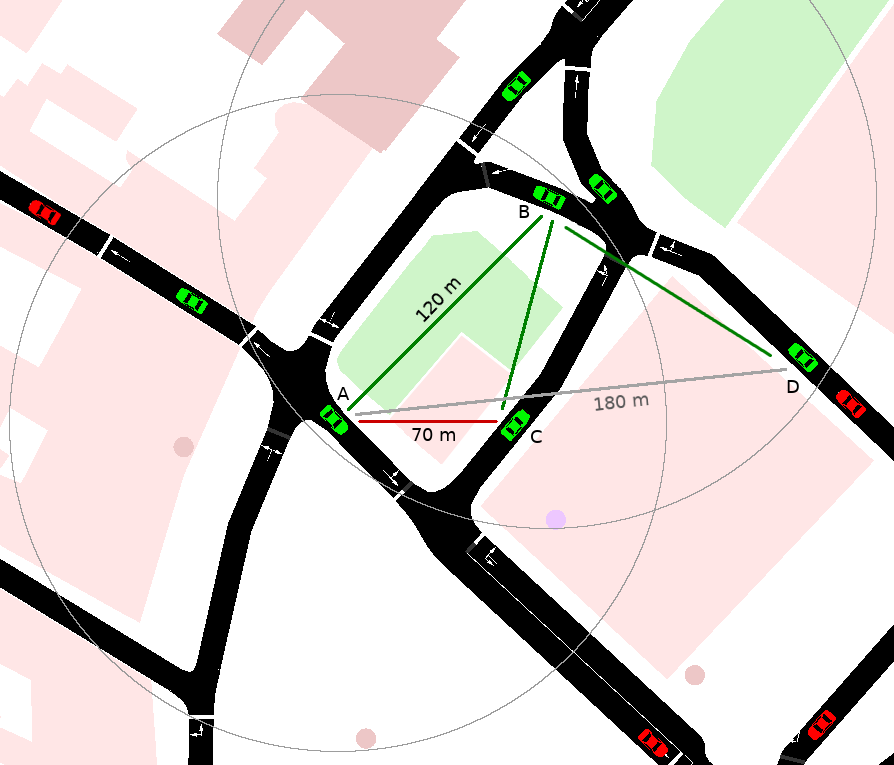
\includegraphics[width=\textwidth]{immagini/fb-2dpicc}
			\caption{Example of Fast Broadcast in 2d scenario}
			\label{fig:fb-2d}
		\end{figure}
		
		
		
		For example, suppose that vehicle A is the origin of the Alert Message and B receives it, but C doesn't due to an obstacle in the line of sight. B computes origin-vehicle distance, $d(A, B)$, and origin-sender distance, $d(A, A)$, which in this case are respectively 120 and 0m. Since origin-vehicle is greater than origin-sender, B can forward the Alert Message.
		
		
		Now suppose that C receives the message from B. C computes origin-vehicle distance, $d(A, C)$, and origin-sender distance, $d(A, B)$, which amount to 70 and 120m respectively. Since the former is not greater than or equal to the latter, C is not a candidate for forwarding and suppresses the transmission.
		
		
		D receives the message from B as well. D is a good candidate for transmission since the origin-vehicle distance, which amounts to 180m, is greater than origin-sender distance, equal to 120m.

%\chapter{L'offerta di \textit{stage}}
%\label{cap:loffertadistage}
%
%\section{\textit{Stage} in IBC: motivazioni aziendali}
%	\label{sec:motivazioni_aziendali}
%	IBC è un'azienda che in passato ha già offerto rapporti di \textit{stage}, anche se questo è il primo anno che essa partecipa a StageIt. Per non essere una perdita di tempo e risorse aziendali, gli \textit{stage} in IBC devono avere obiettivi e motivazioni che portano vantaggi anche a quest'ultima, oltre che allo stagista.
%	
%	\begin{itemize}
%		\item Il primo obiettivo che l'azienda tenta di raggiungere è lo studio di nuove tecnologie per andare ad espandere (e in alcuni casi sostituire) gli strumenti utilizzati. I dipendenti di IBC infatti sono quasi sempre impegnati in progetti con scadenze stringenti, il che rende molto difficile dedicare risorse alla scoperta e all'apprendimento di nuove tecnologie. Questi compiti sarebbero solitamente svolti dal reparto ricerca e sviluppo, assente in IBC. Le attività svolte durante lo \textit{stage} coprono quindi in parte questa mancanza, permettendo all'azienda di ottenere informazioni su nuovi strumenti e \gls{proofofconcept} di prodotti di futura realizzazione.
%		
%		
%		\item Il secondo obiettivo riguarda la prospettiva di assunzione di nuovo personale. L'azienda infatti tratta lo \textit{stage} come periodo di prova pre-assunzione, in modo da poter verificare le capacità dello stagista e fargli apprendere i meccanismi aziendali. IBC, al momento dell'offerta, era alla ricerca di programmatori Java e ha presentato una proposta proprio in quell'ambito. Assumere il tirocinante nello stesso ambito alla fine dello \textit{stage} fa risparmiare all'azienda tempo e risorse rispetto a un ulteriore addestramento in un'altra area.
%		
%		
%		\item La terza e ultima motivazione è il vantaggio che IBC può ottenere da una mente giovane e creativa, come ad esempio quella di uno studente che sta per concludere una laurea triennale in Informatica. Al contrario del personale abituato da anni a portare a termine gli stessi compiti nella stessa maniera, uno studente è più propenso ad inventare soluzioni originali e talvolta non convenzionali. Non sempre è detto che tali soluzioni siano adottabili e manutenibili, quindi è necessaria una revisione da parte di personale esperto prima che l'azienda adotti le proposte dello stagista.
%	\end{itemize}
%
%\section{Il progetto}
%
%	\subsection{Dominio applicativo}
%		Il progetto di \textit{stage} riguardava la memorizzazione di informazioni di prodotti commerciali. Il continuo rapporto con clienti in ambito \gls{retail} da parte di IBC porta alla necessità di avere una persistenza delle informazioni dei prodotti che essi offrono sul mercato. 
%		
%		\begin{figure}[H]
%			\centering
%			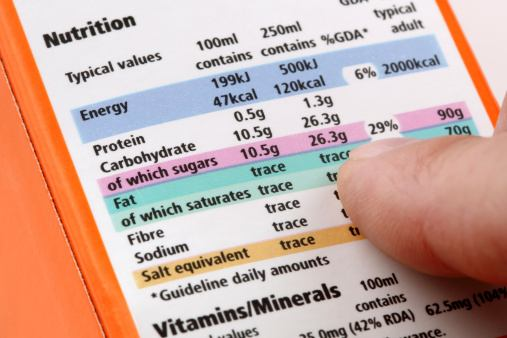
\includegraphics[scale=0.5]{immagini/etichetta}
%			\caption{Informazioni di un prodotto (\url{goo.gl/pxeYU1}).}
%		\end{figure}
%		
%		Questi dati sono utilizzati in molti ambiti, come ad esempio:
%		\begin{itemize}
%			\item La stampa dell'etichetta da apporre sulla confezione di un prodotto.
%			\item La categorizzazione di tipologie di prodotto sugli scaffali di un supermercato o sul sito di un \textit{e-commerce}.
%			\item L'identificazione e la ricerca di prodotti con particolari caratteristiche.
%			\item La gestione di magazzino.
%			\item L'identificazione di allergeni o particolari agenti chimici.
%			\item La raccolta di dati statistici e la generazione di reportistica.
%		\end{itemize}
%		
%		Dati i molti utilizzi, la memorizzazione delle informazioni è una necessità che negli anni ha avuto varie soluzioni e implementazioni.
%						
%		Attualmente IBC utilizza un \textit{database} relazionale per la persistenza dei dati. Questo porta al problema principale che il progetto offerto deve risolvere. Data la natura stessa del modello relazionale, è necessario definire una struttura prima di poter memorizzare un qualsiasi elemento. Gli attributi dei prodotti però sono variabili e non è raro trovare due prodotti appartenenti alla stessa categoria con qualche attributo non in comune.
%		
%		Un altro fattore da considerare è il fattore umano: dato che le informazioni dei prodotti vengono spesso fornite a IBC da personale non tecnico, capita a volte che gli attributi non rispettino i limiti imposti dalla struttura relazionale, portando all'impiego di risorse per riprogettare la struttura o tradurre gli attributi in un modello valido.
%		
%		Tenendo conto dei due punti appena esposti, l'attuale soluzione adottata dall'azienda prevede la definizione di una struttura che contempli tutti i possibili attributi di ogni categoria di prodotto. Le particolari istanze di ogni prodotto che non riportano un qualche attributo avranno il valore di quest'ultimo impostato a \texttt{null}.
%		
%		Questa soluzione è però poco logica ed è imposta dal modello relazionale. Un \textit{Content Repository} fornisce un'alternativa senza lo svantaggio appena esposto.
%		
%		IBC era quindi alla ricerca di una soluzione flessibile, che permettesse l'aggiunta di prodotti aventi proprietà variabili, utilizzando il modello JCR. Il \textit{tutor} ha affermato che l'obiettivo del prototipo da realizzare era verificare se fosse possibile implementare una soluzione utilizzando la libreria \gls{jackrabbit}. Anche in base ai risultati da me ottenuti, l'azienda deciderà in futuro se intraprendere un progetto su più ampia scala per la realizzazione di un \textit{software} utilizzando questa tecnologia.
%		
%		
%		\subsection{Introduzione a JCR}
%		Date le mie scarse conoscenze del dominio del progetto, ho impiegato i primi giorni lavorativi per effettuare uno studio preliminare. Ho consultato principalmente risorse presenti \textit{online}, tra cui:
%		\begin{itemize}
%			\item \textit{Paper} \jquote{JCR or RDBMS: why, when, how?}, per comprendere le differenze tra Relational DataBase Management System (d'ora in poi RDBMS) e Java Content Repository (d'ora in poi JCR).
%			\item Articolo \jquote{What is Java Content Repository} (\url{https://goo.gl/8HWDRZ}), per avere una descrizione di base di JCR.
%			\item Standard \gls{jsr170} e \gls{jsr283}.
%		\end{itemize}
%		
%		I risultati delle mie ricerche sono contenuti all'interno di due documenti che ho prodotto per IBC:
%		\begin{itemize}
%			\item \textbf{Confronto tra RDBMS e JCR:} documento che racconta la storia di JCR e analizza le differenze tra il modello relazionale e il modello JCR.
%			\item \textbf{Struttura JCR e funzionamento Jackrabbit:} documento che, a partire dagli \textit{standard} precedentemente citati, fornisce una spiegazione delle principali API per l'accesso a JCR. Inoltre, date le funzionalità aggiuntive fornite da Jackrabbit, nella seconda parte del documento descrivo la struttura di Jackrabbit e il suo funzionamento nel dettaglio.
%		\end{itemize}
%		
%		Un \textit{Content Repository} è un modello utilizzato per la memorizzazione di qualsiasi tipo di dato. Gli \textit{standard} \gls{jsr170} e \gls{jsr283} definiscono le API per JCR.
%		
%		Le differenze tra il modello relazionale e il JCR possono essere suddivise in varie aree, come analizzato nel seguente \textit{paper}:
%		\url{https://goo.gl/ngzgKt}.
%		
%		\begin{figure}[H]
%			\centering
%			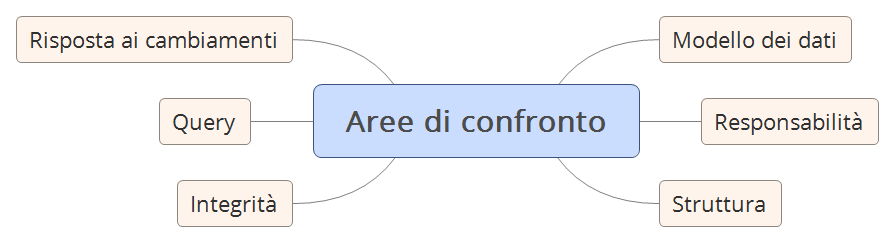
\includegraphics[scale=0.4]{immagini/aree-confronto}
%			\caption{Aree di confronto tra RDBMS e JCR.}
%		\end{figure}
%		
%		\begin{enumerate}
%			\item \textbf{Modello dei dati} \\
%			Con \jquote{modello dei dati} intendiamo il modo con cui i dati vengono organizzati, acceduti e messi in relazione tra di loro.
%			\paragraph{RDBMS} 
%			Il modello relazionale si basa sulla teoria degli insiemi e sulla definizione matematica di relazione, che ricordiamo essere un sottoinsieme del prodotto cartesiano tra \textit{n} insiemi. Dato che ognuno di questi dev'essere distinguibile dagli altri, ogni insieme è definito come dominio. Ad esempio, facendo riferimento alla tabella sottostante, i domini sono quello dei nomi (N), cognomi (C) ed età (E). 
%			
%			\begin{figure}[H]
%				\centering
%				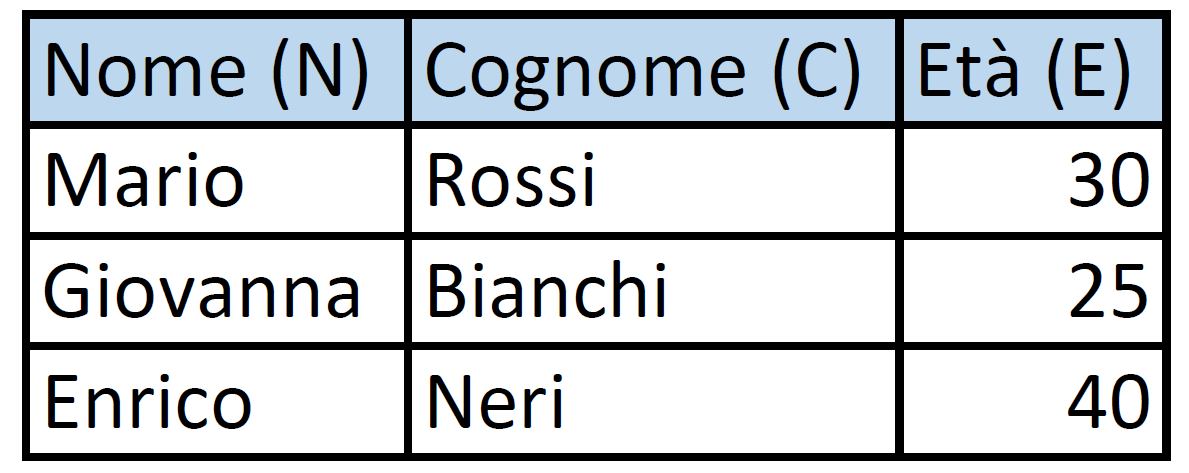
\includegraphics[scale=0.2]{immagini/modello-r}
%				\caption{Tabella che rappresenta una persona (\url{https://goo.gl/ngzgKt}).}
%			\end{figure}
%		
%			La definizione di relazione non implica la possibilità di creare associazioni tra le relazioni. Per fare questo, è necessario utilizzare l'algebra relazionale. 
%			
%			\paragraph{JCR} 
%			Il modello JCR si basa principalmente su una struttura ad albero, unendo le caratteristiche dei modelli gerarchici a quelle dei modelli a rete. Il risultato è una struttura ad albero che permette la connessione dei nodi orizzontalmente.
%			
%					\begin{figure}[H]
%						\centering
%						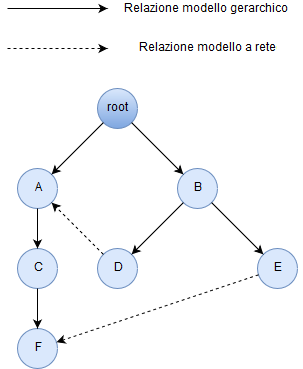
\includegraphics[scale=0.5]{immagini/modello-j}
%						\caption{Unione del modello a rete con il modello gerarchico (\url{https://goo.gl/ngzgKt}).}
%					\end{figure}
%				
%			\item \textbf{Responsabilità} \\
%			Quando si tratta di \textit{database} e persistenza dei dati, generalmente possono essere identificati tre ruoli principali:
%			\begin{itemize}
%				\item Il \textbf{\textit{database administrator} (DBA)}, che mantiene il \textit{database} in uno stato utilizzabile eseguendo attività di installazione, configurazione, \textit{backup} e \textit{data recovery}.
%				\item L'\textbf{\textit{application programmer}}, che scrive \textit{software} che accede al \textit{database}.
%				\item L'\textbf{utente}, che utilizza il \textit{software} per leggere, scrivere e modificare i dati nel \textit{database}.
%			\end{itemize}
%			I due modelli si differenziano anche sotto il punto di vista dei ruoli. Più precisamente, cambiano le responsabilità e i campi di interesse di ogni ruolo.
%			
%			
%			I campi di interesse presi in esame sono:
%			\begin{itemize}
%				\item \textbf{Contenuto}: tutti i dati inclusi nel \textit{database}.
%				\item \textbf{Struttura}: il modo con cui i dati sono suddivisi.
%				\item \textbf{Integrità}: lo stato di completezza dei dati.
%				\item \textbf{Coerenza}: la relazione ordinata, logica e consistente delle parti.
%			\end{itemize}
%			
%			
%			\paragraph{RDBMS} 
%				Nel modello relazionale generalmente è il DBA ad avere il controllo sulla struttura. L'\textit{application programmer} solitamente ha un qualche tipo di influenza sulle decisioni prese in questo campo, ma la decisione finale spetta al DBA. L'utente non ha alcuna responsabilità per quanto riguarda la struttura e può solo interagire con il \textit{database} tramite le operazioni fornite dal \textit{software}.
%				
%				\begin{figure}[H]
%					\centering
%					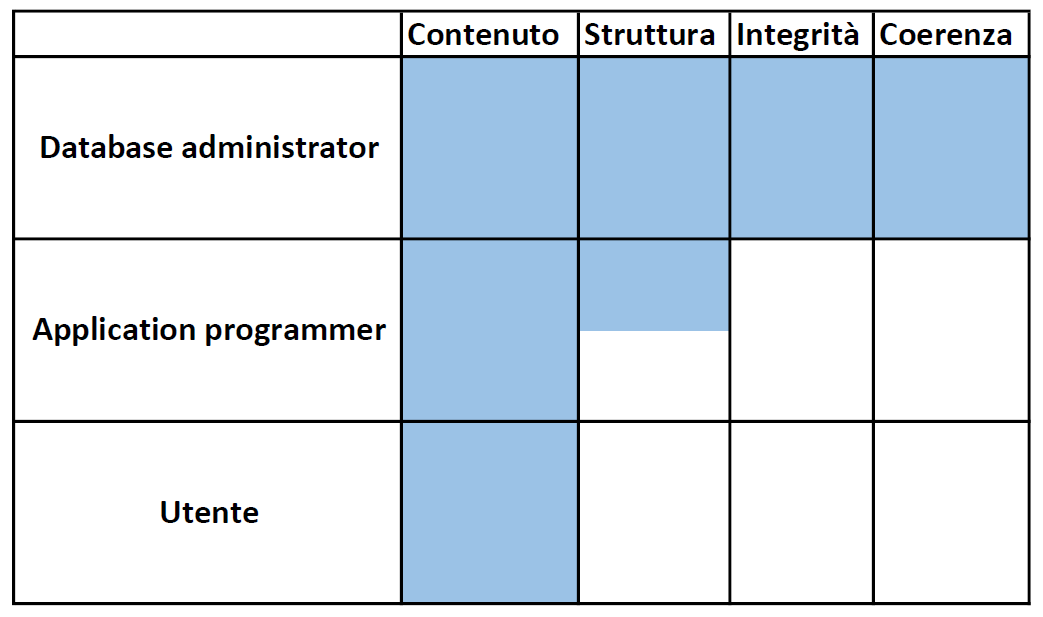
\includegraphics[scale=0.4]{immagini/ruoli-r}
%					\caption{Responsabilità dei ruoli in RDBMS (\url{https://goo.gl/ngzgKt}).}
%				\end{figure}
%			
%			
%			\paragraph{JCR} 
%				Nel modello JCR invece la struttura è responsabilità di tutti e tre i ruoli. Infatti, il controllo sulla struttura è più incentrato verso l'\textit{application programmer} e l'utente, riducendo di fatto le responsabilità del DBA in questo campo.
%				
%				
%				Uno dei vantaggi principali di questo approccio è che solitamente il ruolo di \textit{application programmer} è più vicino all'utente finale rispetto al DBA, quindi una collaborazione tra questi due ruoli per la definizione della struttura è solitamente più efficace.
%				
%				
%				È anche possibile costruire \textit{software} che permettono al solo utente finale di definire la struttura, aggiungendo attributi ai dati a tempo di esecuzione, sottostando ai vincoli definiti dal DBA e dall'\textit{application programmer}.
%				
%				\begin{figure}[H]
%					\centering
%					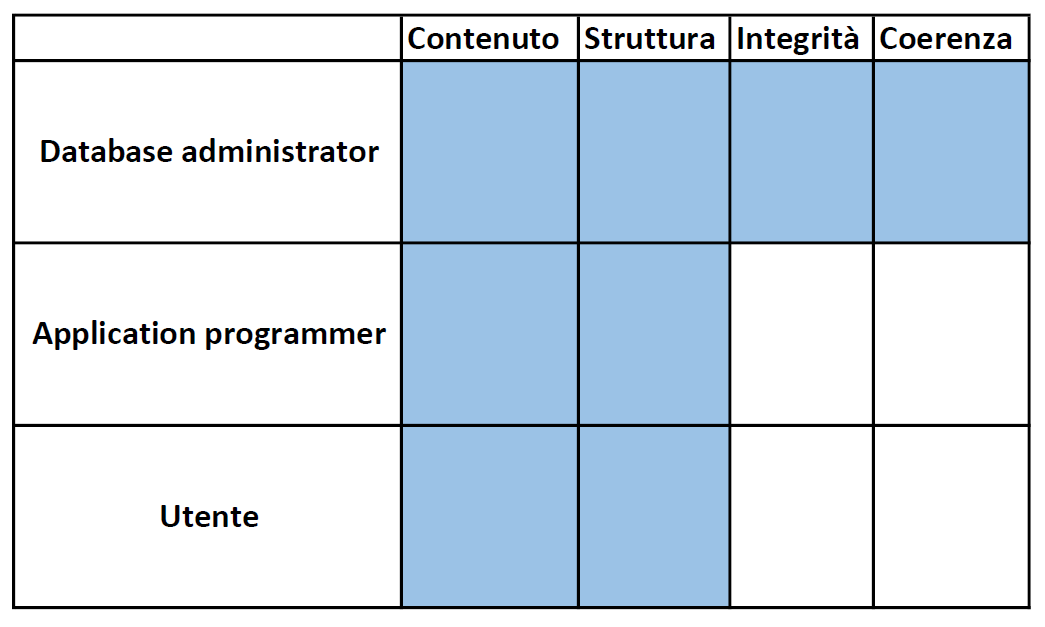
\includegraphics[scale=0.4]{immagini/ruoli-j}
%					\caption{Responsabilità dei ruoli in JCR (\url{https://goo.gl/ngzgKt}).}
%				\end{figure}
%				
%				\item \textbf{Struttura} \\
%					Con \jquote{struttura} intendiamo il modo con cui i dati sono suddivisi e a quali costrizioni essi sono sottoposti. 
%					
%					
%					Le differenze in termini di struttura rendono i due modelli diametralmente opposti, con vantaggi e svantaggi in entrambi gli approcci.
%					
%					\paragraph{RDBMS} 
%						Nel modello RDBMS, i dati sono guidati dalla struttura. Un dato, per essere istanziato, ha bisogno che la struttura sia completamente definita. Questo modello si basa sull'assunzione che dati e struttura siano sempre completamente separati e indipendenti, ma nella realtà quest'assunzione non è sempre valida. Come esposto precedentemente, ci sono casi d'uso in cui la struttura del dato cambia nel tempo, portando all'aggiunta di nuovi campi o ad un'intera riprogettazione nei casi più sfortunati.
%					
%					\paragraph{JCR} 
%						In JCR non è richiesta la definizione di alcuna struttura per istanziare i dati. Nodi, attributi e valori possono essere creati senza nessun prerequisito. Infatti, la struttura emerge con l'inserimento dei dati. Con il modello JCR non è più necessario definire tutti i possibili attributi al momento della creazione di un tipo di dato, garantendo una maggiore flessibilità ed estendibilità.
%						
%				
%				
%				\item \textbf{Integrità} \\
%					L'integrità di un \textit{database} indica l'impossibilità di distruzioni e alterazioni dei dati, siano esse accidentali o intenzionali. Questa caratteristica è implementata in diversi modi a seconda del modello.
%					
%					\paragraph{RDBMS} 
%						Il modello relazionale adotta una strategia simile ad una \textit{white list}, ovvero i dati possono essere salvati solo se è definita una struttura. È quindi quest'ultima che garantisce buona parte dell'integrità, ad esempio attraverso i vincoli di dominio.
%					
%					
%					\paragraph{JCR} 
%						In opposizione al modello RDBMS, JCR si basa su un approccio a \textit{black list}. Un nodo generico del \textit{Content Repository} può avere qualunque nodo figlio e qualsiasi proprietà, senza vincoli su tipi e valori.
%						
%						
%						Eventuali vincoli possono essere imposti assegnando ai nodi dei tipi. Un tipo di nodo descrive vincoli sul tipo dei nodi figli o sui valori delle proprietà che il nodo stesso può avere. Assegnando un tipo anche ai nodi figli e continuando a procedere in questo modo è possibile imporre sempre più limiti alla struttura.
%						
%				\item \textbf{\textit{Query}} \\
%					Anche il tipo e la potenza delle \textit{query} differenzia i due modelli.
%				
%					\paragraph{RDBMS} 
%						Data la definizione di relazione, il modello RDBMS si basa sull'algebra relazionale per la definizioni delle operazioni di base. Il vantaggio di questo modello è che sia l'\textit{input} che l'\textit{output} delle operazioni sono relazioni. È quindi possibile concatenare espressioni complesse senza troppe difficoltà. Inoltre, la maggior parte dei linguaggi di \textit{query} fornisce anche la possibilità di effettuare cambiamenti sequenziali al risultato di una \textit{query}.
%					
%					
%					\paragraph{JCR} 
%						Nel JCR è necessario utilizzare un modello di \textit{query} astratto per effettuare operazioni. Questo modello astratto serve a mappare il modello JCR con le nozioni di relazione, domini, tuple e attributi tipiche del modello relazionale.
%						
%						
%						Uno dei principali svantaggi è che, con l'implementazione JCR di \textit{default}, non è possibile effettuare cambiamenti sequenziali con una \textit{query}.
%					
%					
%						Nel complesso, JCR offre un supporto più limitato rispetto al modello relazionale per quanto riguarda le \textit{query}, ma ha vantaggi prestazionali nell'esecuzione di ricerche \gls{fulltext}.
%					
%				\item \textbf{Risposta ai cambiamenti} \\
%					Nonostante un'analisi dei requisiti svolta in maniera impeccabile, è possibile che nuovi requisiti emergano dopo che l'architettura di un sistema è già stata definita. Un modello di sviluppo non strettamente sequenziale, come ad esempio quello incrementale, permette solitamente di soddisfare i nuovi requisiti senza dover riprogettare interamente il sistema. Tuttavia, un impatto a livello di architettura è spesso inevitabile e comporta dei costi. Per diminuire questi costi, è preferibile adottare un modello dei dati che riesca ad accettare i cambiamenti in maniera trasparente.
%					
%					\paragraph{RDBMS} 
%						Nel modello relazionale, quasi tutti i cambiamenti architetturali richiedono un cambiamento a livello di logica dei dati. Questo modello non è quindi molto adatto a casi in cui sono necessari molti cambiamenti.
%					
%					
%					\paragraph{JCR} 
%						Dato che un'architettura basata sul modello JCR è molto lasca, è possibile aggiungere nuovi campi dati (e quindi soddisfare i requisiti che lo richiedono) senza modificare il livello di logica dei dati. Con JCR si ha quindi un disaccoppiamento molto forte tra dati e logica dell'applicazione. 
%						Data questa caratteristica, l'aggiunta di eventuali campi dati impatterà solo il livello di logica dell'applicazione e di interfaccia. Alcuni \gls{framework} si occupano di un ulteriore disaccoppiamento tra logica e interfaccia operando in maniera simile. Questa combinazione genera un sistema che risponde ai cambiamenti in modo estremamente dinamico e con costi contenuti.
%		\end{enumerate}
%				
%
%		
%	\subsection{Obiettivi}
%		\label{sec:obiettivi}
%	
%	Dopo vari incontri con il \textit{tutor} aziendale, abbiamo definito gli obiettivi da raggiungere, suddividendoli in obbligatori, desiderabili e facoltativi.
%	
%	
%	A grandi linee, nelle trecentoventi ore previste dallo \textit{stage} l'azienda si aspettava:
%	\begin{itemize}
%		\item Uno studio e la produzione di documentazione sulle differenze tra \textit{database} relazionale e \textit{Content Repository}.
%		\item Uno studio e la produzione di documentazione sugli \textit{standard} JSR 170 e JSR 283, rispettivamente Java Content Repository 1.0 e 2.0.
%		\item La produzione di esempi di codice sorgente riguardanti l'utilizzo della libreria \gls{jackrabbit}.
%		\item La realizzazione di un prototipo che permettesse operazioni di aggiunta, visualizzazione, modifica e rimozione di prodotti commerciali e dei loro attributi
%	\end{itemize}
%
%	Con il \textit{tutor} abbiamo discusso anche dell'eventuale possibilità dello studio e dell'implementazione di soluzioni distribuite, ma dato il tempo limitato a disposizione e la corposità delle librerie da apprendere abbiamo deciso di non inserire questa richiesta negli obiettivi.
%	
%	
%	A seguire includo una lista dettagliata degli obiettivi suddivisi per importanza.
%	
%	\begin{table}[H]
%		\begin{tabularx}{\textwidth}{| X |}
%			\Xhline{2\arrayrulewidth}
%			\textbf{Obiettivi obbligatori} \\
%			\Xhline{2\arrayrulewidth}
%			Studio e documentazione sulle differenze tra \textit{database} relazionale e \textit{Content Repository} \\
%			\hline
%			Studio e documentazione sulla storia di \textit{Content Repository} \\
%			\hline
%			Studio di JSR 170 e JSR283: Content Repository for Java (JCR), con produzione di codice e documentazione \\
%			\hline
%			Studio e documentazione della struttura di JCR \\
%			\hline
%			Studio e documentazione della definizione di nodo \\
%			\hline
%			Studio e documentazione riguardo aggiunta, rimozione e modifica di proprietà di un nodo \\
%			\hline
%			Studio e documentazione riguardo l'aggiunta e la rimozione di tipologie di nodo \\
%			\hline
%			Studio e documentazione riguardo la referenziazione di elementi \\
%			\hline
%			Studio e documentazione riguardo l'esecuzione di \textit{query} utilizzando XPath e JCR-SQL2 \\
%			\hline
%			Studio e documentazione riguardo l'indicizzazione \\
%			\hline
%			Progettazione di un prototipo di applicazione che gestisca le informazioni di prodotti commerciali \\
%			\hline
%			Realizzazione di un prototipo di applicazione che gestisca le informazioni di prodotti commerciali \\
%			\Xhline{2\arrayrulewidth}
%			\textbf{Obiettivi desiderabili} \\
%			\Xhline{2\arrayrulewidth}
%			Realizzazione della \gls{gui} del prototipo \\
%			\Xhline{2\arrayrulewidth}
%			\textbf{Obiettivi facoltativi} \\
%			\Xhline{2\arrayrulewidth}
%			Studio e documentazione riguardo i \textit{workspace} multipli \\
%			\hline
%		\end{tabularx}
%		\caption{Obiettivi del progetto}
%	\end{table}
%	
%	\subsection{Vincoli}
%		\begin{figure}[H]
%		\centering
%			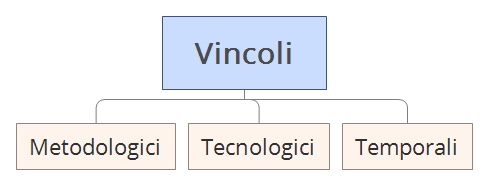
\includegraphics[scale=0.5]{immagini/vincoli}
%			\caption{Vincoli del progetto}
%		\end{figure}
%	
%	\subsubsection*{Metodologici}
%		La prima tipologia di vincoli a cui il progetto era sottoposto erano i vincoli metodologici.
%		
%		
%		Con il \textit{tutor} aziendale abbiamo stabilito che il lavoro doveva essere svolto presso la sede aziendale, per avere miglior approccio e comunicazione con il \textit{tutor} stesso e gli altri colleghi. L'azienda ha posto questo vincolo anche per cercare raggiungere l'obiettivo di prospettiva di assunzione descritto nella sezione \ref{sec:motivazioni_aziendali}.
%		
%		
%		Un altro vincolo stabilito riguardava l'interazione con il \textit{tutor} e la richiesta di informazioni tecniche ai colleghi. Dati i frequenti impegni del \textit{tutor}, nel caso di necessità di informazioni tecniche avrei dovuto chiedere ai colleghi d'ufficio facenti parte del \textit{team} Java 3, senza però abusare di tale possibilità. Uno degli obiettivi che l'azienda ha cercato di raggiungere con questo vincolo è quello di migliorare le mie capacità di \textit{problem solving} e di lavoro in autonomia, insegnandomi a riconoscere i problemi risolvibili da me e quelli che invece necessitano di personale più esperto. I rapporti con il \textit{tutor} si sarebbero dovuti limitare a richieste riguardo i requisiti e a revisioni periodiche per valutare i risultati raggiunti.
%		
%	\subsubsection*{Tecnologici}
%		\label{sec:vincoli-tecnologici}
%		Gli unici vincoli tecnologici imposti dall'azienda riguardavano l'implementazione di esempi di codice e di un prototipo basato sulla libreria Jackrabbit, utilizzando quindi il linguaggio Java.
%		
%		
%		Per quanto riguarda il versionamento, IBC ha predisposto un \textit{repository} SVN su cui avrei dovuto effettuare i \textit{commit} di codice e documentazione.
%		
%		
%		Non abbiamo fissato vincoli stretti riguardo la gestione della configurazione, anche se il \textit{tutor} mi ha fortemente consigliato di utilizzare Maven, data l'esperienza positiva che l'azienda ha avuto con tale strumento.
%		
%		
%		La scelta di eventuali \textit{framework} per l'implementazione dell'interfaccia grafica del prototipo era libera, a patto che fosse possibile l'interfacciamento con il JCR offerto da Jackrabbit. Questo mi ha portato a dover effettuare una scelta:
%		\begin{itemize}
%			\item La prima opzione che ho considerato è stato l'utilizzo del linguaggio PHP, da me già conosciuto. Ho presto realizzato che per percorrere questa strada avrei dovuto utilizzare la libreria Jackalope, che fornisce un'implementazione di JCR accessibile tramite API PHP. Nonostante la presenza di Jackalope-Jackrabbit, un'implementazione basata sul JCR fornito da \gls{jackrabbit}, ho trovato questa soluzione troppo complicata e scarsamente documentata.
%			\item La seconda opzione che ho considerato è stato JavaServer Faces (JSF), un \textit{framework} Java basato sul \textit{design pattern} MVC per lo sviluppo di applicazioni \textit{web}. Dopo aver letto varie opinioni \textit{online}, ho scartato questa scelta in quanto risulta essere molto complicata. Uno dei motivi principali di questa complessità è, come citato da ThoughtWorks nell'articolo raggiungibile al link \url{https://goo.gl/dfxpaC}, \jquote{pensiamo che [JSF] sia imperfetto in quanto tenta di astrarre troppo l'HTML, il CSS e l'HTTP}.
%			\item La terza opzione, quella da me scelta, è stato Apache Wicket, anch'esso un \textit{framework} Java che utilizza MVC con la caratteristica aggiuntiva di essere basato su componenti. Questa caratteristica, unita al fatto che Wicket permetteva l'interfacciamento senza alcuna complicazione al JCR e che era utilizzato anche da IBC, mi hanno portato a preferirlo alle altre tecnologie.
%		\end{itemize}
%		Alla luce di questa e altre decisioni, includo una tabella che elenca le tecnologie utilizzate durante il progetto.
%		
%		\begin{table}[H]
%			\centering
%			\begin{tabularx}{\textwidth}{|X | X | X |}
%				\hline
%				\rowcolor{lightgray}
%			  \textbf{Documentazione} & 	\textbf{{Config.} e \mbox{versionamento}}  &  \textbf{Sviluppo} \\
%				\hline
%				 LibreOffice & Maven & Eclipse \\
%				\hline
%				 & SVN & Jackrabbit \\
%				\hline
%				 & Tomcat & Wicket \\
%				\hline
%				& & Wicket-Bootstrap \\
%				\hline
%				& & JUnit \\
%				\hline
%			\end{tabularx}
%			\caption{Principali tecnologie utilizzate nel progetto.}
%		\end{table}
%	
%	\subsubsection*{Temporali}
%		Per quanto riguarda i vincoli temporali, gli orari di lavoro erano gli stessi del personale IBC, ovvero dal Lunedì al Venerdì con orario dalle 8:30 alle 12:30 e dalle 14:00 alle 18:00. L'azienda non ha richiesto moduli o procedure particolari per l'assenza da lavoro o la variazione di orario per motivi universitari, tranne la comunicazione a voce al \textit{tutor} o ad un collega.
%		
%		
%	\subsection{Pianificazione del lavoro}
%		La pianificazione del lavoro ha dovuto tener conto dei vincoli temporali esposti nella sezione precedente.
%		
%		
%		Ho pianificato lo svolgimento delle attività in otto settimane lavorative da quaranta ore ciascuna, come mostrato nel Gantt sottostante.
%			\begin{figure}[H]
%				\centering
%				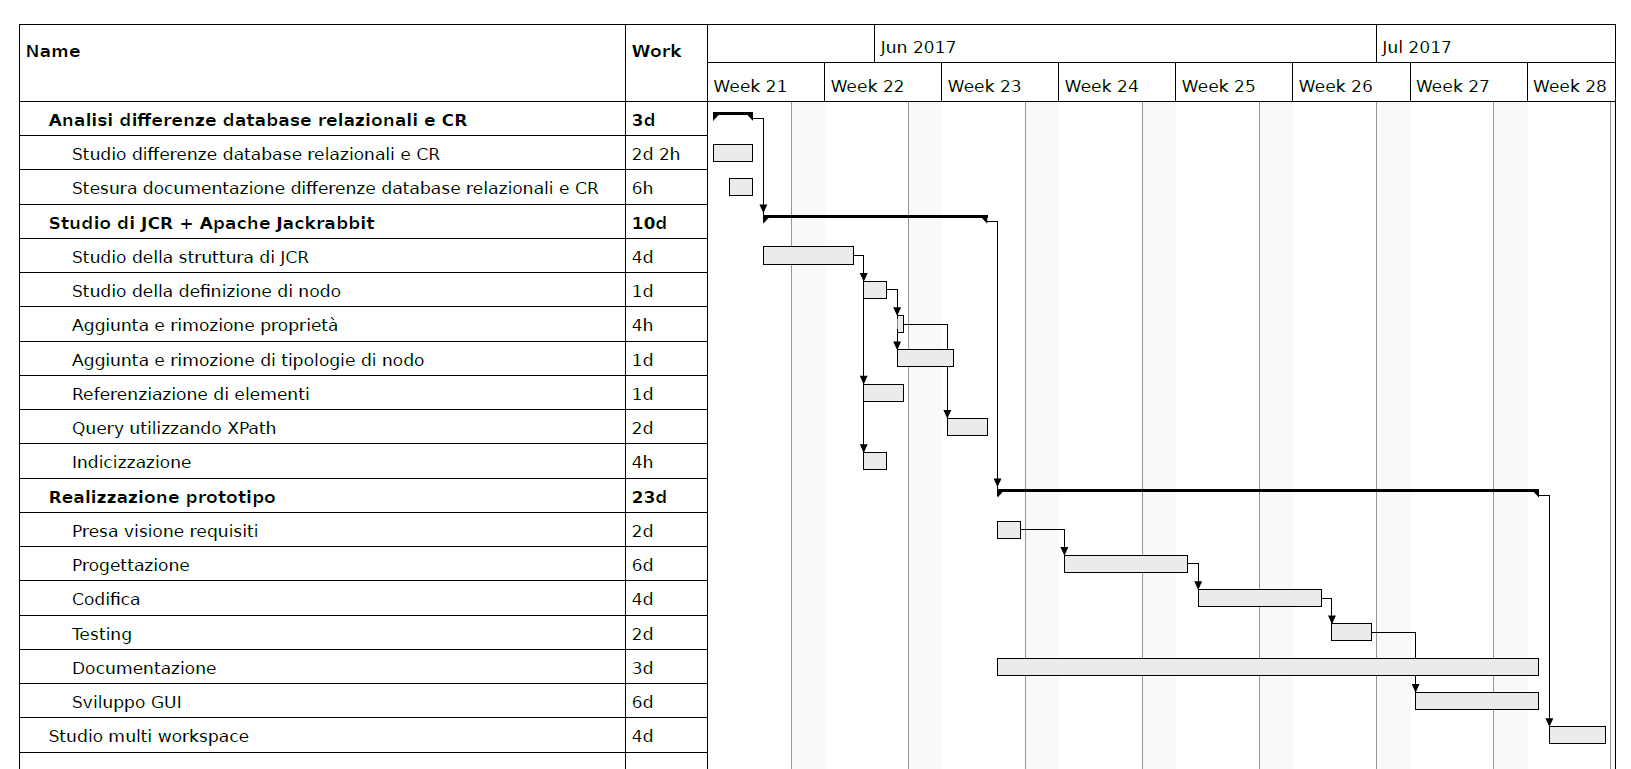
\includegraphics[width=\textwidth]{immagini/gantt-pianificazione}
%				\caption{Pianificazione temporale.}
%			\end{figure}
%		
%		Durante lo svolgimento iniziale delle attività di analisi e studio ho seguito il piano, ma durante la realizzazione del prototipo non ho rispettato la netta sequenzialità tra realizzazione del prototipo e sviluppo della GUI. Il motivo di questa decisione è dovuto al fatto che ho deciso di raggiungere l'obiettivo desiderabile stabilito dal piano di lavoro. Ho avuto quindi la necessità di iniziare ad apprendere il \textit{framework} scelto per l'interfaccia al più presto, portandomi a svolgere le attività di realizzazione della logica del prototipo e della parte grafica in parallelo.
%
%		Tenendo conto di questo punto, il reale svolgimento delle attività è stato il seguente.
%		
%		\begin{figure}[H]
%			\centering
%			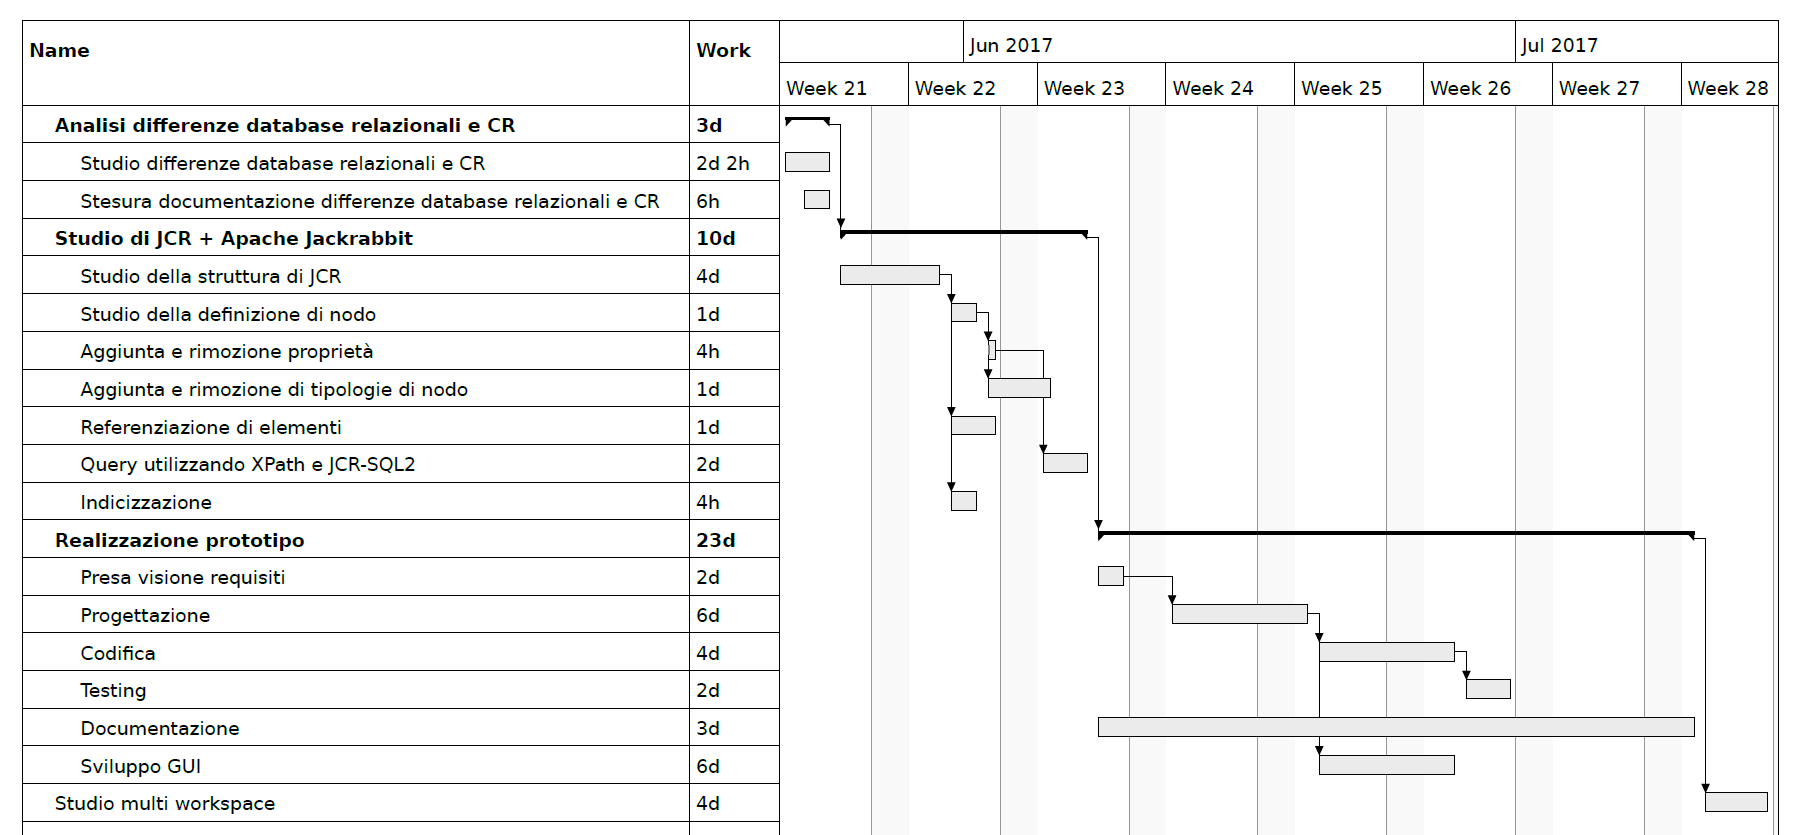
\includegraphics[width=\textwidth]{immagini/gantt-consuntivo}
%			\caption{Svolgimento attività.}
%		\end{figure}
%		
%
%\section{\textit{Stage} in IBC: motivazioni personali}
%	\label{sec:motivazioni_personali}
%	Durante la partecipazione a StageIt ho sostenuto colloqui con undici aziende. La mia scelta è ricaduta su IBC per una serie di motivi suddivisibili in tre tipologie: economici e logistici, professionali, personali.
%	
%	\subsubsection*{Economici e logistici}
%		\begin{itemize}
%			\item L'azienda, al contrario di molte altre, offriva un rimborso spese. Personalmente lo considero come un modo di riconoscere del valore nel lavoro svolto dallo stagista. Inoltre, la gratificazione ricevuta da questo riconoscimento è un buon punto di partenza per un rapporto che potrebbe continuare dopo la fine dello \textit{stage}.
%			\item Il posizionamento del luogo di lavoro, situato a dieci minuti da casa e vicino a Padova, era ideale per permettermi di raggiungere in breve tempo la sede dell'università. Infatti, data la necessità di terminare il progetto didattico di \gls{swe}, ho dovuto presenziare ad alcuni incontri con i miei compagni di progetto dopo l'orario di lavoro. Un'azienda situata più lontano non mi avrebbe permesso tale flessibilità.
%		\end{itemize}
%	
%	\subsubsection*{Professionali}
%		\begin{itemize}
%			\item IBC è un'azienda che non si occupa solamente di consulenza, ma produce anche \textit{software} proprio. Svolgere lo \textit{stage} presso IBC mi ha permesso di essere immerso in un ambiente che unisce entrambe le realtà.
%			\item Data la diffusione del linguaggio Java in ambito aziendale, ho valutato positivamente un'esperienza in una realtà che, oltre ad usare tale linguaggio, produce applicazioni che si basano su \gls{javaee}.
%		\end{itemize}
%	
%	\subsubsection*{Personali}
%	\begin{itemize}
%		\item Con questo \textit{stage} ho voluto valutare se l'impiego presso un'azienda che produce \textit{software} fosse adatto a me. Inoltre, dato che questa sarebbe stata la mia prima esperienza lavorativa, mi sono posto come obiettivo quello di rapportarmi con il personale esperto per avere consigli ed informazioni su come gestire un lavoro in campo informatico.
%	\end{itemize}
%
%%**************************************************************
%%\chapter{L'azienda}
%%\label{cap:lazienda}
%%%**************************************************************
%%
%%Introduzione al contesto applicativo.\\
%%
%%\noindent Esempio di utilizzo di un termine nel glossario \\
%%\gls{api}. \\
%%
%%\noindent Esempio di citazione in linea \\
%%\cite{site:agile-manifesto}. \\
%%
%%\noindent Esempio di citazione nel pie' di pagina \\
%%citazione\footcite{womak:lean-thinking} \\
%%
%%%**************************************************************
%%\section{L'azienda}
%%
%%Descrizione dell'azienda.
%%
%%%**************************************************************
%%\section{L'idea}
%%
%%Introduzione all'idea dello stage.
%%
%%%**************************************************************
%%\section{Organizzazione del testo}
%%
%%\begin{description}
%%    \item[{\hyperref[cap:processi-metodologie]{Il secondo capitolo}}] descrive ...
%%    
%%    \item[{\hyperref[cap:descrizione-stage]{Il terzo capitolo}}] approfondisce ...
%%    
%%    \item[{\hyperref[cap:analisi-requisiti]{Il quarto capitolo}}] approfondisce ...
%%    
%%    \item[{\hyperref[cap:progettazione-codifica]{Il quinto capitolo}}] approfondisce ...
%%    
%%    \item[{\hyperref[cap:verifica-validazione]{Il sesto capitolo}}] approfondisce ...
%%    
%%    \item[{\hyperref[cap:conclusioni]{Nel settimo capitolo}}] descrive ...
%%\end{description}
%%
%%Riguardo la stesura del testo, relativamente al documento sono state adottate le seguenti convenzioni tipografiche:
%%\begin{itemize}
%%	\item gli acronimi, le abbreviazioni e i termini ambigui o di uso non comune menzionati vengono definiti nel glossario, situato alla fine del presente documento;
%%	\item per la prima occorrenza dei termini riportati nel glossario viene utilizzata la seguente nomenclatura: \emph{parola}\glsfirstoccur;
%%	\item i termini in lingua straniera o facenti parti del gergo tecnico sono evidenziati con il carattere \emph{corsivo}.
%%\end{itemize}         
% !TEX encoding = UTF-8
% !TEX TS-program = pdflatex
% !TEX root = ../tesi.tex

\chapter{ROFF}
\label{chapter:roff}

	RObust and Fast Forwarding scheme (ROFF) is a protocol proposed by Hongseok Yoo and Dongkyun Kim in \cite{6906275}. This chapter will present the two main problems tackled by ROFF already introduced in Section \ref{sec:emd}, namely the perfect suppression of redundant transmissions, which will be explained in \ref{ssec:collision-analysis} , and the disuniformity and the costant change in spatial vehicle distribution in VANETs, addressed in section \ref{ssec:latency-analysis}.

	\section{Forwarder Selection Problem}
		\subsection{Collision Analysis}
			\label{ssec:collision-analysis}
			The first problem tackled by ROFF concerns collisions caused by nodes who start to transmit at the same time. This results in a collision in the area resulting from the intersection of the nodes' transmission ranges.
			
			
			Suppose that $S_f=\{f_i | 0 < i \leq N, i \in \mathbb{N} \}$ is the set of PFCs ordered in ascending order by the distance between the previous forwarder and the PFC, where N is the number of PFCs and $f_n$ is the FFC. We define $f_0$ as the previous forwarder.
			%TODO immagine con 1..n PFC
			Based on the most common idea in existing protocols, ideally a PFC $f_i$ suppresses its scheduled transmission whenever it receives the transmission from $f_N$. In order to achieve suppression, vehicles from $f_i$ to $f_i-1$ should wait until they receive the transmission from $f_N$ before forwarding. If a vehicle forwards the message before having received the transmission from $f_N$, then a collision will occur. As stated in Section \ref{sec:emd}, existing protocols employ a strategy for waiting time assignment by which each PFC calculates its waiting time based on the distance between itself and the previous forwarder (that is $distance = d(f_i, f_0)$). As a consequence, successful suppression of all PFCs ($f_1$ to $f_{N-1}$, $f_{N-1}$ included) can be achieved only if the timer of $f_{N-1}$ is long enough to detect the transmission from $f_N$. The authors define $minDiff$ as the minimum time difference between $f_N$ and $f_{N-1}$ to prevent $f_{N-1}$ from forwarding.
			
			\begin{figure}[H]
				\centering
				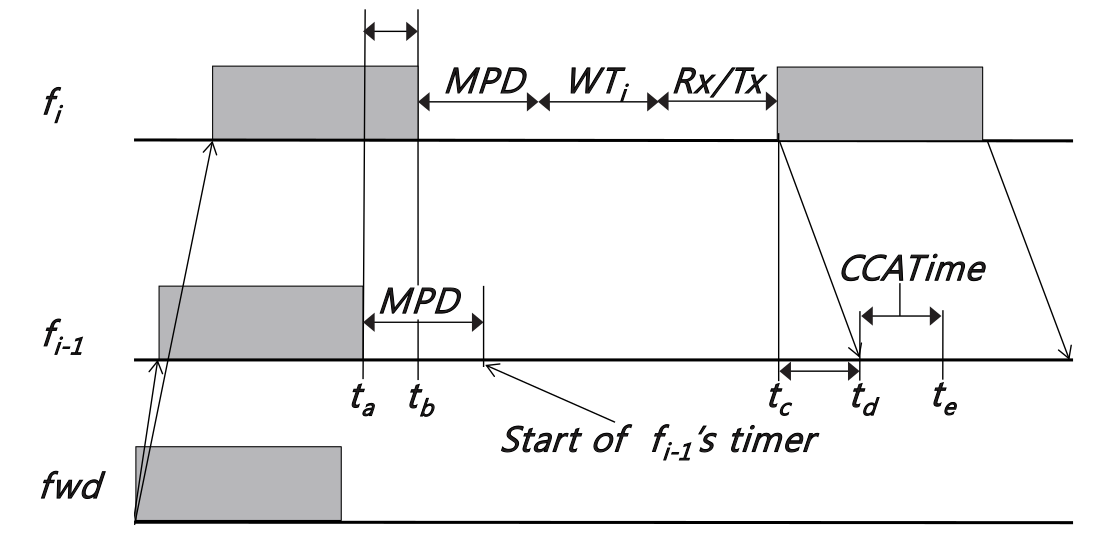
\includegraphics[width=\textwidth]{immagini/minDiff}
				\caption{Definition of $minDiff$ between $f_N$ and $f_{N-1}$ (\cite{6906275})}
				\label{fig:minDiff}
			\end{figure}
		
			\imgrefcap{fig:minDiff} depicts a situation where $fwd$ is the forwarder and $f_i$ (farther from fwd than $f_{i-1}$) relays the message before $f_{i-1}$. The two vehicles $f_i$ and $f_{i-1}$ complete receiving the message at different times ($t_a$ and $t_b$) due to propagation delay (calculated as $pd = d / s$, where $d$ is the distance between two points in space and $s$ is the wave propagation speed of the medium, i.e. $s=c$, the speed of light, in wireless communication). After reception we have additional amount of time in order to process and retransmit the message:
			\begin{itemize}
				\item Each PFC spends MAC Processing Delay (MPD) to process the message and then waits for $WT_i$ calculated according to whichever multi-hop algoritm is being used. As explained previously, this waiting time is inversely proportional to the distance between the PFC and $fwd$;
				\item After timer expiration, each PFC wait for Rx/Tx turnaround time ($Rx/Tx$), in order to switch their interface from reception to transmission mode.
			\end{itemize}
			After $f_i$ has forwarded the message, $f_{i-1}$ starts receiving it at $t_d$, $t_d-t_c$  being equal to $pd{f_{i-1}, f_i}$. The time between the PHY module of $f_{i-1}$ starts reception and the MAC module of the same vehicle is aware of reception is called $CCATime$. Hence, if $f_{i-1}$'s timer expires between $t_a$ and $t_e$, $f_{i-1}$'s transmission will collide with $f_i$'s. In order to accomplish succesful suppression, $f_{i-1}$'s timer should not expire  before $t_e$. 
			
			
			Given the fact that Propagation delay is not controllable and MPD, $Rx/Tx$ and $CCATime$ are usually standard-defined parameters, an algorithm can only manage the difference between waiting times of $f_i$ and $f_{i-1}$ (represented by $WT_i$ and $WT_{i-1}$ respectively in the following formula).
			To achieve succesful suppression, $f_{i-1}$ should wait until the forwarding from $f_i$ is detected by $f_{i-1}$ MAC layer, so $MPD+WT_{i-1}$ should be greater than $t_e - t_a$. Hence, $minDiff = (pd_{fwd, f_i} - pd_{fwd, f_{i-1}}) + pd_{f_i, f_{i-1}} + Rx/Tx + CCATime$.
		
		\subsection{Latency Analysis}
			\label{ssec:latency-analysis}
			The second problem ROFF tries to overcome is the effect of empty space in vehicle distribution on forwarding latency.
			
			The region where PFCs are placed can be defined as \textit{naive forwarding area} (NFA) and is defined as the intersection between:
			\begin{itemize}
				\item the transmission range of a forwarder $fwd$;
				\item the area in the opposite movement direction of the same forwarder $fwd$.
			\end{itemize}
			The distribution of vehicle inside NFA can vary in time; moreover, vehicles are not usually placed at the same distance, so empty spaces of various sizes exist inside the area.
			
			\begin{figure}[H]
				\centering
				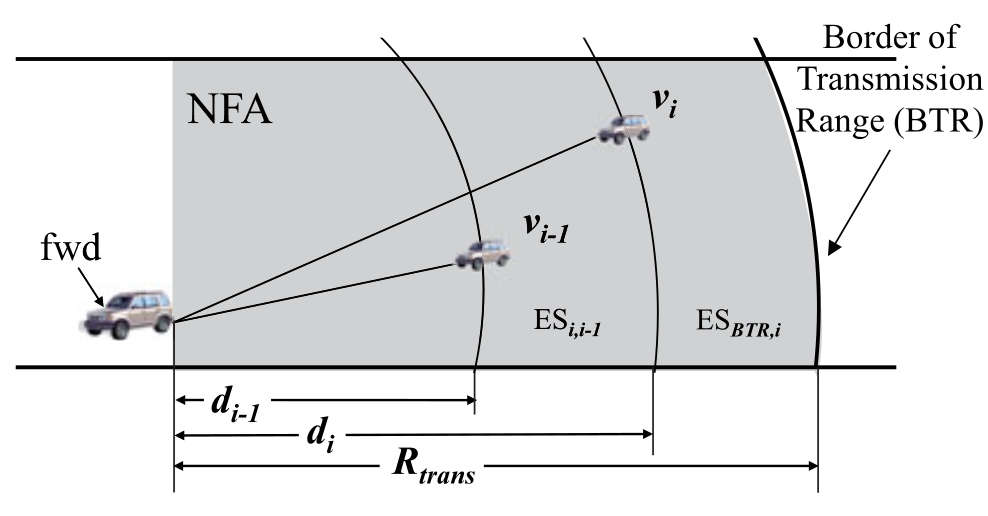
\includegraphics[width=\textwidth]{immagini/emptySpace}
				\caption{Definition of empty space (\cite{6906275})}
				\label{fig:emptySpace}
			\end{figure}
			
			Suppose that $S_v = \{v_i | 0 < i \leq M\}$ is a set of M vehicles inside NFA with vehicles ordered by distance between the vehicle and the previous forwarder in ascending order. Referring to Figure \ref{fig:emptySpace} , the empty space $ES_i,i-1$ between $v_i$ and $v_{i-1}$ is the segment within the two circles centered in $fwd$ with radius $d_{i-1}$ and $d_i$ respectively. Hence, the size of $ES_i,i-1$ is equal to $d_i - d{i-1}$.
			
			
			Large empty spaces have a negative effect on forwarding latency. There is no guarantee that the farthest vehicle from the previous forwarder become the FFC: lossy channel environments, shadowing and other phenomena can make any vehicle within NFA become the forwarder. Suppose that $fwd$ is the previous forwarder and there are two vehicles, $A$ and $B$, inside NFA where A is farther from $fwd$ than $B$, $A$ has not received the transmission from $fwd$ while B has. The empty space $ES_A,B$ between $A$ and $B$ influences the forwarding latency:
			\begin{itemize}
				\item if  $ES_A,B$ is small, $B$ relays the message after a short waiting time;
				\item if $ES_A,B$ is large, $B$ waits needlessly (since there is no other vehicle farther from $fwd$ which has received the message) a large amount of time.
			\end{itemize}
			ROFF aims at resolving the effect of empty spaces by allowing vehicles to choose waiting time inversely proportional to their \textit{unique forwarding priority} proportional to the distance between the vehicle and the previous forwarder, instead of using directly such distance in the waiting time computation.
		
	\section{ROFF Algorithm}
		The ROFF algorithm works under the following two assumptions:
		\begin{enumerate}
			\item each vehicle has access to a GPS system and a digital map;
			\item vehicles periodically (e.g. every 100 milliseconds) broadcast a Hello message containing various information, such as its position, velocity, etc. The period between each Hello message broadcast is called \textit{Beacon Interval}.
		\end{enumerate}
		The algorithm is composed of three components, as depicted in Figure \ref{fig:roffAlgo}.
	
		\begin{figure}[H]
			\centering
			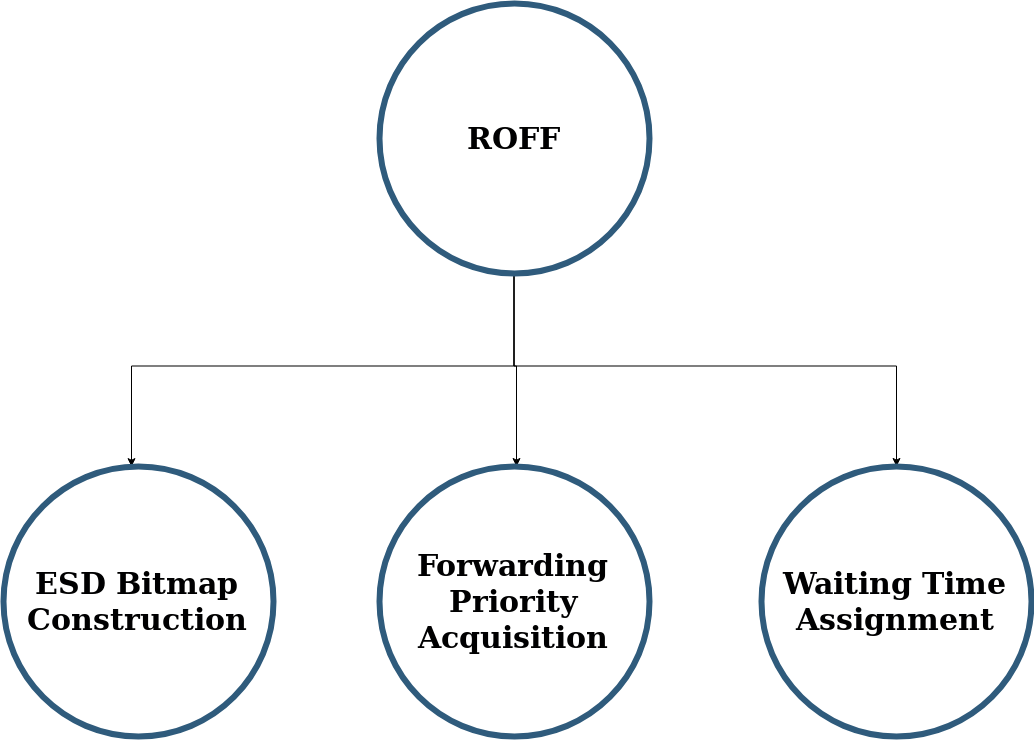
\includegraphics[width=0.7\textwidth]{immagini/roffAlgo}
			\caption{Components of ROFF algorithm}
			\label{fig:roffAlgo}
		\end{figure}
	
		The algorithm in short works as follows (additional information will be given in the following sections):
		\begin{itemize}
			\item when a forwarder relays an Alert Message, it also broadcasts a special structure called ESD Bitmap which describe the empty space distribution within the forwarderś NFA;
			\item PFCs which receive the Alert Message and the ESD Bitmap decide whether they are eligible for contention based on the ESD Bitmap;
			\item Eligible PFCs contend by choosing different waiting times based on a unique forwarding priority.
		\end{itemize}
	
		\subsection{ESD Bitmap Construction}
			Upon Hello Message reception, each vehicle uses the data within the message in order to update and maintain a structure called Neighbor Table (NBT) which monitors its local view (i.e. all the vehicles in the neighborhood of said vehicle). Each entry of the NBT contains:
			\begin{itemize}
				\item the ID of the neighbor;
				\item the position of the neighbor;
				\item the reception time of the Hello Message to verify the freshness of information and remove outdates entries.
			\end{itemize}
			An example of Neighbor Table of node with ID 0 is represented in Picture \ref{fig:nbt}.
				
			\begin{figure}[H]
				\centering
				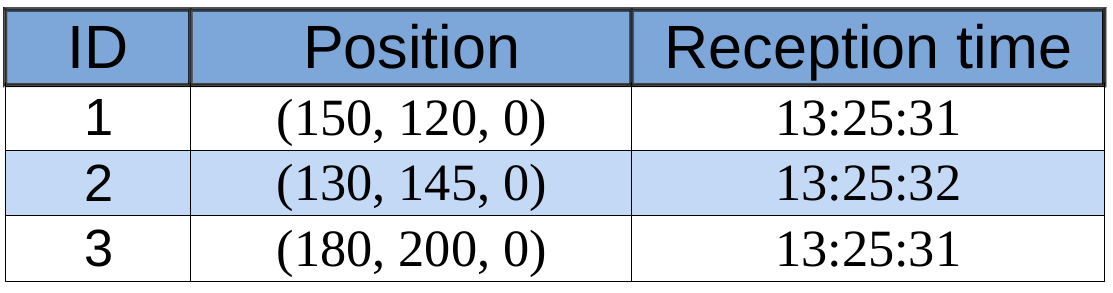
\includegraphics[width=0.7\textwidth]{immagini/nbt}
				\caption{Example of Neighbor Table of node with ID 0}
				\label{fig:nbt}
			\end{figure}
			Thanks to the NBT, the forwarder can advertise its neighborhood to other vehicles. We can define the set of neighbors detected by the forwarder as its \textit{local view}. If a vehicle who receives an Alert Message is not present inside the local view of the forwarder, then that vehicle cannot participate in contention.
			
			
			The NBT could be piggybacked as-is on the Alert Message, but the authors of ROFF identified some problems with this solution, such as the great overhead caused by the size of IDs. Hence, the proposed solution consists in compressing the NBT in a bitmap-like structure called ESD Bitmap. 
			
			
			In order to build the ESD Bitmap, first of all the forwarder measures the distance between itself and each of its neighbors listed in the NBT. Due to GPS granularity, distances are expressed at meter-level and can be represented with non-negative integers.
			
			\begin{figure}[H]
				\centering
				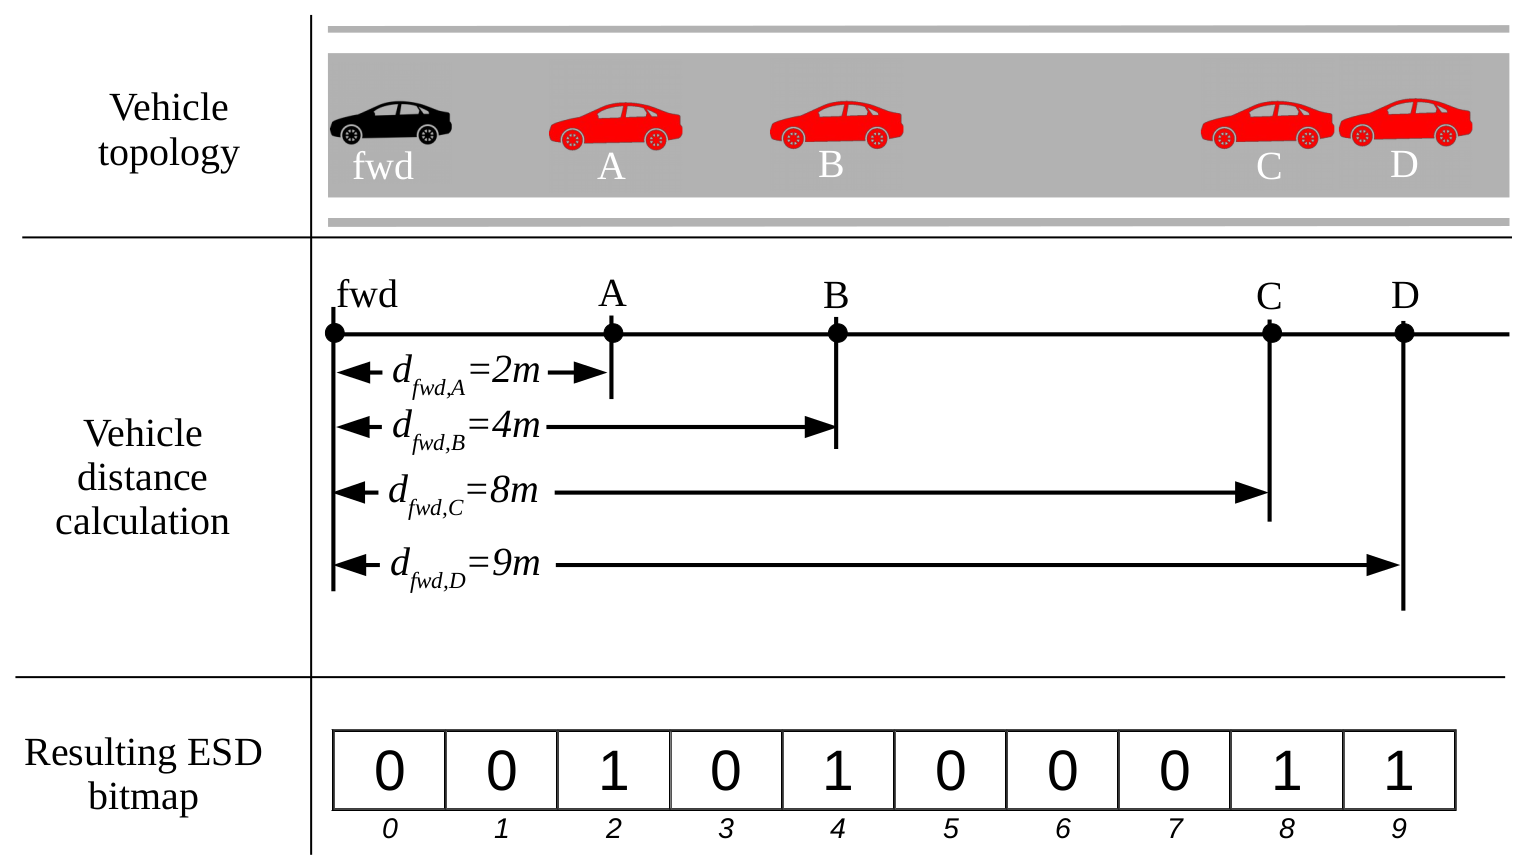
\includegraphics[width=\textwidth]{immagini/esdBitmapConstruction}
				\caption{ESD Bitmap construction with \textit{k} = 1}
				\label{fig:esdBitmapConstruction}
			\end{figure}
			
			After distance measurement, \textit{fwd} builds a bitmap to represent the measured distances by setting the \textit{i-th} bit to either:
			\begin{itemize}
				\item 1 if there is a PFC distant $d$ from \textit{fwd} such that $k * i \leq d \leq k * ( i + 1 ) - 1$;
				\item 0 otherwise.
			\end{itemize} 
			The parameter \textit{k}, called \textit{distance range}, identifies how many distances can be identified by the same bit in the ESD Bitmap. This parameter can be controlled to manage the compression level and the accuracy of the Bitmap. Increasing \textit{k} decreases the number of bits of the Bitmap, but every bit will identify \textit{k} different distances, hence losing precision.
			Picture \ref{fig:esdBitmapConstruction} shows the construction of an ESD Bitmap using $k = 1$.
			
			
			An ESD Bitmap using $k = 2$ is show in Figure \ref{fig:esdBitmapConstructionK2}. It is possible to see that the bit in position 4 represents distances $d$ such that $8 \leq d \leq 9$. 
			
			\begin{figure}[H]
				\centering
				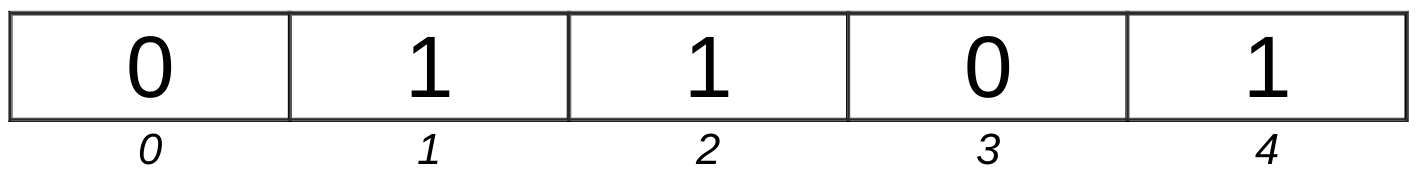
\includegraphics[width=\textwidth]{immagini/esdBitmapConstructionK2}
				\caption{Resulting ESD Bitmap with \textit{k} = 2}
				\label{fig:esdBitmapConstructionK2}
			\end{figure}
		
		\subsection{Forwarding Priority Acquisition}
			Whenever a PFC $f_i$ receives the Alert Message with included the ESD Bitmap from $fwd$, it checks whether the distance between itself and the previous forwarder is listed inside the bitmap (i.e. $f_i$ checks whether the bit in position $d(fwd, f_i)$ in the bitmap is equal to 1, assuming $k = 1$). If so, $f_i$ can participate in contention since it is inside the \textit{local view} of $fwd$. Otherwise, is cannot participate in contention to forward the Alert Message.
			
			
			After $f_i$ has entered contention, it can calculate its own forwarding priority based on the distances express by the ESD Bitmap. These distances are the distances of every other PFC which can participate in contention. Assuming that $L_{dist}$ is the list of distances ordered in ascending order and $distance = d(fwd, f_i)$, $f_i$'s forwarding priority is set as the rank of $distance$ inside $L_{dist}$. This way PFCs that are farther away from $fwd$ are assigned a higher forwarding priority, while PFCs nearer $fwd$ are assigned a lower forwarding priority.
			
			
			ROFF avoids assigning the same priority to two different PFCs by a technique called \textit{ID-based contention}. Using this technique, whenever a PFC $f_i$ receives an Alert Message it checks whether its NBT contains another vehicle $f_j$ whose distance from $fwd$ is the same as $f_i$'s (hence the distance is identified by the same bit in the bitmap). If so, $f_i$ participates in detection only if its ID is higher than the ID of $f_j$. In other words, if inside $f_i$'s NBT there exists an entry for $f_j$ such that $d(fwd, f_i) = d(fwd, f_j)$ and $ID_{f_j} > ID_{f_i}$, then $f_i$ defers its transmission. Figure \ref{fig:idBasedContention} depicts a scenario where node A does not participate in contention due to ID-based contention.
	
			\begin{figure}[H]
				\centering
				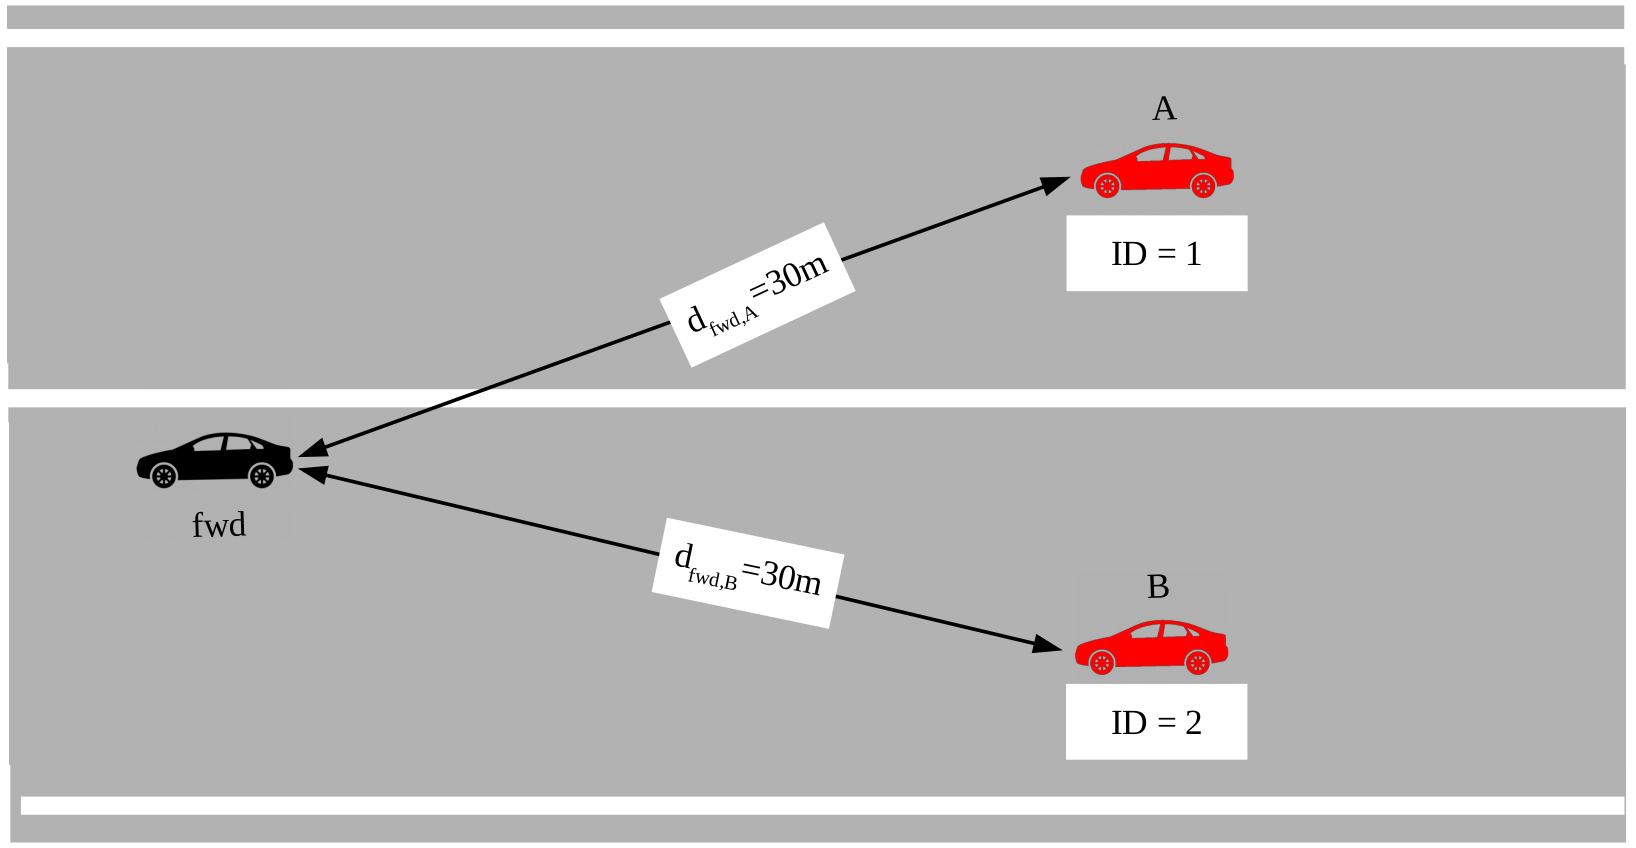
\includegraphics[width=\textwidth]{immagini/idBasedContention}
				\caption{ID-based contention: node A defers its transmission}
				\label{fig:idBasedContention}
			\end{figure}
		
		\section{Waiting Time Assignment}
			Once forwarding priorities are determined, ROFF assigns a waiting time that is inversely proportional to it. Letting $PFC(i)$ be the PFC with forwarding priority $i$ and $WT_p$ the waiting time of PFC $p$, in order to achieve successful suppression of transmission by $PFC(i-1)$, the waiting time of $PFC(i-1)$ should be at least longer by $minDiff_{PFC(i), PFC(i-1)}$ than waiting time of $PFC(i)$ (i.e. $WT_{PFC(i-1)} \geq WT_{PFC(i)} + minDiff_{PFC(i), PFC(i-1)})$. Hence, the waiting time of $PFC(k)$ is the sum of $minDiff$s between PFCs with forwarding priorities lower than $k$, as shown in Equation xxx. PFC with top priority (being equal to 1) broadcasts immediately and does not have to wait any time.
			
			$$WT_{PFC(k)} = \sum_{i=2}^{k} minDiff_{PFC(i),PFC(i-1)} (k \geq 2)$$
		
		
		
		
	      
% !TEX encoding = UTF-8
% !TEX TS-program = pdflatex
% !TEX root = ../tesi.tex


\chapter{Tools and applications}
	\section{Network Simulator 3}
	Network Simulator 3 (ns-3) is a discrete-event network simulator for Internet systems, targeted primarily for research and educational use. ns-3 is free software, licensed under the GNU GPLv2 license, and is publicly available for research, development, and use.
	
	
	ns-3 development began in 2006 by a team lead by Tom Henderson, George Riley, Sally Floyd and Sumit Roy. Its first version was released on June 30, 2008. 
	
	
	ns-3 is the successor of ns-2, released in 1989. The fact that the former was built from scratch makes it impossible to have backward compatibility. In fact, ns-2 used oTCL scripting language to describe network topologies and C++ to write the core of the simulation. This choice was due to avoid the very time consuming C++ code recompilation, exploiting the interpreted language oTCL. ns-2 mixed the \jquote{fast to run, slow to change} C++ with the \jquote{slow to run, fast to change} oTCL language. Since compilation time was not an issue with modern computing capabilities, ns-3 developers chose to utilize exclusively C++ code (and optional Python bindings) to develop simulations.
	
	\subsection{Modules and module structure}
	ns-3 is composed of various modules, which are groups of classes, examples and tests each related to a certain feature. The components of a module work in a cohesive way in order to offer APIs to other modules and users. Some examples of built-in modules are:
	\begin{itemize}
		\item WiFi;
		\item AODV; 
		\item CSMA.
	\end{itemize}
	The obstacle shadowing propagation loss model and the Fast Broadcast algorithm have been implemented as modules too.
	
	
	Modules follow a prototypical structure in order to promote clarity and offer built-in documentation. \imgrefcap{fig:ns-3-module} shows the typical module structure.
	
	\begin{figure}[H]
		\centering
		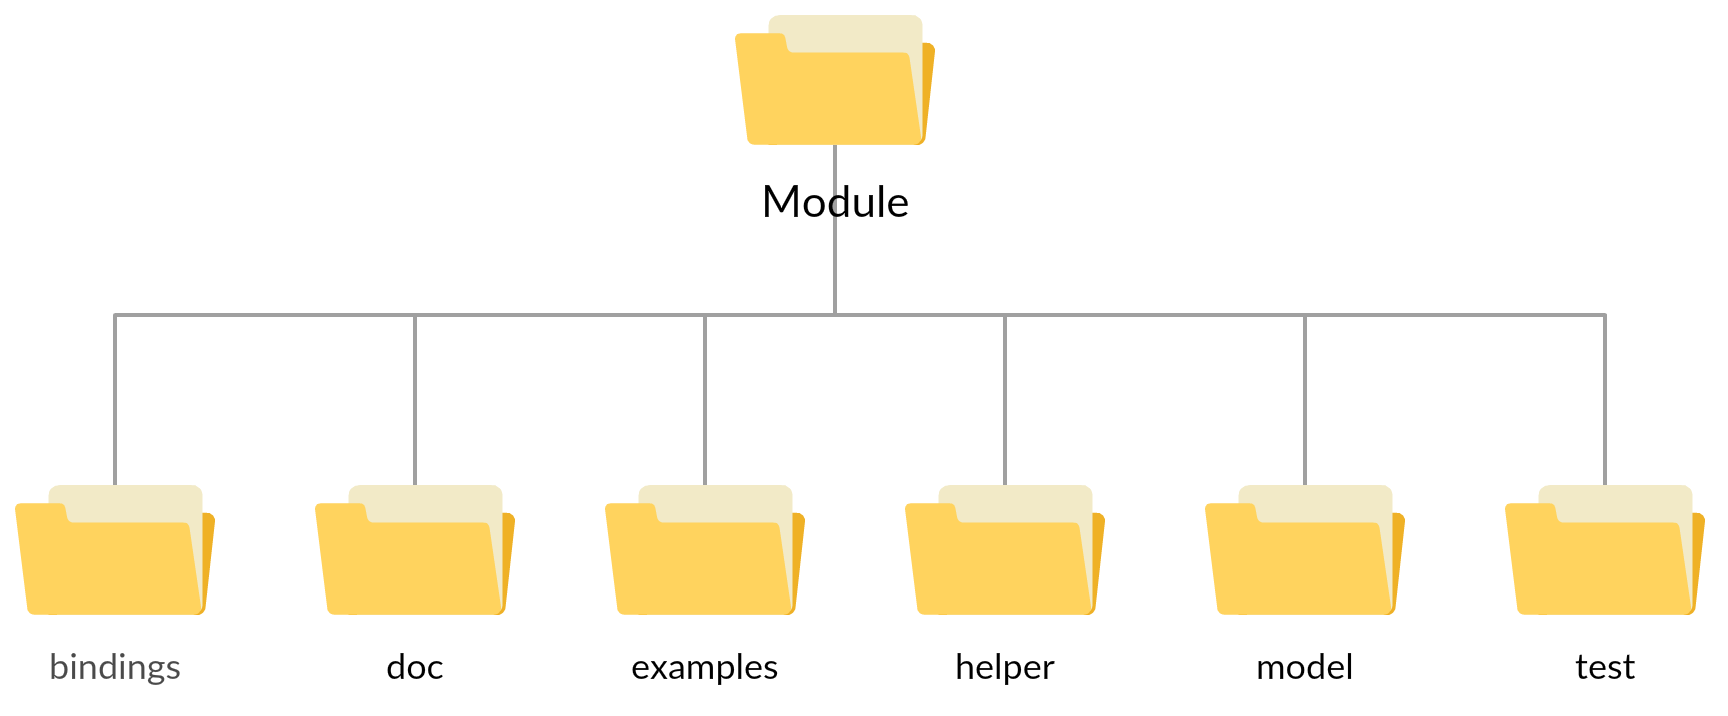
\includegraphics[width=\textwidth]{immagini/ns-3-module}
		\caption{ns-3 module structure}
		\label{fig:ns-3-module}
	\end{figure}
	
	The following directories can be found inside a module's root directory:
	\begin{itemize}
		\item \textbf{bindings:} Python bindings used to make the module's API compatible with Python;
		\item \textbf{doc:} documentation of the module;
		\item \textbf{examples:} examples and proof of concepts of what can be done using the module;
		\item \textbf{helper:} higher level APIs to make the module easier to use;
		\item \textbf{model:} headers and source files which implement the module's logic; 
		\item \textbf{test:} test suite and test cases to test the module.
	\end{itemize}
	
	\subsection{Key elements}
	The element at the base of ns-3 is called \textit{node}, instance of \texttt{ns3::Node}. A node can be thought of as a shell of a computer. Various other elements can be added to nodes, such as:
	\begin{itemize}
		\item NetDevices (e.g. \acrshort{nica}s, which enable nodes to communicate over \textit{channels});
		\item protocols;
		\item applications. 
	\end{itemize}
	The applications implement the logic of a simulation. For example, the \texttt{UdoEchoClientApplication} and \texttt{UdpEchoServerApplication} can be used to implement a client/server application which exchange and print the packets' content over the network. The Fast Broadcast protocol has been implemented as an application as well.
	
	
	The \textit{channels} model various type of transmission media, such as the wired and the wireless ones.
	
	\subsection{Structure of a simulation}
	A simulation can be implemented in many ways, but in most cases the following steps are executed:
	\begin{itemize}
		\item manage command line arguments (e.g. number of nodes to consider in the simulation, transmission range, etc.);
		\item initialize all the necessary fields in classes;
		\item create nodes;
		\item set up physical and MAC layers;
		\item set up link layer, routing protocols and addresses;
		\item configure and install applications on nodes;
		\item position nodes and (optionally) give them a mobility model;
		\item schedule user defined events, such as transmissions of packets;
		\item start the simulation;
		\item collect and manage output data.
	\end{itemize}
	
	\subsection{NetAnim}
	Netanim is an offline animator tool based on the Qt toolkit. It collects an XML tracefile during the execution of a simulation and can be used to animate the simulation, analyzing packet transmissions and contents.
	
	\begin{figure}[H]
		\centering
		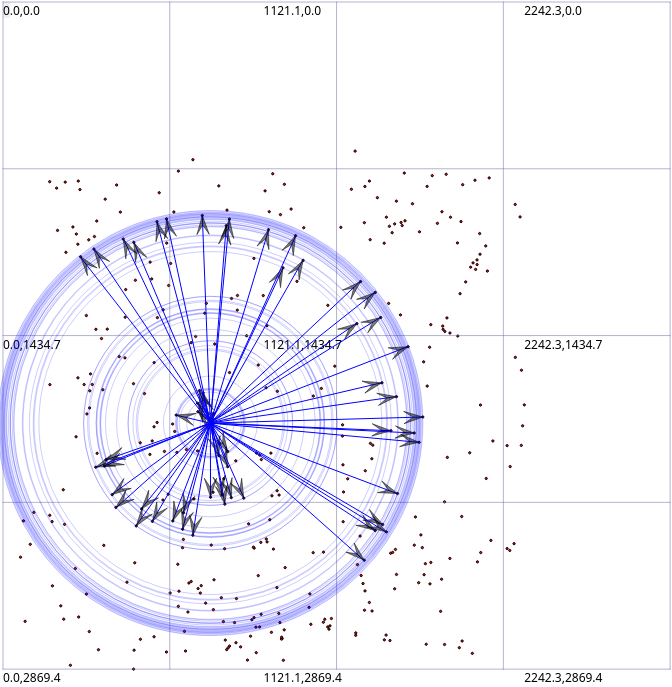
\includegraphics[scale=0.38]{immagini/netanim}
		\caption{Packet transmission in NetAnim}
		\label{fig:netanim}
	\end{figure}
	
	\section{Simulation of Urban MObility}
	Simulation of Urban MObility is an open-source road traffic simulation package. It is written in C++ and licensed under GPLv3. 
	
	
	It offers different tools to analyze and manage real maps from the urban mobility point of view, including pedestrian movement and various types of vehicles.
	
	
	The original work \cite{ROM2017} utilized SUMO to produce, starting from real maps obtained from OpenStreetMap (OSM), two files:
	\begin{enumerate}
		\item a \texttt{.poly} file using the SUMO tool \textit{Polyconvert}. This file contains information about all the obstacles, such as buildings, useful for the Obstacle Shadowing module;
		\item a \texttt{.ns2mobility} file using the SUMO tool \textit{TraceExporter}. This file contains information about the vehicles and their positioning. 
	\end{enumerate}
	The process of generating these two files necessary for ns-3 simulations requires some intermediate steps. The full process is represented in \imgref{fig:sumo-process}. 
	
	The original work considered a only a distance of 25 meters between vehicles; this work considers various distances, ranging from 15 to 45 meters. \imgrefcap{fig:sumo-distances}  shows the same scenario (Padua) with different distances between vehicles.
	
	\begin{figure}[H]
		\centering
		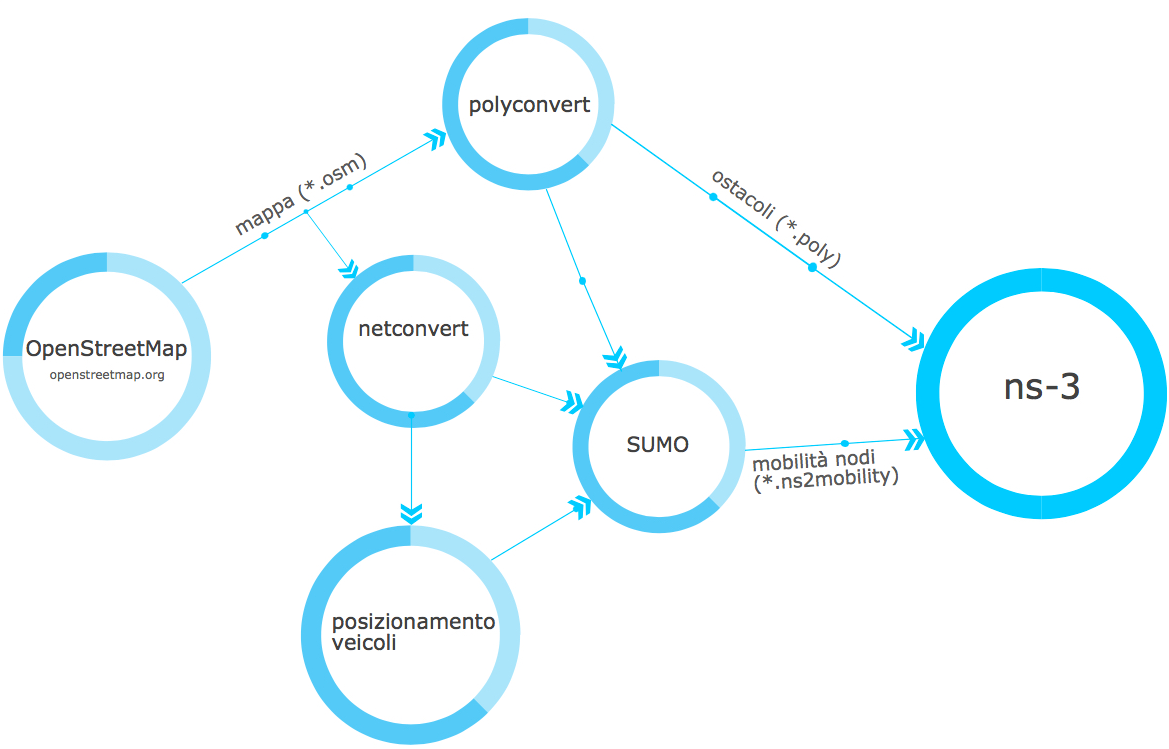
\includegraphics[width=\textwidth]{immagini/sumo-process}
		\caption{Steps to generate necessary files using SUMO (\cite{ROM2017})}
		\label{fig:sumo-process}
	\end{figure}
	
	\begin{figure}[H]
		\centering
		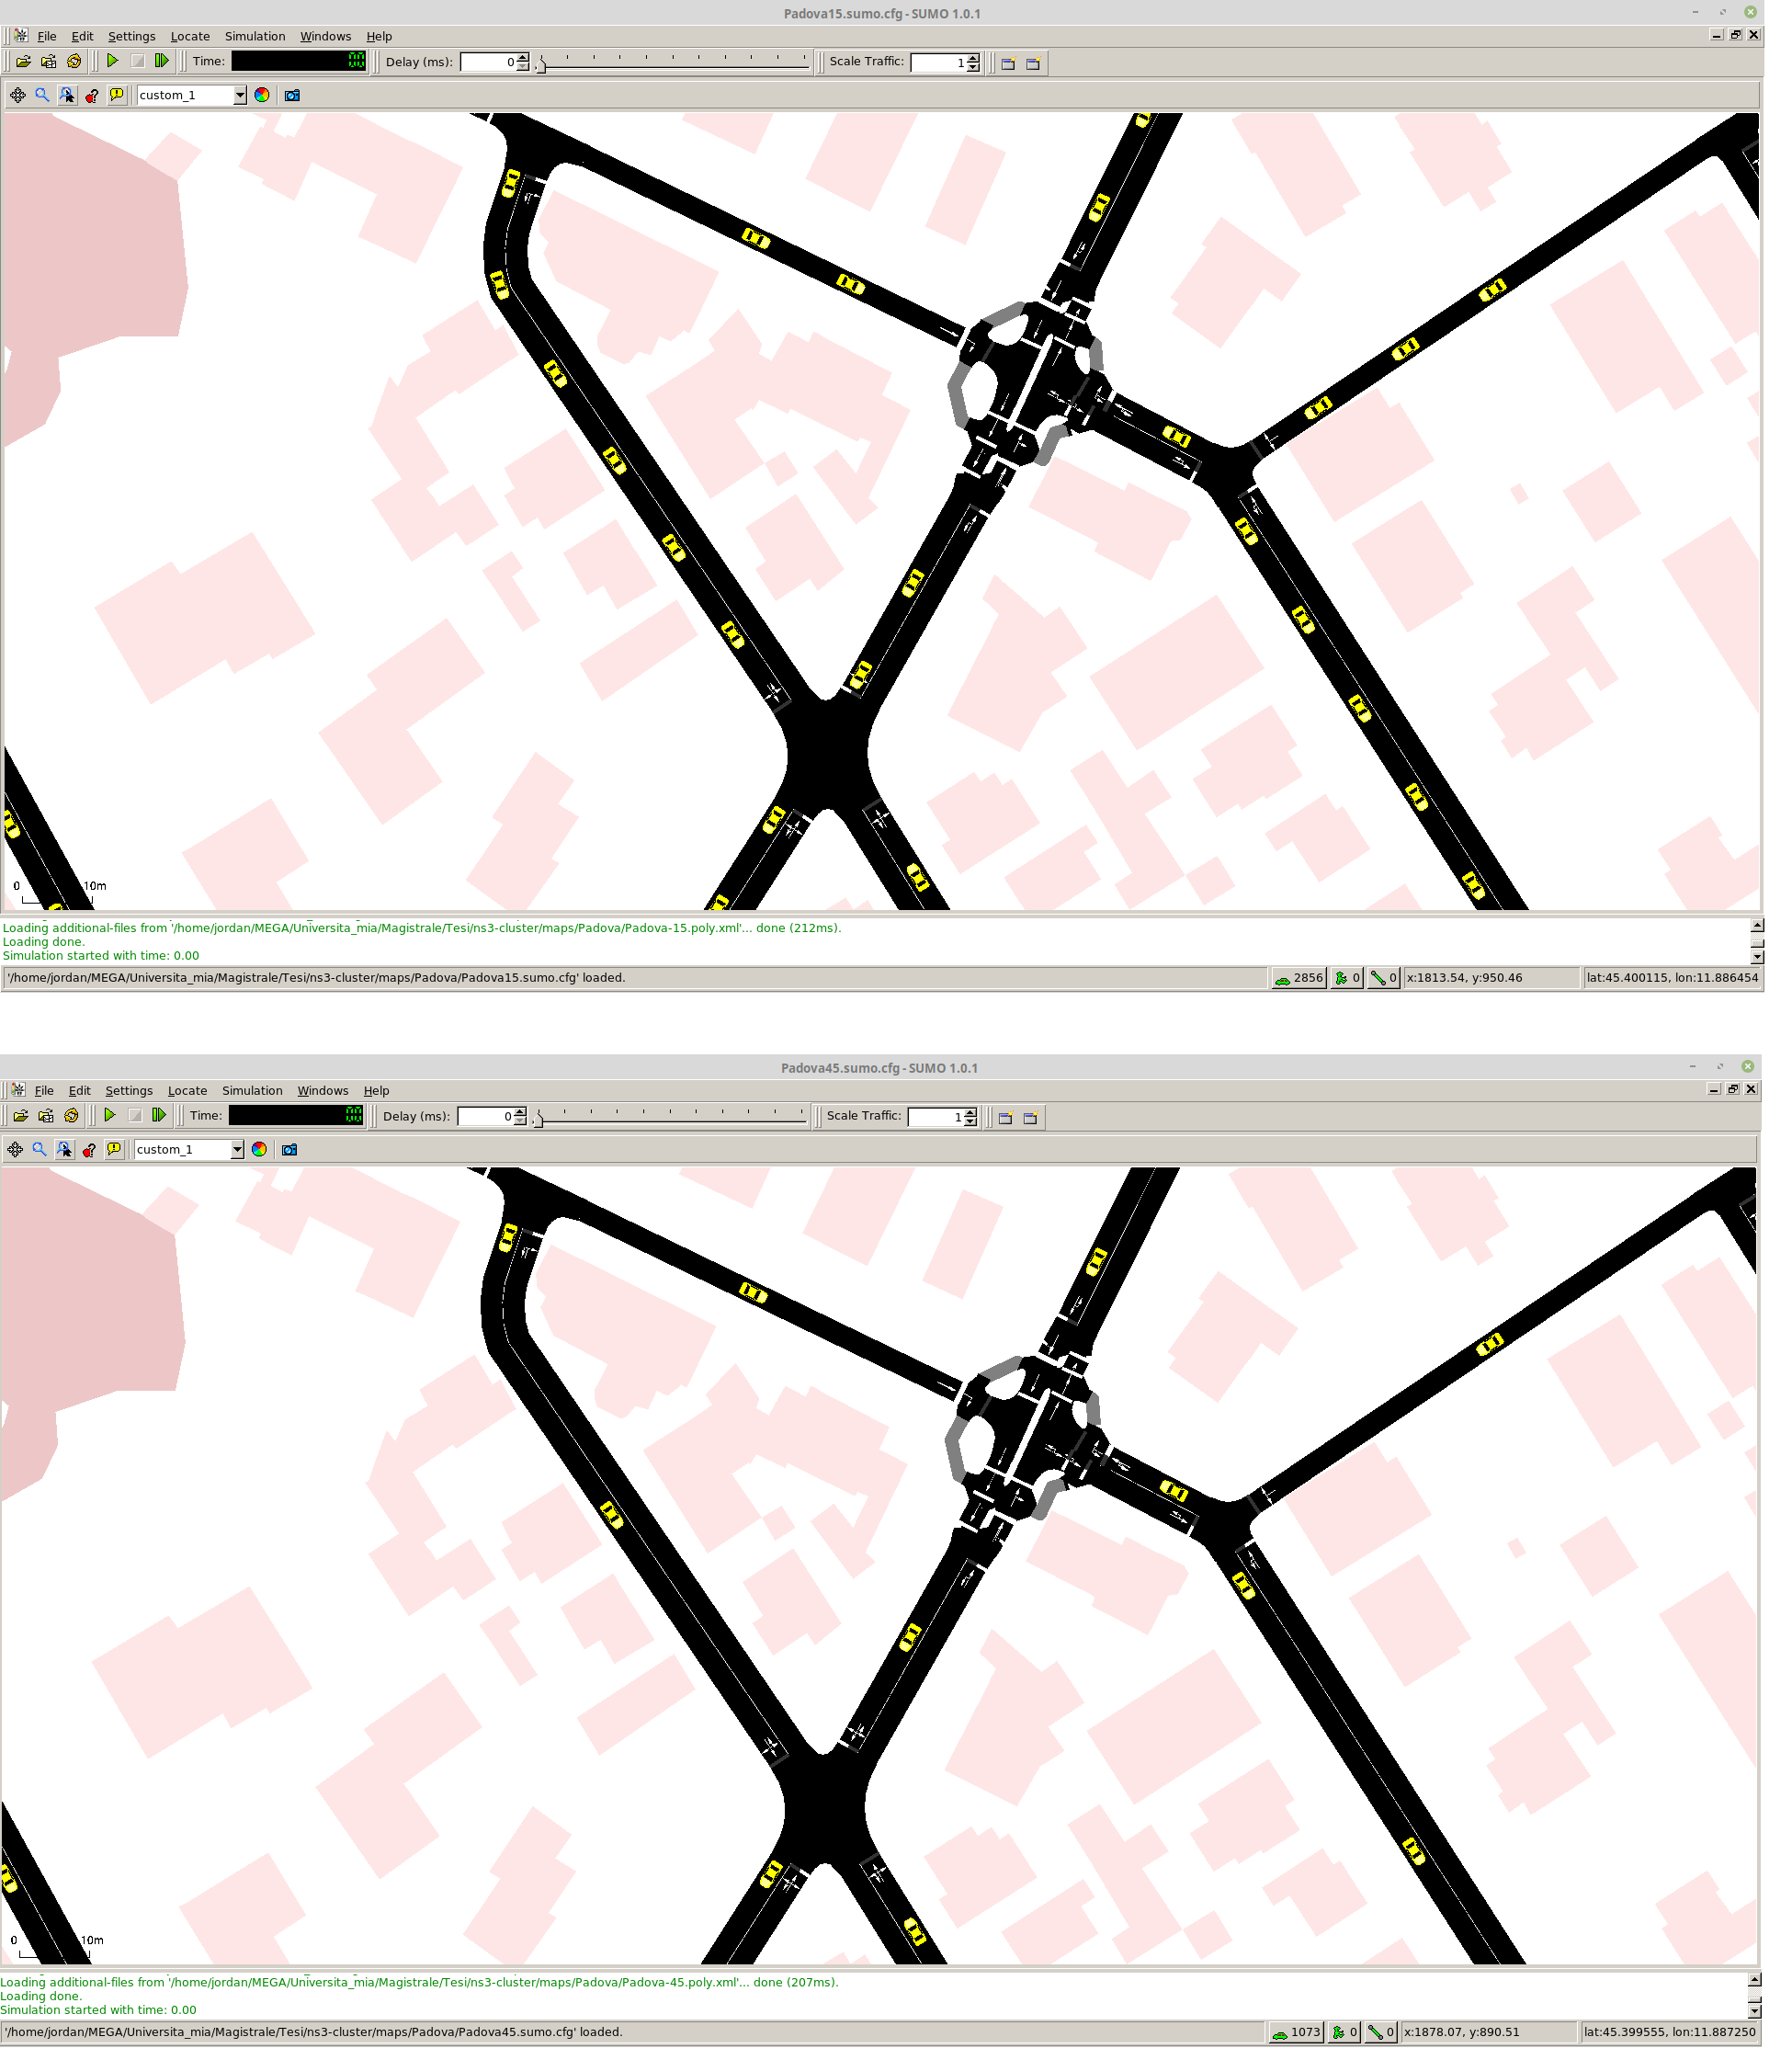
\includegraphics[width=\textwidth]{immagini/sumo-distances}
		\caption{Padua scenario with vehicle distance equals to 15 meters (top) and 45 meters (bottom)}
		\label{fig:sumo-distances}
	\end{figure}
            
% !TEX encoding = UTF-8
% !TEX TS-program = pdflatex
% !TEX root = ../tesi.tex


\chapter{Simulations}
	After the protocols under consideration have been presented in Chapters \ref{chapter:fb} and \ref{chapter:roff}, this Chapter will contain the results of the simulation carried out through various scenario of increasing complexity.
	
	\section{Metrics}
		Before proceeding with the presentation of simulation results, metrics used to evaluate the protocol's performances will be presented in this section. 
		
		\subsection{Total Delivery Ratio (TDR)}
			\label{ssec:tdr}
			This metric is used to detect how many vehicles have received the Alert Message in total. Ideally, broadcasting protocols should be able to reach all the reachable nodes in the scenario in order to warn them of the danger. The metric is calculated as follows:
			
			\begin{gather}
				\label{eq:tdr}
				TDR = \frac{\textrm{\textit{no. of vehicles successfully receiving the Alert Message}}}{\textrm{\textit{no. of vehicles in the scenario}}}
			\end{gather}
			
			All scenarios are created in a way such that every node can be reached by multi-hop propagation regardless of the source of the Alert Message. In other words, from graph theory point of view, the graph resulting from vehicle distribution where two nodes are connected only if they are within transmission range of each other is a connected graph. This way, the term at the denominator of Equation \ref{eq:tdr} is equivalent to the number of vehicles reachable by pure flooding.
			
		\subsection{Total Delivery Ratio On Circumference (TDROC)}
			This metric is used to detect how many vehicles on the circumference have received the Alert Message. The circumference is built starting from the source of the Alert Message. The way it is built depends on scenario topology (e.g. 1D, 2D, etc) and will be explained more thoroughly in the following Sections. The main idea behind the circumference consists in considering only vehicles far from the source of the AM. The metric is calculated as follows:
			
			\begin{gather}
			 	\label{eq:tdroc}
			 	TDROC = \frac{\textrm{\textit{no. of vehicles on circ. successfully receiving the Alert Message}}}{\textrm{\textit{no. of vehicles on circ.}}}
			\end{gather}
		
			The same consideration about vehicles and reachability by pure flooding presented in Section \ref{ssec:tdr} is also valid for Equation \ref{eq:tdroc}.
			
		\subsection{Number Of Hops (NOH)}
			This metric is used to measure the mean number of hops required in order to propagate the Alert Message from the source to all vehicles reached on the circumference. This value is obviously dependent on the paths taken by forwarder Alert Messages from the source to all destinations. We have that \textit{ONOH} is always greater than or equal to the \textit{Optimal Number of Hops BNOH} (i.e. $ONOH \leq NOH$). \textit{BNOH} is calculated using the following formula:
			$$ BNOH = \frac{\textrm{\textit{Circumference Radius}}}{\textrm{\textit{Transmission Range}}} $$
			
			The Number Of Hops metric can be calculated as:
			
			\begin{gather}
				\label{eq:noh}
				NOH = \frac{ \sum_{p \in RC } \textrm{\textit{no. of hops from source to p}}} {\textrm{\textit{no. of vehicles on circ}}}
			\end{gather}
			
			where $RC$ is the set of vehicles which have successfully received the message on the circumference.
			
			
			The \textit{NOH} metric (whose value should be as close as possible to \textit{BNOH} ) is an important indicator of the effectiveness of the multi-hop protocol in choosing the farthest forwarder during contention.
			
			
			Figure \ref{fig:hops} can be used as an example to calculate \textit{NOH}. Using Equation \ref{eq:noh}, the mean number of hops is equal to 3.
			
			\begin{figure}[H]
				\centering
				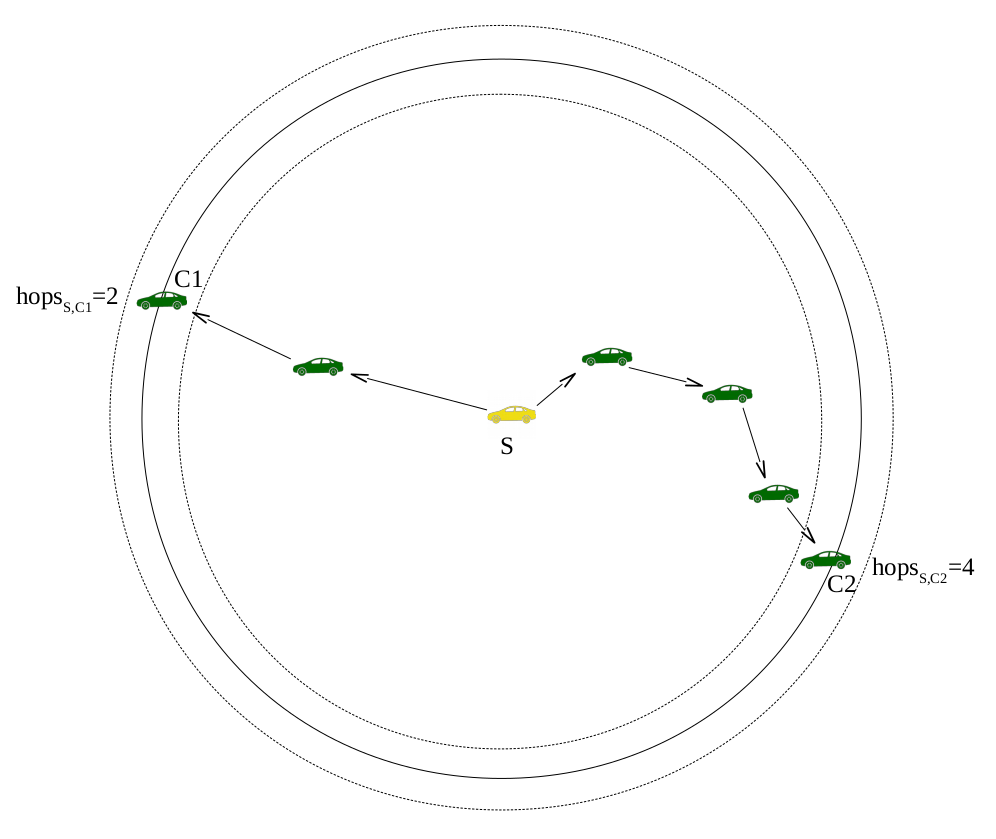
\includegraphics[width=0.7\textwidth]{immagini/hops}
				\caption{Example of \textit{NOH} calculation with Alert Message starting from node S}
				\label{fig:hops}
			\end{figure}
			
		\subsection{Number Of Slots (NOS)}
			This metric is used to measure the number of slots required in order to propagate the Alert Message from the source to all vehicles reached on the circumference. High values of this metric means that the multi-hop protocol introduces a lot of waiting time before each forwarding, hence increasing end-to-end delay and hurting the timeliness of the emergency message propagation.
		
			\begin{gather}
				\label{eq:slots}
				NOH = \frac{ \sum_{p \in RC } \textrm{\textit{no. of slots waited along path from source to p}}} {\textrm{\textit{no. of vehicles on circ}}}
			\end{gather}	
	
			where $RC$ is the set of vehicles which have successfully received the message on the circumference
			The number of slots along the path from node $a$ to $b$ at the numerator of Equation \ref{eq:slots} is the sum of the slots waited by each forwarder before relaying the Alert Message. 
			
			
			Based on the scenario represented in Figure \ref{fig:slots} and Equation \ref{eq:slots}, the mean number of slots from source S to nodes on the circumference is 100.
			
			\begin{figure}[H]
				\centering
				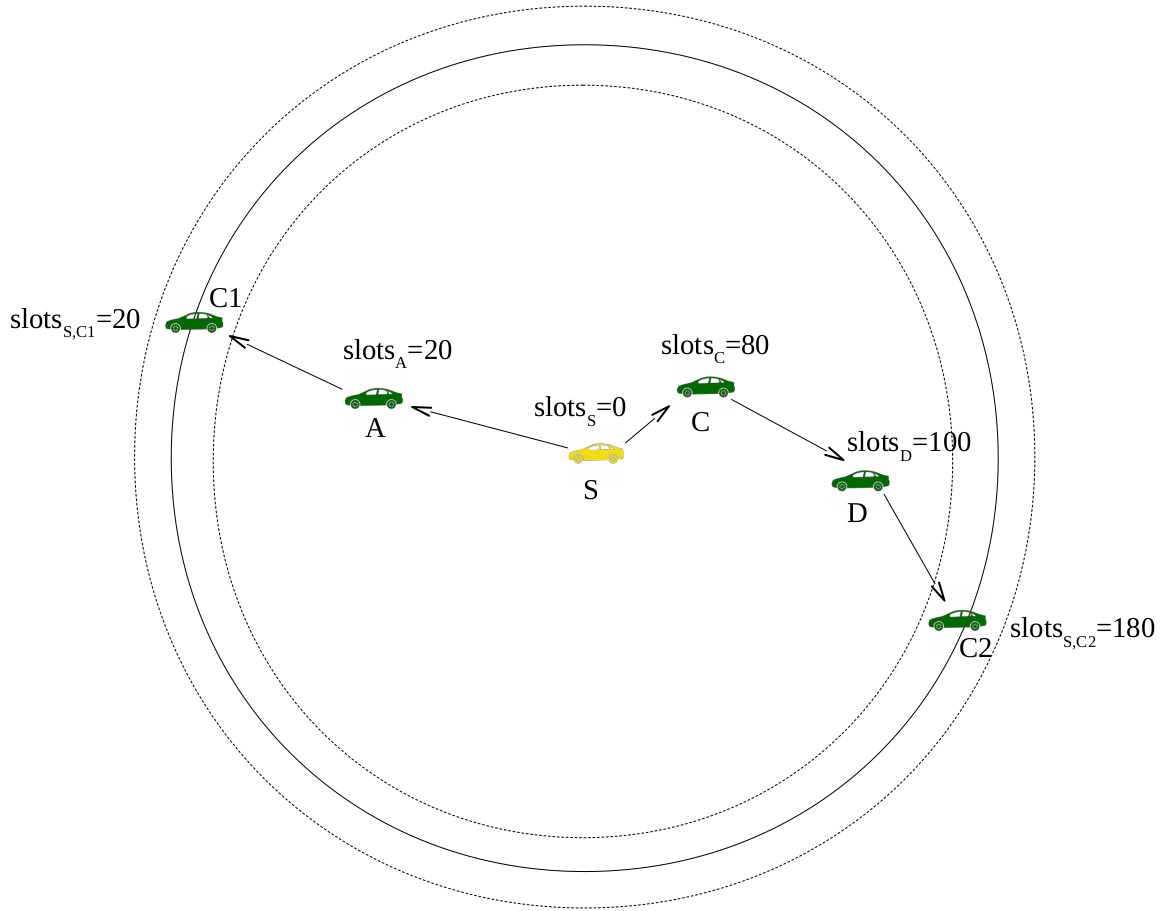
\includegraphics[width=0.7\textwidth]{immagini/slots}
				\caption{Example of \textit{NOS} calculation with Alert Message starting from node S}
				\label{fig:slots}
			\end{figure}
			
			
		\subsection{Forward Node Ratio (FNR)}
			This metric is used to measure the number of vehicles which forward the Alert Message. The value of this metric is an indicator of the effectiveness of the multi-hop protocol in successfully suppressing scheduled transmissions from PFCs after the FFC has relayed the message. The metric is calculated as follows:
			 
			\begin{gather}
				\label{eq:nos}
				NOH = \textrm{\textit{no. of vehicles forwarding the Alert Message}}
			\end{gather}	
				
	\section{Platoon scenario}
		The first scenario taken into consideration is a simple platoon scenario, where vehicles are placed in a strip-like area 15 kilometers long. Vehicles are 25 meters distant from each other.  Transmission ranges of 100, 300 and 500 has been employed during simulations. 
		Parameters for this scenario are included in Table \ref{table:platoon}.  
		
		\begin{table}[H]
			\def\arraystretch{1.1}
			\rowcolors{2}{D}{P}	
			\begin{tabularx}{\textwidth}{l | l  l}
				\rowcolor{I} {\large \textcolor{white}{Parameter}} & {\large \textcolor{white}{Value}} & {\large \textcolor{white}{}} \TBstrut  \\
				\toprule
				\endhead
	%			\midrule[1pt]
				\rowcolor{P} \multicolumn{3}{c}{Scenario configuration} \\
				\midrule[1pt]
				Road length 							& 15000 				& m		\\
				Distance between vehicles 				& 25					& m		\\
				Circumference							& 14000					& m		\\
				Number of vehicles						& 600					& 		\\
				Source of alert message position		& Left of platoon		&		\\
				\midrule[1pt]
				\rowcolor{P} \multicolumn{3}{c}{Network configuration} \\
				\midrule[1pt]
				Packet size								& 164					& byte	\\	
				Transmission standard					& 802.11b				&		\\
				Frequency								& 2.4					& GHz	\\
				Channel bandwidth						& 22					& MHz	\\
				Transmission speed						& 11					& Mbps	\\
				Transmission powers						& -7.0, 4.6, 13.4		& dBm	\\
				Transmission range						& 100, 300, 500			& m		\\
				Modulation								& DSSS					& 		\\
				Propagation loss model					& ns3::TwoRayGround 	&		\\
				Shadowing model							& None					&		\\
				Propagation delay model					& ns3::ConstantSpeed	&		\\
				\midrule[1pt]
				\rowcolor{P} \multicolumn{3}{c}{Protocols configuration} \\
				\midrule[1pt]
	%			Protocols tested						& \makecell{FB, ROFF, STATIC100, \\ STATIC300, STATIC500} & \\
				FB contention window					& [32, 1024]			& slot	\\
				ROFF distance range (\textit{k} parameter) & 1					&		\\	
				\midrule[1pt]
				Number of simulations per configuration	& 1000					&		\\
				\bottomrule
			\end{tabularx}
			\label{table:platoon}
			\caption{Platoon scenario configuration}
		\end{table}
	
		\begin{figure}[H]
			\centering
			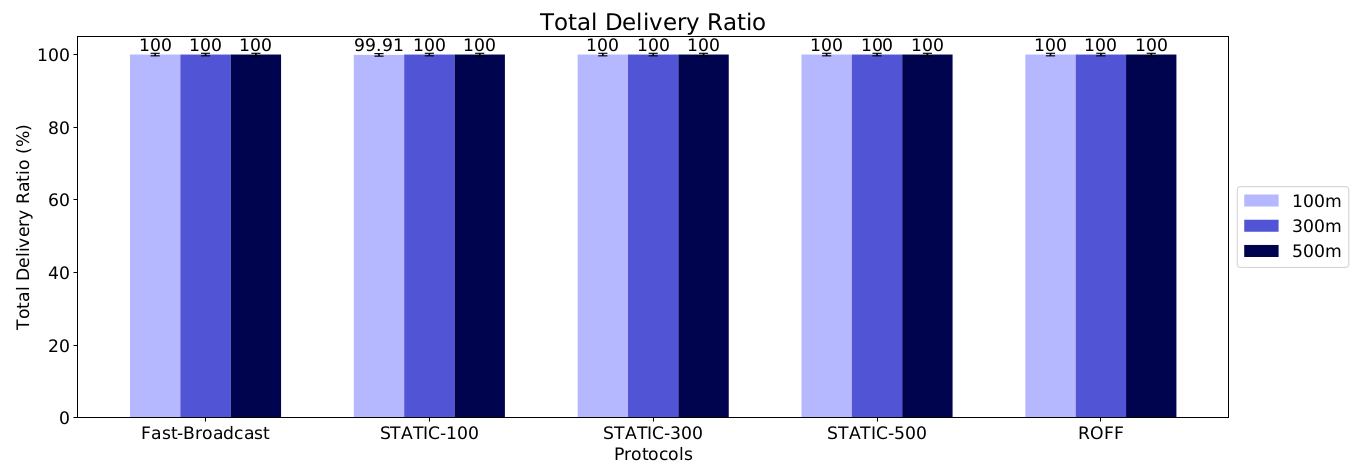
\includegraphics[width=1.1\textwidth]{immagini/platoon-15km/tdr}
			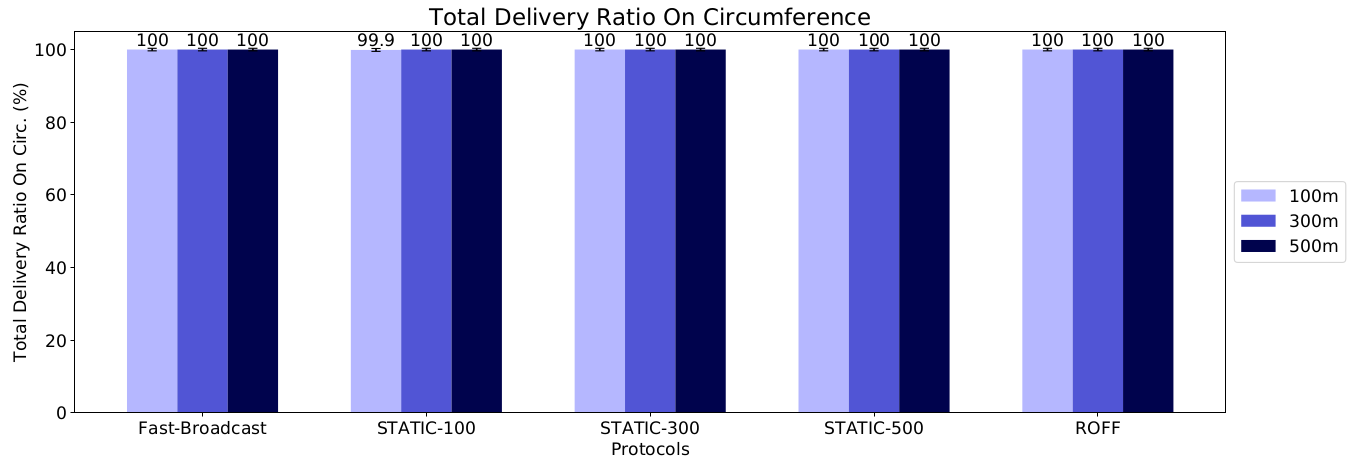
\includegraphics[width=1.1\textwidth]{immagini/platoon-15km/tdroc}
			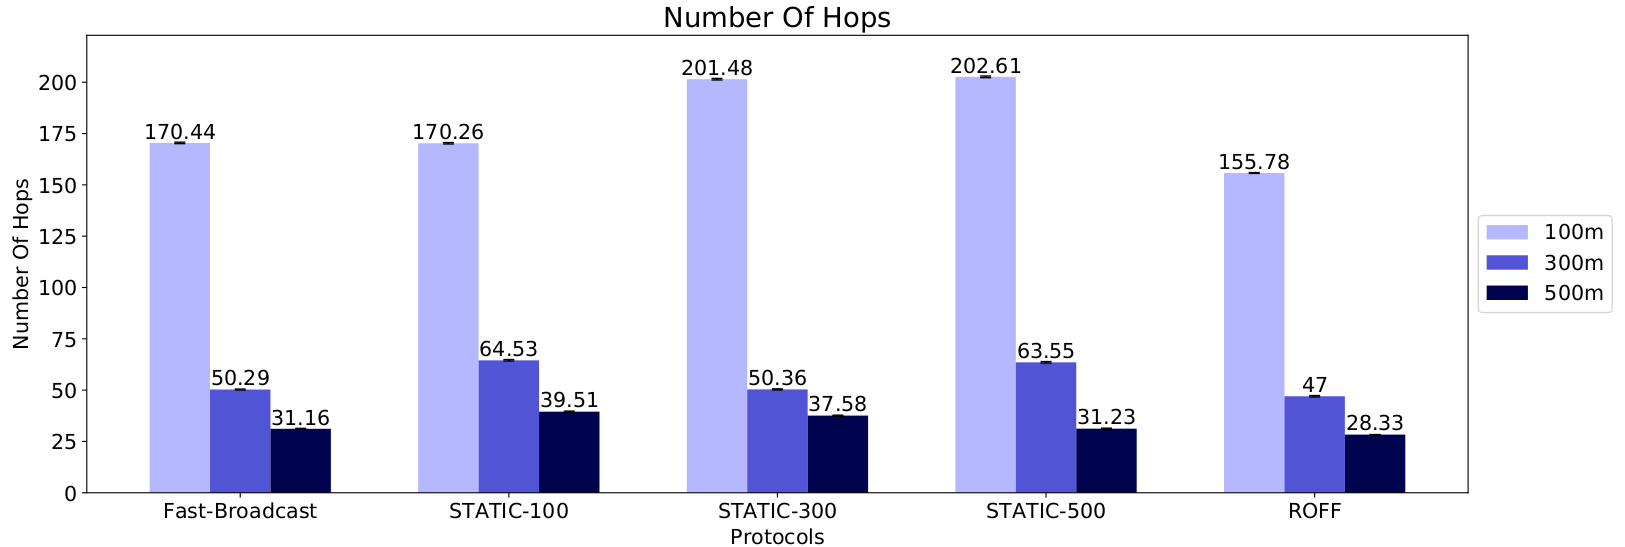
\includegraphics[width=1.1\textwidth]{immagini/platoon-15km/noh}
			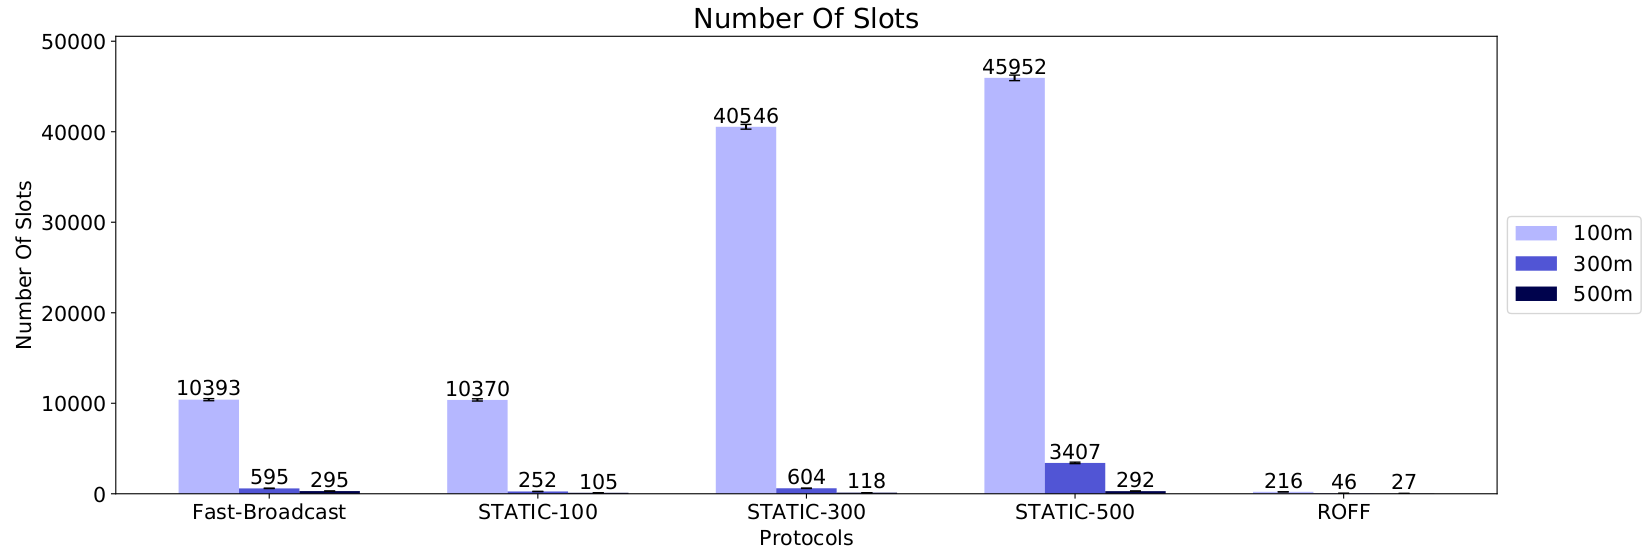
\includegraphics[width=1.1\textwidth]{immagini/platoon-15km/nos}
			\caption{\textit{TDR}, \textit{TDROC}, \textit{NOH} and \textit{NOS} metrics for Platoon scenario}
			\label{fig:metric-platoon-15km-1}
		\end{figure}

		\begin{figure}[H]
			\centering
			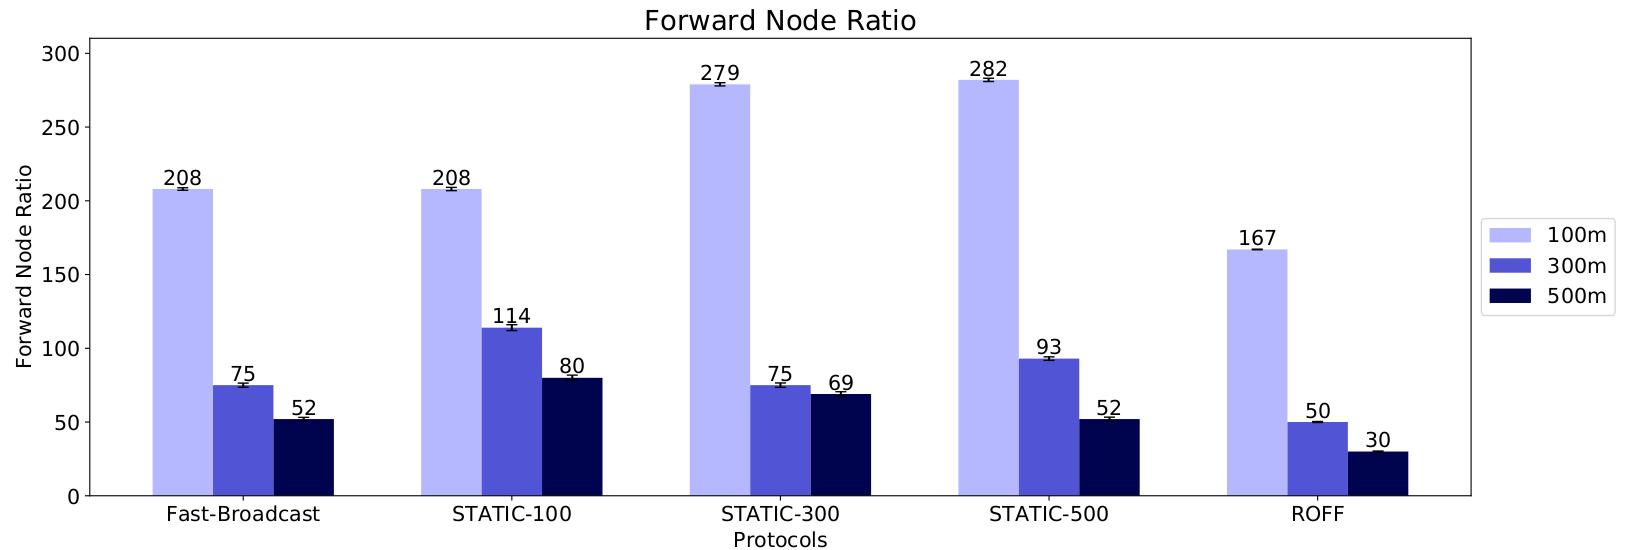
\includegraphics[width=1.1\textwidth]{immagini/platoon-15km/fnr}
			\caption{\textit{FNR} metric for Platoon scenario }
			\label{fig:metric-platoon-15km-2}
		\end{figure}
	
		Since this scenario is one-dimensional, the circumference simply consists in vehicles distant $14.000  \pm 12$ meters from the source of Alert Message. Both metrics about Delivery Ratio (global and on circumference) are close to 100\%, so the algorithms successfully propagate the AM until the end of the platoon.
		
		
		Considering the Number Of Hops, ROFF's results are 11,76\%, 6,54\% and 9,08\% lower than Fast-Broadcast's results respectively for 100, 300 and 500 meters transmission range. ROFF's results are close to the optimal number of hops, respectively 140, 46,6 and 28 for the same transmission ranges as above. This means that the forwarder selection algorithms based on ESD Bitmap works better in choosing the farthest vehicle from the previous forwarder compared to the contention window approach for 1D scenarios. Considering STATIC variants of Fast-Broadcast, it is possible to observe that the STATIC-tx variant produces comparable results with Fast-Broadcast with \textit{tx} transmission range (e.g. STATIC-100 value is comparable to Fast-Broadcast with 100 meters transmission range), as expected. The STATIC protocol performs worse (hence the Number of Hops increases) whenever the transmission range is underestimated (e.g. STATIC-100 with 300 meters transmission range, compared to Fast-Broadcast with the same transmission range) or overestimated (e.g. STATIC-500 with 100 meters transmission range, compared to Fast-Broadcast with the same transmission range). This behaviour is expected, as reported in \cite{BAR2017}.
		
		
		Regarding the Number of Slots, ROFF's performs much better than Fast-Broadcast. The metric's value is decreased respectively by 97,92\%, 92,27\% and 90,85\%  using ROFF. The waiting time calculation, based on unique forwarding priority instead of distance, guarantees a much lower wait compared to Fast-Broadcast contention window approach. As before, STATIC approaches produce results comparable with Fast-Broadcast when the transmission range estimation is correct. Instead, the Number of Slots greatly increases when the transmission range is underestimated and decreases when the transmission range is overestimated. In this last case, the decrease in NOS comes with an increase in Number Of Hops reported in the previous paragraph, so an overestimation of transmission range is not desirable.
		
		
		Lastly, it is possible to see that ROFF's achieves a better suppression of redundant transmissions, guaranteeing a decrease of 19,71\%, 33,33\% and 42,31\$ respectively for each one of the transmission ranges considered.
		
		
	\section{Grid scenario}
		After tests on the 1D Platoon scenario have been carried out, the next step consisted in testing the algorithm's performances in a 2D Grid scenario, employing also the shadowing model.
		Parameters for this scenario are included in Table \ref{table:platoon}.  
		
		\begin{table}[H]
			\def\arraystretch{1.1}
			\rowcolors{2}{D}{P}	
			\begin{tabularx}{\textwidth}{l | l  l}
				\rowcolor{I} {\large \textcolor{white}{Parameter}} & {\large \textcolor{white}{Value}} & {\large \textcolor{white}{}} \TBstrut  \\
				\toprule
				\endhead
				%			\midrule[1pt]
				\rowcolor{P} \multicolumn{3}{c}{Scenario configuration} \\
				\midrule[1pt]
				Road length 							& 15000 				& m		\\
				Distance between vehicles 				& 25					& m		\\
				Circumference							& 14000					& m		\\
				Number of vehicles						& 600					& 		\\
				Source of alert message position		& Left of platoon		&		\\
				\midrule[1pt]
				\rowcolor{P} \multicolumn{3}{c}{Network configuration} \\
				\midrule[1pt]
				Packet size								& 164					& byte	\\	
				Transmission standard					& 802.11b				&		\\
				Frequency								& 2.4					& GHz	\\
				Channel bandwidth						& 22					& MHz	\\
				Transmission speed						& 11					& Mbps	\\
				Transmission powers						& -7.0, 4.6, 13.4		& dBm	\\
				Transmission range						& 100, 300, 500			& m		\\
				Modulation								& DSSS					& 		\\
				Propagation loss model					& ns3::TwoRayGround 	&		\\
				Shadowing model							& None					&		\\
				Propagation delay model					& ns3::ConstantSpeed	&		\\
				\midrule[1pt]
				\rowcolor{P} \multicolumn{3}{c}{Protocols configuration} \\
				\midrule[1pt]
				%			Protocols tested						& \makecell{FB, ROFF, STATIC100, \\ STATIC300, STATIC500} & \\
				FB contention window					& [32, 1024]			& slot	\\
				ROFF distance range (\textit{k} parameter) & 1					&		\\	
				\midrule[1pt]
				Number of simulations per configuration	& 1000					&		\\
				\bottomrule
			\end{tabularx}
			\label{table:platoon}
			\caption{Platoon scenario configuration}
		\end{table}
		


%		../../scripts/graphs/out/Platoon-15km/b0/j0-cw[32-1024]/totCoverage
	         
%% !TEX encoding = UTF-8
% !TEX TS-program = pdflatex
% !TEX root = ../tesi.tex

%**************************************************************
\chapter{Analisi dei requisiti}
\label{cap:analisi-requisiti}
%**************************************************************

\intro{Breve introduzione al capitolo}\\

\section{Casi d'uso}

Per lo studio dei casi di utilizzo del prodotto sono stati creati dei diagrammi.
I diagrammi dei casi d'uso (in inglese \emph{Use Case Diagram}) sono diagrammi di tipo \gls{uml} dedicati alla descrizione delle funzioni o servizi offerti da un sistema, così come sono percepiti e utilizzati dagli attori che interagiscono col sistema stesso.
Essendo il progetto finalizzato alla creazione di un tool per l'automazione di un processo, le interazioni da parte dell'utilizzatore devono essere ovviamente ridotte allo stretto necessario. Per questo motivo i diagrammi d'uso risultano semplici e in numero ridotto.

\begin{figure}[!h] 
    \centering 
    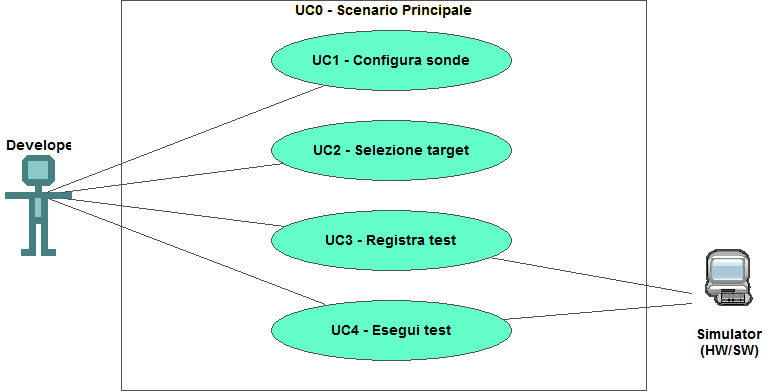
\includegraphics[width=0.9\columnwidth]{usecase/scenario-principale} 
    \caption{Use Case - UC0: Scenario principale}
\end{figure}

\begin{usecase}{0}{Scenario principale}
\usecaseactors{Sviluppatore applicativi}
\usecasepre{Lo sviluppatore è entrato nel plug-in di simulazione all'interno dell'IDE}
\usecasedesc{La finestra di simulazione mette a disposizione i comandi per configurare, registrare o eseguire un test}
\usecasepost{Il sistema è pronto per permettere una nuova interazione}
\label{uc:scenario-principale}
\end{usecase}

\section{Tracciamento dei requisiti}

Da un'attenta analisi dei requisiti e degli use case effettuata sul progetto è stata stilata la tabella che traccia i requisiti in rapporto agli use case.\\
Sono stati individuati diversi tipi di requisiti e si è quindi fatto utilizzo di un codice identificativo per distinguerli.\\
Il codice dei requisiti è così strutturato R(F/Q/V)(N/D/O) dove:
\begin{enumerate}
	\item[R =] requisito
    \item[F =] funzionale
    \item[Q =] qualitativo
    \item[V =] di vincolo
    \item[N =] obbligatorio (necessario)
    \item[D =] desiderabile
    \item[Z =] opzionale
\end{enumerate}
Nelle tabelle \ref{tab:requisiti-funzionali}, \ref{tab:requisiti-qualitativi} e \ref{tab:requisiti-vincolo} sono riassunti i requisiti e il loro tracciamento con gli use case delineati in fase di analisi.

\newpage

\begin{table}%
\caption{Tabella del tracciamento dei requisti funzionali}
\label{tab:requisiti-funzionali}
\begin{tabularx}{\textwidth}{lXl}
\hline\hline
\textbf{Requisito} & \textbf{Descrizione} & \textbf{Use Case}\\
\hline
RFN-1     & L'interfaccia permette di configurare il tipo di sonde del test & UC1 \\
\hline
\end{tabularx}
\end{table}%

\begin{table}%
\caption{Tabella del tracciamento dei requisiti qualitativi}
\label{tab:requisiti-qualitativi}
\begin{tabularx}{\textwidth}{lXl}
\hline\hline
\textbf{Requisito} & \textbf{Descrizione} & \textbf{Use Case}\\
\hline
RQD-1    & Le prestazioni del simulatore hardware deve garantire la giusta esecuzione dei test e non la generazione di falsi negativi & - \\
\hline
\end{tabularx}
\end{table}%

\begin{table}%
\caption{Tabella del tracciamento dei requisiti di vincolo}
\label{tab:requisiti-vincolo}
\begin{tabularx}{\textwidth}{lXl}
\hline\hline
\textbf{Requisito} & \textbf{Descrizione} & \textbf{Use Case}\\
\hline
RVO-1    & La libreria per l'esecuzione dei test automatici deve essere riutilizzabile & - \\
\hline
\end{tabularx}
\end{table}%           
%% !TEX encoding = UTF-8
% !TEX TS-program = pdflatex
% !TEX root = ../tesi.tex

%**************************************************************
\chapter{Analisi dei requisiti}
\label{cap:analisi-requisiti}
%**************************************************************

\intro{Breve introduzione al capitolo}\\

\section{Casi d'uso}

Per lo studio dei casi di utilizzo del prodotto sono stati creati dei diagrammi.
I diagrammi dei casi d'uso (in inglese \emph{Use Case Diagram}) sono diagrammi di tipo \gls{uml} dedicati alla descrizione delle funzioni o servizi offerti da un sistema, così come sono percepiti e utilizzati dagli attori che interagiscono col sistema stesso.
Essendo il progetto finalizzato alla creazione di un tool per l'automazione di un processo, le interazioni da parte dell'utilizzatore devono essere ovviamente ridotte allo stretto necessario. Per questo motivo i diagrammi d'uso risultano semplici e in numero ridotto.

\begin{figure}[!h] 
    \centering 
    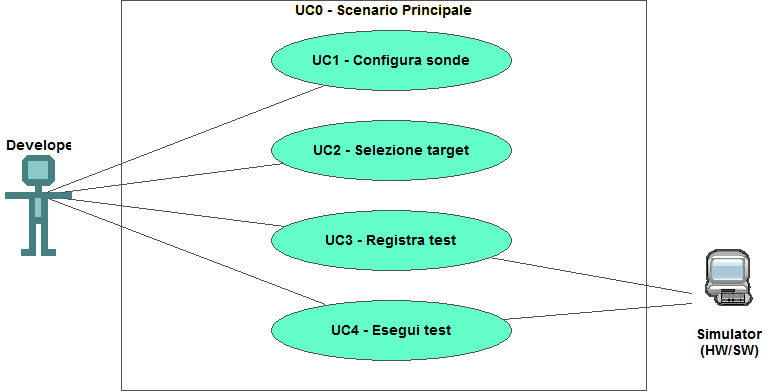
\includegraphics[width=0.9\columnwidth]{usecase/scenario-principale} 
    \caption{Use Case - UC0: Scenario principale}
\end{figure}

\begin{usecase}{0}{Scenario principale}
\usecaseactors{Sviluppatore applicativi}
\usecasepre{Lo sviluppatore è entrato nel plug-in di simulazione all'interno dell'IDE}
\usecasedesc{La finestra di simulazione mette a disposizione i comandi per configurare, registrare o eseguire un test}
\usecasepost{Il sistema è pronto per permettere una nuova interazione}
\label{uc:scenario-principale}
\end{usecase}

\section{Tracciamento dei requisiti}

Da un'attenta analisi dei requisiti e degli use case effettuata sul progetto è stata stilata la tabella che traccia i requisiti in rapporto agli use case.\\
Sono stati individuati diversi tipi di requisiti e si è quindi fatto utilizzo di un codice identificativo per distinguerli.\\
Il codice dei requisiti è così strutturato R(F/Q/V)(N/D/O) dove:
\begin{enumerate}
	\item[R =] requisito
    \item[F =] funzionale
    \item[Q =] qualitativo
    \item[V =] di vincolo
    \item[N =] obbligatorio (necessario)
    \item[D =] desiderabile
    \item[Z =] opzionale
\end{enumerate}
Nelle tabelle \ref{tab:requisiti-funzionali}, \ref{tab:requisiti-qualitativi} e \ref{tab:requisiti-vincolo} sono riassunti i requisiti e il loro tracciamento con gli use case delineati in fase di analisi.

\newpage

\begin{table}%
\caption{Tabella del tracciamento dei requisti funzionali}
\label{tab:requisiti-funzionali}
\begin{tabularx}{\textwidth}{lXl}
\hline\hline
\textbf{Requisito} & \textbf{Descrizione} & \textbf{Use Case}\\
\hline
RFN-1     & L'interfaccia permette di configurare il tipo di sonde del test & UC1 \\
\hline
\end{tabularx}
\end{table}%

\begin{table}%
\caption{Tabella del tracciamento dei requisiti qualitativi}
\label{tab:requisiti-qualitativi}
\begin{tabularx}{\textwidth}{lXl}
\hline\hline
\textbf{Requisito} & \textbf{Descrizione} & \textbf{Use Case}\\
\hline
RQD-1    & Le prestazioni del simulatore hardware deve garantire la giusta esecuzione dei test e non la generazione di falsi negativi & - \\
\hline
\end{tabularx}
\end{table}%

\begin{table}%
\caption{Tabella del tracciamento dei requisiti di vincolo}
\label{tab:requisiti-vincolo}
\begin{tabularx}{\textwidth}{lXl}
\hline\hline
\textbf{Requisito} & \textbf{Descrizione} & \textbf{Use Case}\\
\hline
RVO-1    & La libreria per l'esecuzione dei test automatici deve essere riutilizzabile & - \\
\hline
\end{tabularx}
\end{table}%             % Concept Preview
%% !TEX encoding = UTF-8
% !TEX TS-program = pdflatex
% !TEX root = ../tesi.tex

%**************************************************************
\chapter{Progettazione e codifica}
\label{cap:progettazione-codifica}
%**************************************************************

\intro{Breve introduzione al capitolo}\\

%**************************************************************
\section{Tecnologie e strumenti}
\label{sec:tecnologie-strumenti}

Di seguito viene data una panoramica delle tecnologie e strumenti utilizzati.

\subsection*{Tecnologia 1}
Descrizione Tecnologia 1.

\subsection*{Tecnologia 2}
Descrizione Tecnologia 2

%**************************************************************
\section{Ciclo di vita del software}
\label{sec:ciclo-vita-software}

%**************************************************************
\section{Progettazione}
\label{sec:progettazione}

\subsubsection{Namespace 1} %**************************
Descrizione namespace 1.

\begin{namespacedesc}
    \classdesc{Classe 1}{Descrizione classe 1}
    \classdesc{Classe 2}{Descrizione classe 2}
\end{namespacedesc}


%**************************************************************
\section{Design Pattern utilizzati}

%**************************************************************
\section{Codifica}
             % Product Prototype
%% !TEX encoding = UTF-8
% !TEX TS-program = pdflatex
% !TEX root = ../tesi.tex

%**************************************************************
\chapter{Verifica e validazione}
\label{cap:verifica-validazione}
%**************************************************************             % Product Design Freeze e SOP
%% !TEX encoding = UTF-8
% !TEX TS-program = pdflatex
% !TEX root = ../tesi.tex

%**************************************************************
\chapter{Conclusioni}
\label{cap:conclusioni}
%**************************************************************

%**************************************************************
\section{Consuntivo finale}

%**************************************************************
\section{Raggiungimento degli obiettivi}

%**************************************************************
\section{Conoscenze acquisite}

%**************************************************************
\section{Valutazione personale}
             % Conclusioni
%\appendix                               
%% !TEX encoding = UTF-8
% !TEX TS-program = pdflatex
% !TEX root = ../tesi.tex

%**************************************************************
\chapter{Appendice A}
%**************************************************************

\epigraph{Citazione}{Autore della citazione}



             % Appendice A

%**************************************************************
% Materiale finale
%**************************************************************
\backmatter
\printglossaries
% !TEX encoding = UTF-8
% !TEX TS-program = pdflatex
% !TEX root = ../tesi.tex

%**************************************************************
% Bibliografia
%**************************************************************

\cleardoublepage
\chapter{Bibliografia}

\nocite{*}
% Stampa i riferimenti bibliografici
\printbibliography[heading=subbibliography,title={Riferimenti bibliografici},type=book]

% Stampa i siti web consultati
\printbibliography[heading=subbibliography,title={Siti web consultati},type=online]


\end{document}